\title{Development of a Curved Layer Carbon Fiber 3D Printer}
\author{Jackie Song, Peter Ascoli}
\documentclass{article}
\usepackage[margin=1in]{geometry}
\usepackage[pdftex]{graphicx}
\usepackage{subcaption} %provides subfigure environment
\usepackage{epstopdf}
%\usepackage[autolinebreaks]{mcode}
\usepackage[section]{placeins}
\usepackage{gensymb}
\usepackage{mathtools}
\usepackage{siunitx}
\usepackage{fancyhdr}
\pagestyle{fancy}
\lhead{Peter Ascoli, Jackie Song}
\chead{Carbon Fiber 3D Printer}
\rhead{\rightmark}
\renewcommand{\headrulewidth}{0.4pt}
\renewcommand{\footrulewidth}{0.4pt}
\providecommand{\e}[1]{\ensuremath{\times 10^{#1}}}
\usepackage{setspace}
\usepackage{pdfpages}
\usepackage[hidelinks,colorlinks=false]{hyperref}
\usepackage[all]{hypcap}
\usepackage{grffile}
\usepackage{tablefootnote}

%REPORT REQUIREMENTS:
%
%1) Applies exceptional analytical skills and synthesis of knowledge at system design level
%2) Integrates concepts from different disciplines and recognizes applicability of concepts to design problem
%3) Clearly articulates design criteria and constraints
%4) Factors all constituents that contribute to design criteria and constraints and recognizes how design decisions impact design criteria and constraints
%5) Formulates clear problem statement
%6) Articulates problem solving process and outlines compelling strategy for finding quality solution
%7) Concise, well-organized and well-written
%8) Professional quality technical content
%9) Performs relevant and reputable literature review and demonstrates awareness of state-of-the-art

\begin{document}

%\maketitle

%---------------------------------------------------------
\begin{titlepage}
\center 

\hfill\\
\vspace{2cm}
\textsc{\LARGE ME164 Capstone Senior M/E Design} \\ 

\vspace{2.5cm} 

{\huge \textbf{DEVELOPMENT OF A CURVED LAYER \\[0pt] CARBON FIBER REINFORCED PLASTIC \\[10pt] 3D PRINTER}}\\[0.4cm] % Title of your document

\vspace{1.5cm} 
 
\large
\emph{by} \\
Jackie Song \\
Peter Ascoli

\vspace{1cm}

\large
\emph{Advised by} \\
Dr. Stan Wei 

\vspace{1.5cm} 

\textsc{\Large Deparment of Mechanical Engineering} \\
\textsc{\large The Cooper Union} \\
{\large May 2015} \\
\vfill 

\end{titlepage}


% ----------------------------------------------------------------------
%   filename:      abstract.tex
%   version:       1.1, 5/28/1997
%   description:   This is a LaTeX version 2.09 template 
%                  for the extended abstract of an ASME DETC paper.
%   usage:         latex abstract
% ----------------------------------------------------------------------
\documentstyle[11pt]{article}
\pagestyle{empty}

\setlength{\oddsidemargin}{1in}
\setlength{\evensidemargin}{1in}
\setlength{\marginparwidth}{0.0in}
\setlength{\topmargin}{0.5in}
\setlength{\headheight}{0in}
\setlength{\headsep}{0in}
\setlength{\textwidth}{4.5in}
\setlength{\textheight}{7.5in}
\setlength{\parindent}{0.25in}
\setlength{\parskip}{0.0in}

%%%% Change detc to the short name of your conference %%%%%%%%%%%%%
\def\confshortname{detc}
%%%% Change 1998 to the year of the conference %%%%%%%%%%%%%%%%%%%%
\def\confyear{1998}

\begin{document}

\newfont{\hvb}{cmssbx10}
\newfont{\hv}{cmss10}
\newfont{\tir}{cmr10}

\setlength{\baselineskip}{10pt}
{\scriptsize{\hvb
\begin{flushright}
%Extended Abstract \\
%%%%%%%%%%%%%%%%%%%%%%%  paper number %%%%%%%%%%%%%%%%%%%%%%%%%%%
DETC98/DAC-1234      %% change DETC98/DAC-1234 to the paper number
                     %% provided by ASME for your paper.
\end{flushright}
}}

\begin{center}
{\footnotesize{\hvb
%%%%%%%%%%%%%%%%%%%%%%%%%  paper title   %%%%%%%%%%%%%%%%%%%%%%%%%%%%%%%%%%
AN ARTICLE CREATED USING \LaTeX\ IN ASME FORMAT\\
}}

\vspace{10pt}
\setlength{\baselineskip}{11pt}

%%%%%%%%%%%%%%%%%%%%%%%%%   first author %%%%%%%%%%%%%%%%%%%%%%%%%%%%%
{\footnotesize
{\hvb Harry H. Cheng}, {\hv Associate Professor} \\
{\hv
Integration Engineering Laboratory\\
Department of Mechanical and Aeronautical Engineering \\
University of California, Davis, CA 95616\\
Tel: 530-752-5020, Fax: 530-752-4158\\ 
Email: hhcheng@ucdavis.edu, WWW: http://iel.ucdavis.edu\\
}}

\vspace{10pt}
%%%%%%%%%%%%%%%%%%%%%%%%%   Second/Third authors %%%%%%%%%%%%%%%%%%%%%%%%%%%%%
{\footnotesize
{\hvb First Coauthor}, {\hv Title} \\
{\hvb Second Coauthor}, {\hv Title} \\
{\hv
Department or Division Name \\
Company or College Name\\
City, State, Zip Code, Country (only if not U.S.)\\
Phone number, Fax number \\ 
Email address, WWW URL address\
}}

%%%%%%%%%%%%%%%% You may omit information for other authors %%%%%%%%%%%%%%%%%
%{\footnotesize
%{\hvb First Coauthor}, {\hv Title} \\
%{\hv
%Department or Division Name \\
%Company or College Name\\
%}}

\end{center}

\vspace{22pt}
%%%%%%%%%%%%%%%%%%%%%%%%%    Abstract Text    %%%%%%%%%%%%%%%%%%%%%%%%%%%%%
{\footnotesize{\tir
This article illustrates preparation of the extended abstract of
an ASME paper using \LaTeX.
The \LaTeX\  template \verb+abstract.tex+
that creates this extended abstract is available on the WWW at
the conference Web site 
or at \verb@http://iel.ucdavis.edu/code/.@
The extended abstract of an ASME paper should not exceed one page
with keywords at the end.\\

Instructions for submitting the electronic version of 
an ASME paper through ftp for publication in the CD-ROM proceedings 
are given as follows:
\begin{itemize}
\item
Rename your files with paper number as file name (replace forword slash by underscore), 
plus a meaningful
suffix such as {\bf .ps} (Postscript), 
{\bf .tex} (\LaTeX),
{\bf .pdf} (Portable document format),
{\bf .WP} (WordPerfect),
{\bf .Word} (MS Word),
{\bf .doc} (Other word-processing format).
\item
Compress your files, {\bf Zip} for PC, {\bf Stuffit} for Mac, {\bf tar.Z} for Unix.
\item
Log in to {\bf ftp.edoc.com} as an 'anonymous' user.
\item
Use your email address as password.
\item
At the {\tt ftp} prompt, type {\tt cd \confshortname} to change to directory {\tt \confshortname}.
\item
Transfer files by {\tt put} command as follows,
\begin{verbatim}
 put DECT98_DAC_1234.tar.Z   (submit one tar file only for Unix)
 put DECT98_DAC_1234_abs.tex
\end{verbatim}
\item
Finish file transfer by {\tt quit} command.
\end{itemize}


\vspace{10pt}
{\bf Keywords:} ASME, paper format, \LaTeX.


%%%%%%%%%%%%%%%%%%%%%%%%%%%%%%%%%%%%%%%%%%%%%%%%%%%%%%%%%%%%%%
}}

\vspace{\fill}
{\scriptsize{\hv
\begin{flushbottom}
\begin{flushright}
Copyright \copyright\ \confyear\ by ASME
\end{flushright}
\end{flushbottom}
}}

\end{document}



\tableofcontents
\thispagestyle{plain}
\clearpage
\listoffigures
\listoftables

%----------------------------------------------------------
\section*{Nomenclature}

\begin{tabbing}

  XXXXXX \= \kill% this line sets tab stop

  $ABS$ \> Acrylonitrile Butadiene Styrene\\
  $PLA$ \> Polylactic Acid\\
  $FDM$ \> Fused Depostion Modeling\\
  $CFRP$ \> Carbon Fiber Reinforced Plastic, or Carbon Fiber Reinforced Polymer\\
  
\end{tabbing}

\clearpage
%----------------------------------------------------------
\section{Introduction}

\subsection{Problem Definition}

\indent

3D printing technologies offer the ability to produce new parts quickly, allowing faster and cheaper design iterations. However, commercially available Fused Deposition Modeling (FDM) 3D printers currently produce relatively weak parts due to the materials and print method used. They print using weak thermoplastics, most commonly polylactic acid (PLA) or acrylonitrile butadiene styrene (ABS), and deposit the material only in planar layers parallel to the build platform. Because of poor layer adhesion, this method yields parts that fail quickly under loading due to layers being sheared or pulled apart; this type of failure is particularly evident in parts with thin bosses or shells normal to the build plane, which offer very little surface area for layers to bond. Some parts may be rotated in the printer software to maximize layer contact area, but the planar layer limitation remains. These faults in FDM printers limit much of 3D printing to rapid prototyping applications (where strength is not necessary) despite high demand for printers that can produce stronger parts for use in load-bearing applications. Subsequently, there exists a need for 3D printers using alternative materials and layer formulations that are capable of printing stronger, more usable parts.\\

\subsection{Background Research}

\indent

Current research indicates curved layers as a promising alternative layer geometry and fiber reinforced polymers as stronger  materials for FDM printers. While many resources were used to develop the concept of this 3D printer, a few key sources demonstrated the feasibility and value of the idea.\\

Research into curved layer ABS FDM prints indicates that this layer configuration provides stronger adhesion and better conforms to contoured features. Close to 150\% strength increases were found in parts where critical stresses were located on contoured features. Furthermore, this research demonstrated the problems of using low resolution actuation systems in curved layer FDM, citing difficulty in precisely depositing the material when high-precision, industrial-grade nozzle translation systems are not used.\cite{cute-curves}\\

Research into the strength of carbon fiber cross-ply composites demonstrated dependence of part strength on the fiber angle (between a 0\degree - 90\degree pair and a 45\degree - 45\degree pair) between alternating flat layers. This research, out of the Oak Ridge National Laboratory, showed that tensile strength, shear strength, stiffness, and fatigue varied greatly depending on the cross-ply angles.\footnote{Note that cross-ply composites use long carbon fibers}\cite{ornl} Additional research has analyzed the effects of cross-ply angles \cite{cantilever} in flat FDM ABS parts. Once again, orientation angle played a significant role in the strength of the part. Surprisingly, experimental and theoretical results showed modal solutions (multiple fiber orientations yielding nearly identical peaks in mechanical properties).\\

Finally, one company, MarkForged\cite{markforged}, has come close to realizing the full capability of FDM with a proprietary continuous carbon fiber filament. This company has produced parts that are as strong but slightly less stiff than aluminum.\\

These crucial sources demonstrate the dependency of part strength on layer type and fiber orientation. They further show the promise of CFRPs, which indicates huge potential for combining CFRP filaments with a curved layer FDM method. With these two methods combined, strong parts made out of carbon fiber could be brought into the homes of general consumers, and industry could begin using 3D printed parts in load-bearing applications rather than for rapid prototyping.\\

\subsection{Project Approach}

\indent

To create stronger 3D printed parts we are developing a Curved Layer Carbon Fiber 3D Printer. The printer will utilize FDM techniques to deposit one continuous strand of a carbon fiber reinforced plastic (CFRP) filament in curved layers. This material will mirror existing, widely used fiber-reinforced polymer materials, such as carbon fiber and fiberglass composites. Using curved layers will orient fibers in optimal direction(s) for withstanding applied loads and provide more area for layer adhesion. Figure~\ref{fig:layers} shows how curved layers compare to the typical cartesian layer method. To achieve curved layers a serial robot arm with six degrees of freedom will be used instead of a typical cartesian coordinate robot. These extra degrees of freedom will allow the printer to lay material in any direction. In combination with precise control over toolpaths, the CFRP filament and curved layers will allow strong fibers to be oriented optimally for the desired mechanical properties of the part. These properties will be user-determined based on expected loading, surface finish, and other part requirements. Ultimately, experimental comparisons between curved layer FDM and standard FDM parts will quantify the increase ins strength and provide additional insights towards optimizing fiber orientation.\\

\begin{figure}[htp]
\centering
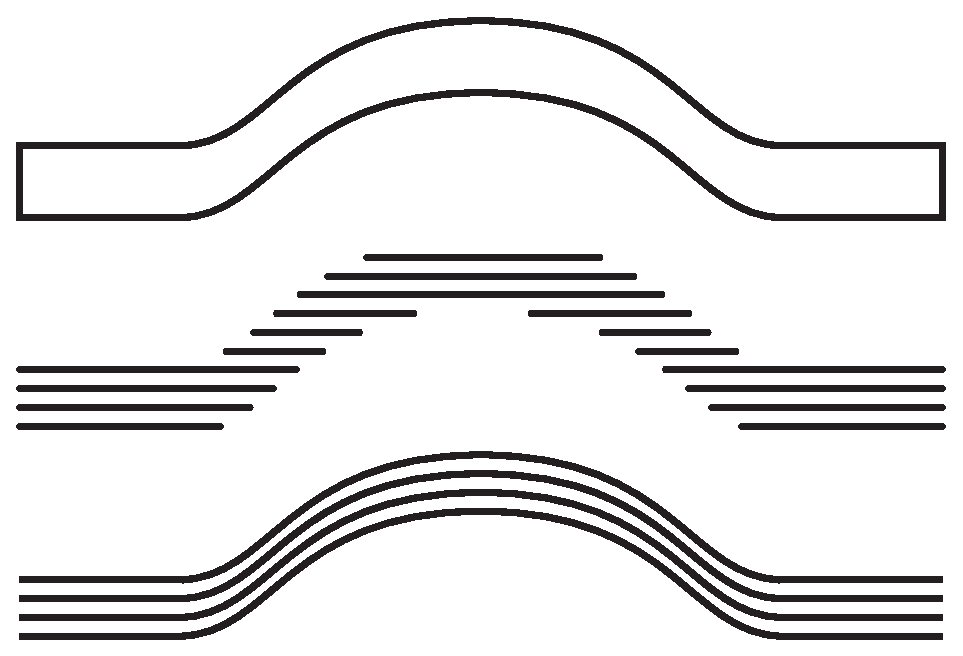
\includegraphics[width=0.5\textwidth]{./figures/layer-methods}
\caption{3D printing layer discretization methods. The desired part (top), typical planar/cartesian layers (middle), and curved layers (bottom).}
\label{fig:layers}
\end{figure}

To realize the goal of a fiber-reinforced composite curved layer 3D printer, the project was broken down into five subsystems, which are outlined in Figure~\ref{fig:flowchart}. First, all components of the 3D printing toolchain must be developed. The toolchain is defined by any hardware or software necessary for the steps between receiving a STereoLithography file (STL) and the printed part, which includes but is not limited to the extruder, control electronics, and the tool path generation scheme. Second, we must locate and learn to control a robot arm capable with six degrees of freedom. Third an appropriate CFRP with a usable ratio carbon fiber and thermoplastic matrix material is to be created. Fourth, computational and experimental methods can be utilized to determine optimal fiber orientation based on user requirements. Fifth, the printed parts will be experimental tests to quantify their mechanical properties. These five subsystems will come together to fully create the curved layer carbon fiber 3D printer.

\begin{figure}[htp]
\centering
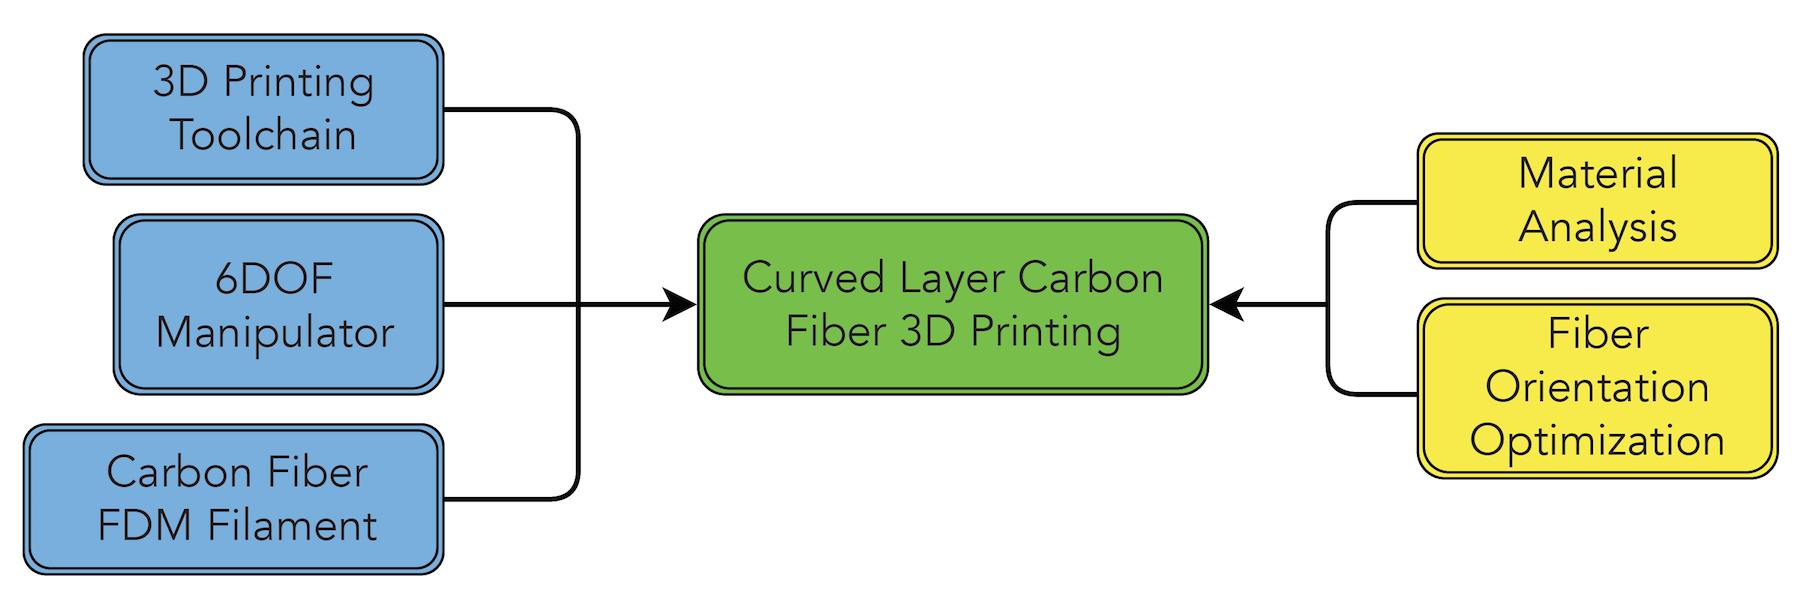
\includegraphics[width=0.75\textwidth]{./figures/flowchart}
\caption{A flow chart of subsystems.}
\label{fig:flowchart}
\end{figure}

%To realize the goal of a fiber-reinforced composite curved layer 3D printer, we will first learn to use to the FANUC LR Mate 200iC robot in The Cooper Union’s ME Rapid Prototyping Lab. This robot arm provides the necessary degrees of freedom for curved layer printing. We first plan to familiarize ourselves with the arm and control software by developing tool paths within its operational envelope. Then, we can mount an extruder to the arm and use an existing software toolchain to create standard flat-layer thermoplastic FDM prints. Once the standard print method is implemented, we can implement new gcode to create curved layer thermoplastic prints, while simultaneously investigating the best fiber composite to use as printing material. We will then alter the extruder mechanism to work with the chosen material. Finally, with curved layer fiber-reinforced 3D printing achieved, we plan to experimentally compare the mechanical strength of curved layer fiver-reinforced FDM prints to thermoplastic flat-layer FDM prints; the Instron machine in The Cooper Union’s ME Materials Lab can be used to load the parts and strain gauges can be attached to the parts to monitor specific local stresses.

%problem definition, background research, our project goal(s)
\clearpage

%----------------------------------------------------------
%\section{3D Printing Toolchain}

\subsection{Extruder}

\indent

The extruder is the mechanism responsible for depositing the filament in a 3D printing system. Generally, this mechanism includes a motor that drives a gripping mechanism, which reels in and pushes the filament into a heated nozzle. The nozzle heats the filament to a soft state and lays the filament on the printing bed or on an already printed layer to create the part.\\

In the case of the curved layer carbon fiber 3D printer, the extruder is required to mount to the robot arm, be compact\footnote{The compact size is required for two reasons. First, to ensure that induced torque on the robot arm joints and gripper remain within safe operating conditions. Second, to readily permit the nozzle to deposit material when not perpendicular to the build platform, which will be required for printing curved layers.}, and accept filaments of a variety of sizes (likely ranging in diameter from 1.75 mm to 3 mm). \\

Figure~\ref{fig:old extruder} presents the initial design of the extruder in \emph{SolidWorks}. The extruder mounts to the Fanuc grippers and is constructed out of a combination of machined aluminum parts and RepRap hardware (nozzle, J-head, J-head mounting plate, ceramic heating element, thermistor, fan, and fan mount). This configuration locates the nozzle outlet along the mid-plane of the grippers for simple coordinate transformations when programming the robot to print. Laser-cut acrylic gears provide a 3:1 step up in torque from the stepper motor and drive a notched screw, which grips and pushes the filament into the nozzle. A bearing opposite the screw provides counter-pressure and its mounting plates can adjust the distance between the screw and bearing to accommodate different filament sizes.\\

\begin{figure}[h!]
\centering
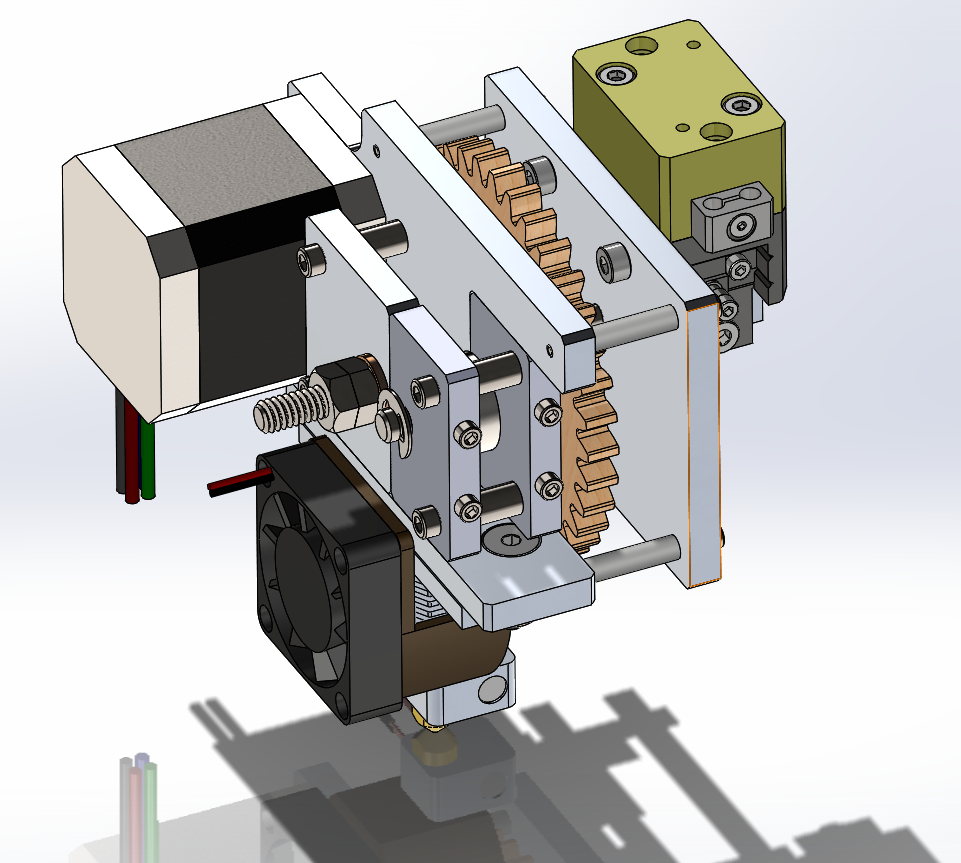
\includegraphics[width=0.5\textwidth]{./figures/extruder-old-2}
\caption{An isometric view of the initial extruder design.}
\label{fig:old extruder}
\end{figure}

To assess the feasibility of the initial extruder design, minor tweaks were implemented within the CAD to make a laser-cut prototype.  Figure~\ref{fig:prototype extruder} shows the prototype mounted on the FANUC grippers. The prototype served its purpose and demonstrated numerous problems with the initial design. There were some mis-measurements of RepRap hardware, using spacers instead of threaded standoffs decreased the rigidity of the structure, the structure was a bit larger than desired, and a few undetected interferences were discovered. Subsequently, the extruder then went through a series of redesigns to develop an acceptable configuration.\\

\begin{figure}[h!]
\centering
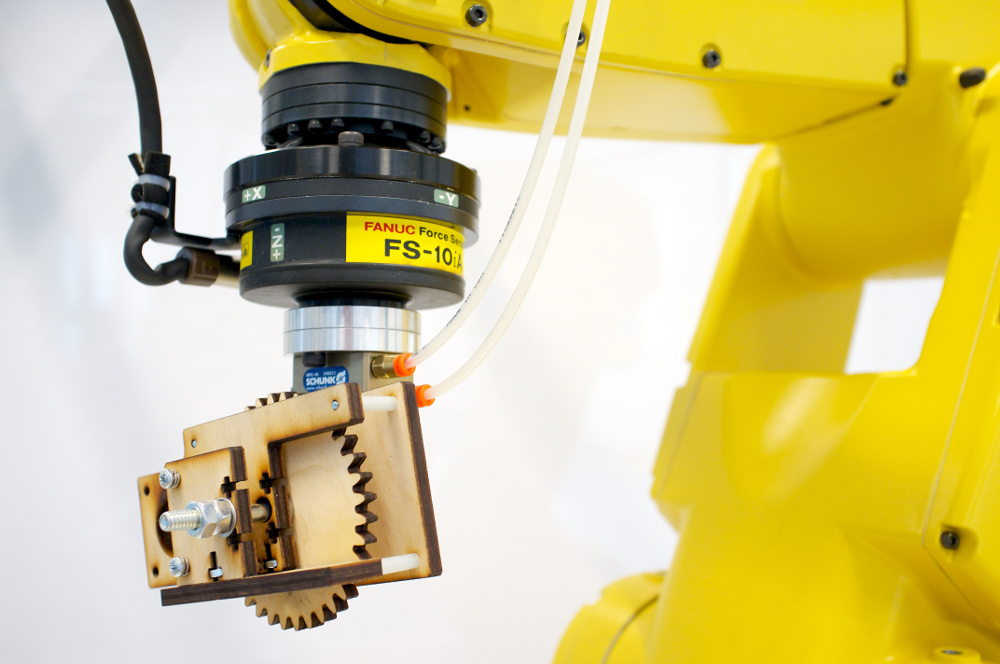
\includegraphics[width=0.5\textwidth]{./figures/extruder-prototype-2}
\caption{A photograph of the mounted prototype.}
\label{fig:prototype extruder}
\end{figure}

Figure~\ref{fig:extruder iso} presents a rendering of the final extruder design. Figure~\ref{fig:extruder drawing} provides general dimensions and annotations to fully present the extruder design concept. The final design is significantly smaller than the initial design, will require less machining, and uses less fastening hardware. The size decrease was accomplished by using smaller gears (50\% scaled versions of gears dimensions taken from \emph{SDP-SI}\footnote{\url{http://www.sdp-si.com/}} and located the stepper motor directly beneath the FANUC grippers. As part of the design process the gears were laser-cut, and physically tested to ensure that the teeth would not shear off under a load less than the stall torque of the stepper motor, before being fully committed to this design. The stepper motor (Sparkfun ROB-10846) outputs 68 oz-in of torque and has a resolution of 400 steps/revolution. Two laser-cut acrylic gears step up the torque to 204 oz-in.\footnote{Most extruders in the 3D printing community use analogous stepper motors and utilize gear trains to step up the torque. Common gear ratios range from 2:1 to 4:1 depending on the specific qualities of the filament. Given that the specifics of the filament are not yet fully determined, the mean value was used.} A partially threaded screw will be notched on the mill to contain teeth-like features along a portion of its length. These teeth will grip the filament and push it into the extruder. The screw rides along two bronze PTFE-coated bearings to ensure smooth rotation during printing. Two adjustment plates locate a bearing just opposite the screw to provide counter-pressure during printing. The plates are secured in place using four screws, which can be loosened or tightened to adjust the distance between the screw and bearing to accommodate different filament sizes. Shims or spring washers may have to be utilized to located this adjustable mechanism in its optimal position for the official CFRP.\\

The extruder will be machined with aluminum to provide rigidity. Many 3D printers utilize 3D printed bodies for mounting RepRap hardware, but the associated poor tolerances and material flexibility are not ideal for the curved layer carbon fiber 3D printer. Machining the extruder out of aluminum will allow easy implementation of any future adjustments and ensures all mechanisms will align properly. The entire extruder assembly secures to the FANUC gripper with four screws.\\

\begin{figure}[h!]
\centering
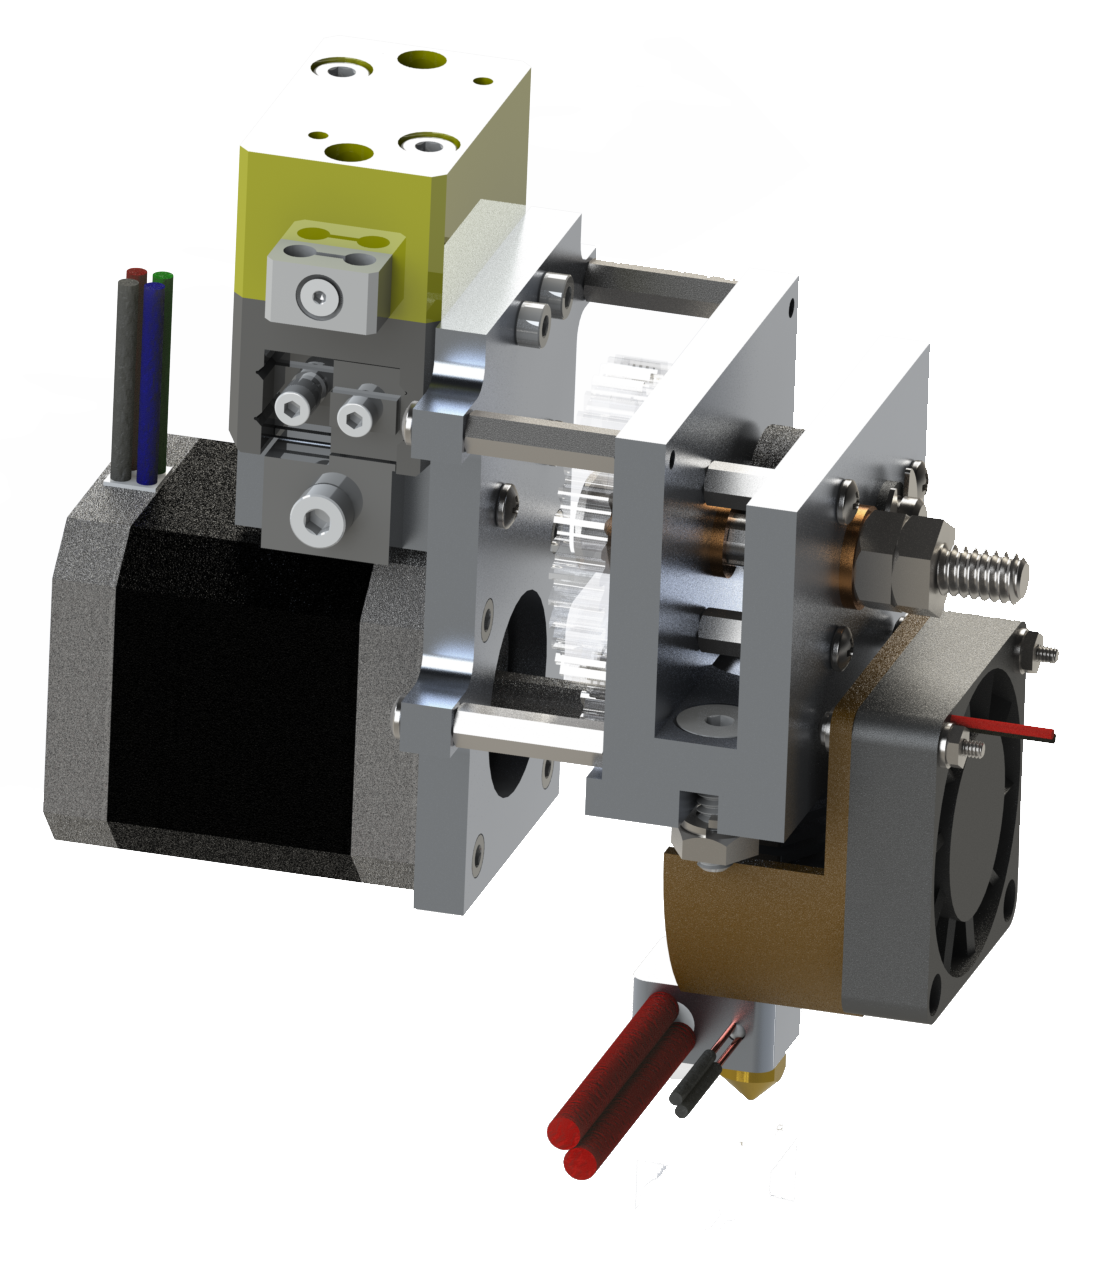
\includegraphics[width=0.5\textwidth]{./figures/extruder-iso}
\caption{An isometric render of the final extruder design.}
\label{fig:extruder iso}
\end{figure}

\begin{figure}[h!]
\centering
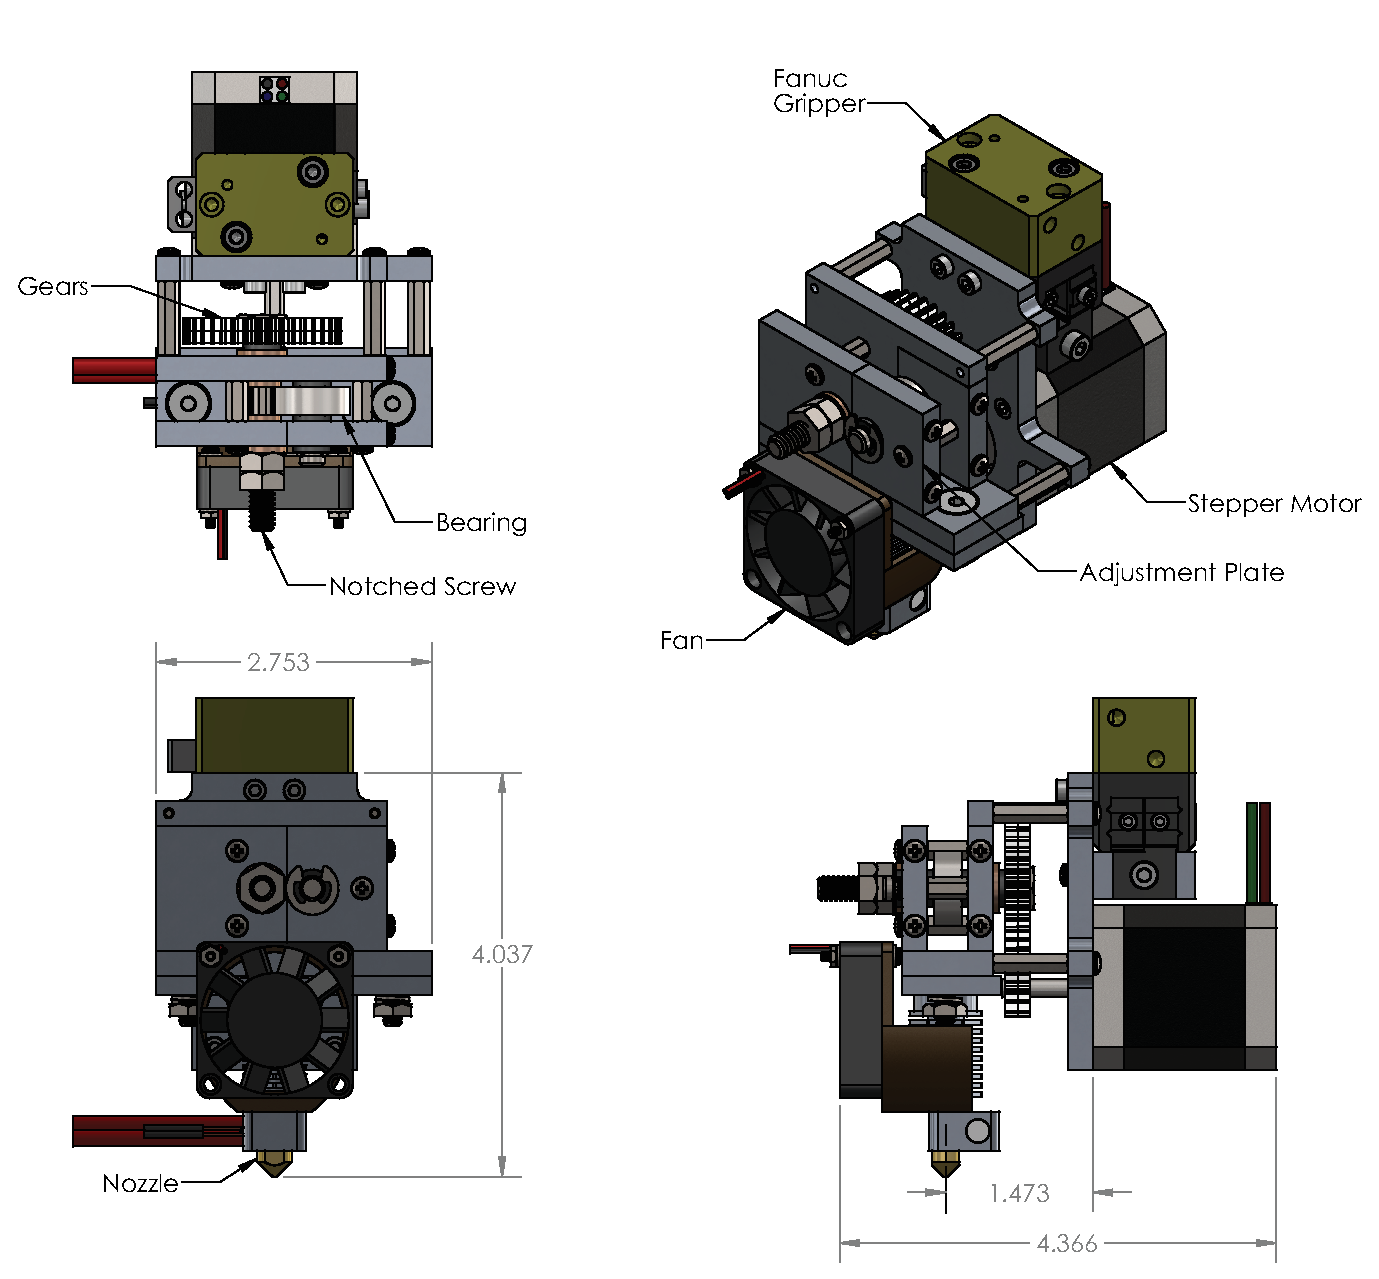
\includegraphics[width=1\textwidth]{./figures/extruder-drawing}
\caption{A general drawing of the final extruder design.}
\label{fig:extruder drawing}
\end{figure}

\clearpage




\subsection{Control Electronics}

\indent 

The extruder is controlled by a Megatronics control board, shown in Figure~\ref{fig:megatronics}, which was developed for the RepRap open source 3D printer project. The board contains all the necessary electronics to drive a Cartesian coordinate based FDM desktop 3D printer. The board can drive numerous positioning and extruder motors, heating elements, sensors, displays, and more. Because the FANUC robot handles the extruder positioning, the Megatronics board will be used to control the extruder elements only.\\

\begin{figure}[htp]
\centering
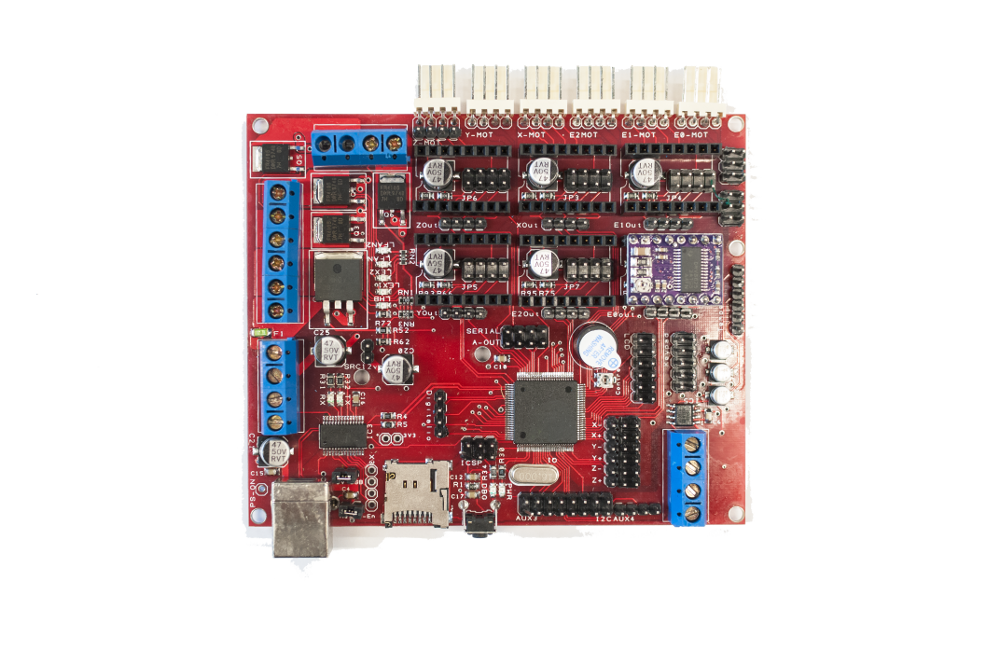
\includegraphics[width=0.5\textwidth]{./figures/electronics-board}
\caption{A photo of the Megatronics Control Board.}
\label{fig:megatronics}
\end{figure}

\subsubsection{Firmware}

\indent

When used in RepRap printers, the Megatronics board is typically used with one of several open source firmwares that are also associated with the RepRap project. Because these firmwares were designed with Cartesian desktop FDM printers in mind, they work well with the Megatronics board. The chosen firmware is uploaded to the board using a USB cable. For the FANUC-mounted extruder, a suitable firmware will be chosen and modified to work with the FANUC robot.\\

The firmware will be modified to control only the components present on the FANUC-mounted extruder. The firmware's timing functions must be modified as well. Normally, the firmware calculates its own filament feed rates and motor speeds in order to ensure that the flow rate of the extruded material follows the surface speed of the extruder with respect to the print surface. Because the FANUC controller has its own closed-loop control and is much less flexible than the RepRap firmware, the firmware will be modified to monitor the FANUC robot speed and position, and act accordingly. The monitoring will be accomplished by polling robot status system variables from a digital output on the FANUC controller.

\subsubsection{Enclosure}

\indent

The Megatronics board is too large to be mounted directly to the extruder, so it has been mounted inside the FANUC robot cage. The board is housed in a clear acrylic housing, shown in Figures~\ref{fig:megatronics-mount-back} and \ref{fig:megatronics-mount-front}, which serves several purposes. The housing protects the board from debris and accidental touches by either people or by the robot. The clear front makes the on-board status LEDs visible for debugging and operation. The back of the housing has built-in slots that provide anchors for cable management hardware. The cable management hardware will both organize the wires connected to the board and provide strain relief. The strain relief is especially important for the wires that connect the board and the extruder, because they will move with the extruder. The housing is positioned in a location that will cause the least interference between the wires and the arm. The power and USB cables for the board will be routed through the robot cage members. The USB cable will provide convenient access for updating the board firmware and collecting data using a laptop. 

\begin{figure}[htp]
\centering
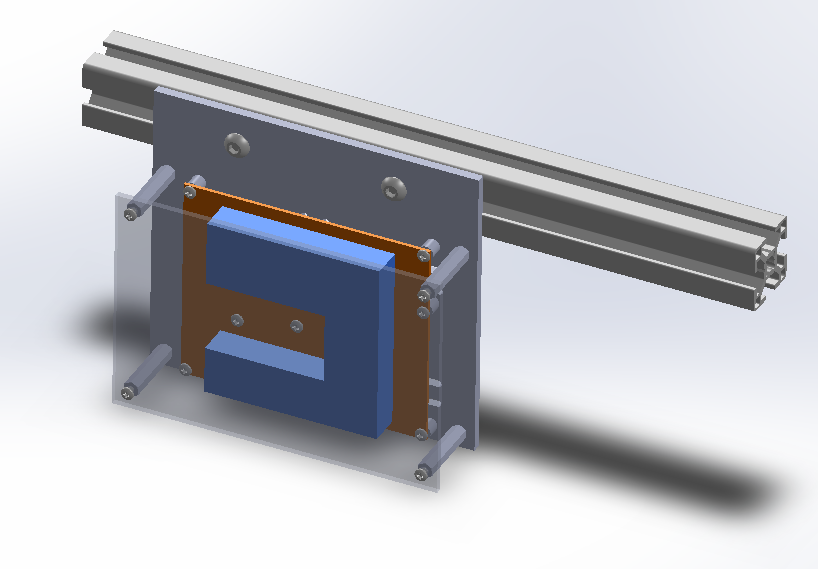
\includegraphics[width=0.5\textwidth]{./figures/megatronics-mount-1}
\caption{A \emph{SolidWorks} model of the mounted Megatronics board.}
\label{fig:megatronics-mount-back}
\end{figure}

\begin{figure}[htp]
\centering
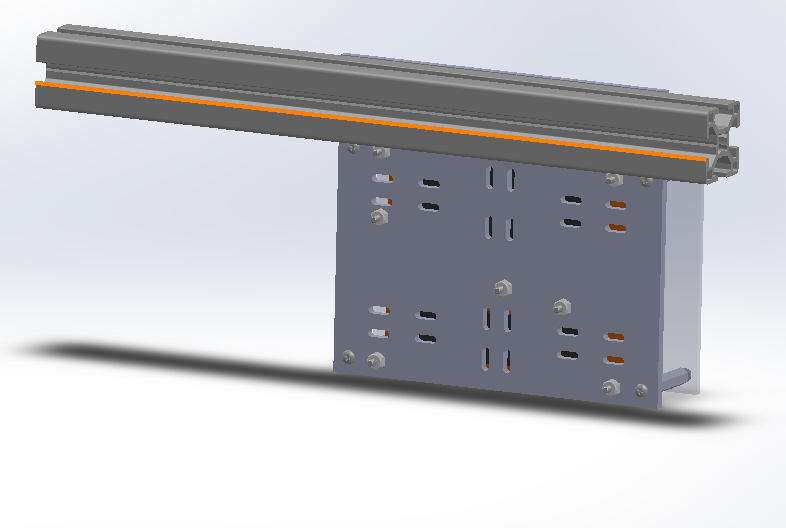
\includegraphics[width=0.5\textwidth]{./figures/megatronics-mount-2}
\caption{A \emph{SolidWorks} model of the mounted Megatronics board.}
\label{fig:megatronics-mount-front}
\end{figure}



%extruder, control electronics, slicing algorithm & layer generation
%\clearpage

%----------------------------------------------------------
%\section{6 Degree of Freedom Manipulator}

\indent

To extrude a consistent bead of material along a surface, the extruder nozzle should be normal to the surface. This means that in flat layer printing, the extruder may always be held vertically above the print surface. However, curved layers may require the extruder to tilt and rotate to reach some areas properly. Thus, curved layer FDM 3D printing requires the extruder positioning mechanism to have more degrees of freedom than flat-layer printing. \\

The FANUC LR Mate 200iC 6 degree of freedom industrial robot arm provides the necessary degrees of freedom for curved layer printing. The robot was acquired as part of an eductional package that includes the robot, its housing, the controller, a gripper and vision system, and related softwrae. The robot is compact and has positioning repeatable to 0.02 mm. As such, the robot is a suitable platform for a curved layer 3D printer. The extruder will be mounted to the existing gripper, and the control electronics and filament will be mounted to the side of the robot cage. Figure~\ref{fig:robot} provides a photograph of the FANUC robot itself, while Figure~\ref{fig:robot with things} shows a photograph of the FANUC with the electronics board and extruder.\\

%% talk about speed / position tracking and built in language?

\begin{figure}[htp]
\centering
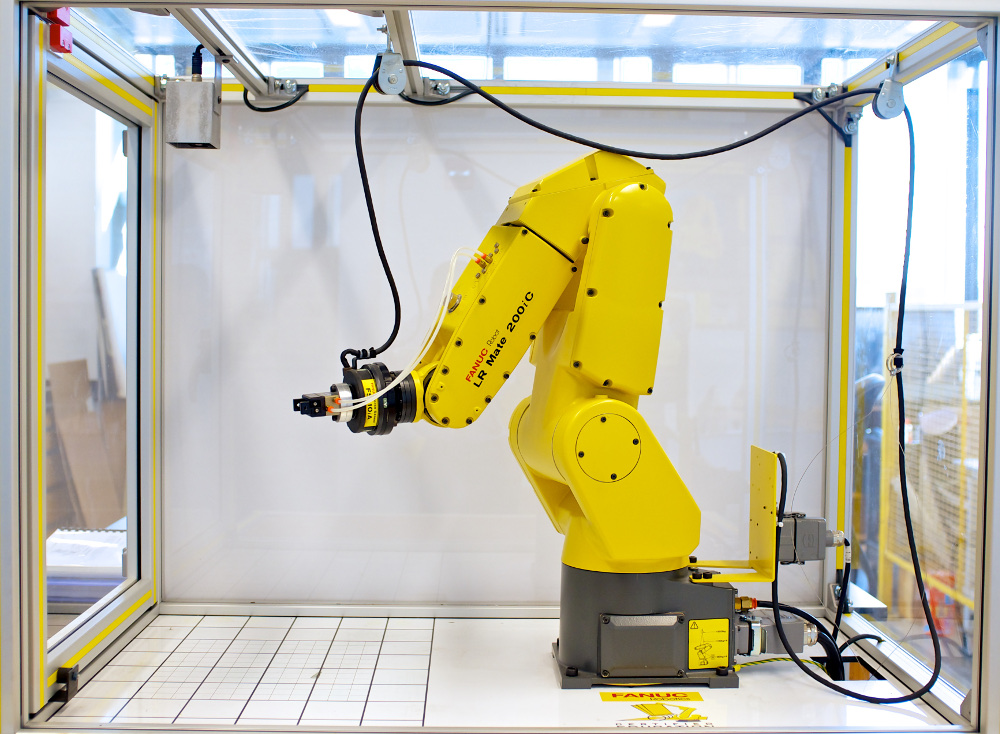
\includegraphics[width=0.5\textwidth]{./figures/robot}
\caption{A photograph of the FANUC LR Mate 200iC robot arm inside its cage.}
\label{fig:robot}
\end{figure}

\begin{figure}[htp]
\centering
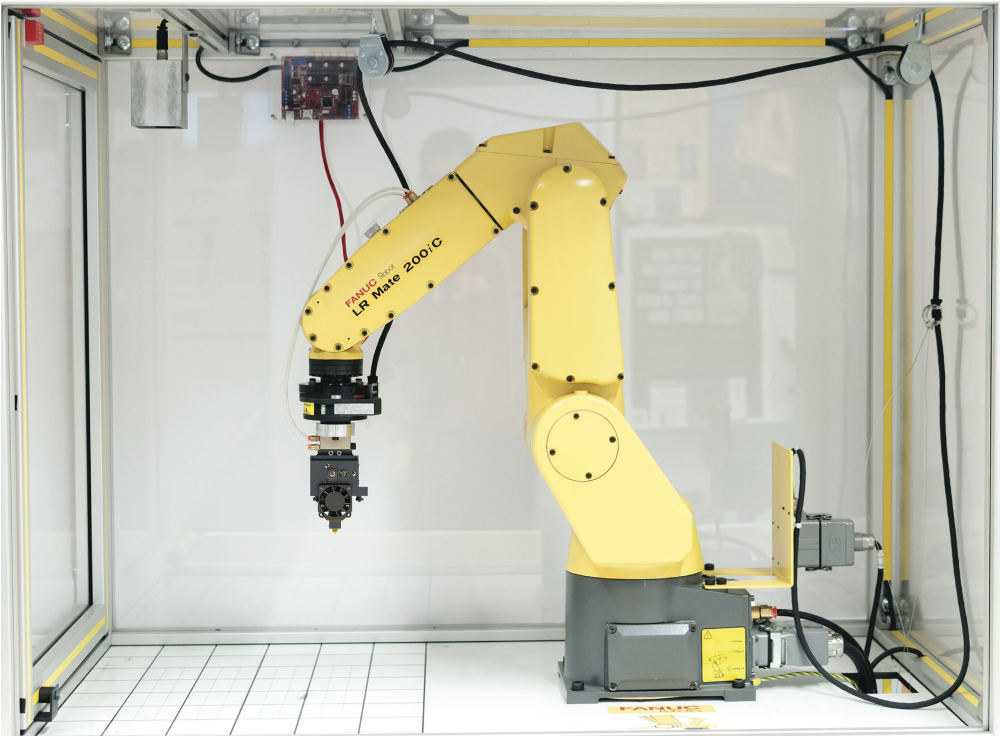
\includegraphics[width=0.5\textwidth]{./figures/robot-extruder-electronics}
\caption{A photograph of the robot with the mounted electronics and a rendering of the extruder.}
\label{fig:robot with things}
\end{figure}
%robots
%\clearpage

%----------------------------------------------------------
\section{Carbon Fiber Filament}

\indent

In order to print the CFRP material, carbon fiber and a resin were combined into a CFRP filament. As in conventional FDM printing, the CFRP filament is extruded by driving it through a heated nozzle. ABS plastic was chosen as the matrix material for this filament for several reasons. First, ABS has already successfully been combined with chopped carbon fiber in FDM filaments. Second, ABS does not require post-processing to reach full strength, as epoxy-based pre-impregnated carbon fiber composites do. In all filament development methods a 1K carbon fiber tow (shown in Figure~\ref{fig:carbon-fiber-spool}) was utilized.\\

\begin{figure}[htp]
    \centering
    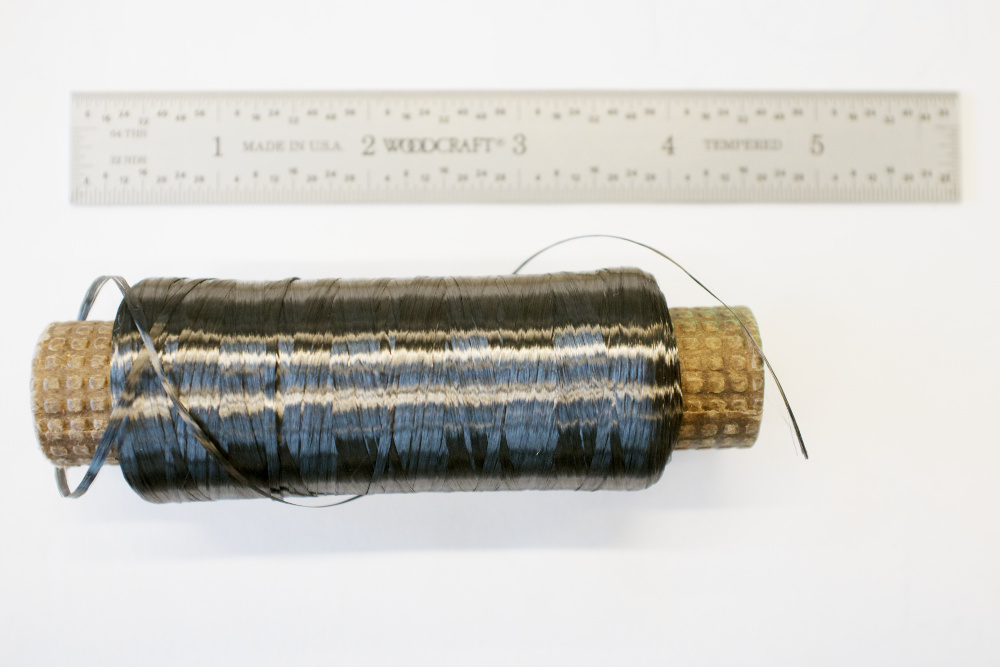
\includegraphics[width=0.5\textwidth]{./figures/carbon-fiber-spool}
    \caption{The 1K carbon fiber spool.}
    \label{fig:carbon-fiber-spool}
\end{figure}

\subsection{Production Methods}

\indent

Two proudction methods were explored for developing a CFRP filament. The first was pultrusion, an efficient fabrication method widely used to manufacture fiber-reinforced structural members. The second was a slurry dipping method, a tedious process where fibers were guided through a solution containing ABS, which would air dry onto the fibers and provide full fiber wet-out.\\

\subsubsection{Pultrusion}

\indent

A 3Doodler handheld 3D printing device was employed in pultrusion tests. The 3Doodler's feed motor was disabled, and then a bundle of carbon fiber and an ABS rod were simultaneously fed through the 3Doodler's heater and nozzle. The combined materials were manually drawn through from the exit end of the nozzle. This process is shown in Figure~\ref{fig:pultrusion-vid}. In the resulting filament, the carbon fiber bundle and the ABS adhered together well. However, due to the high viscosity of the heated ABS, most of the individual carbon fibers were not in contact with the ABS. Additionally, the fiber is not centered within the new CFRP filament, which is necessary printing.\footnote{Fibers located on the outside of the CFRP filament encounter a no-slip condition when entering the heated nozzle and subsequently never leave the nozzle with the ABS.} This effect is visible in Figure~\ref{fig:pultruded-scope}.\\

\begin{figure}[h!]
    \centering
    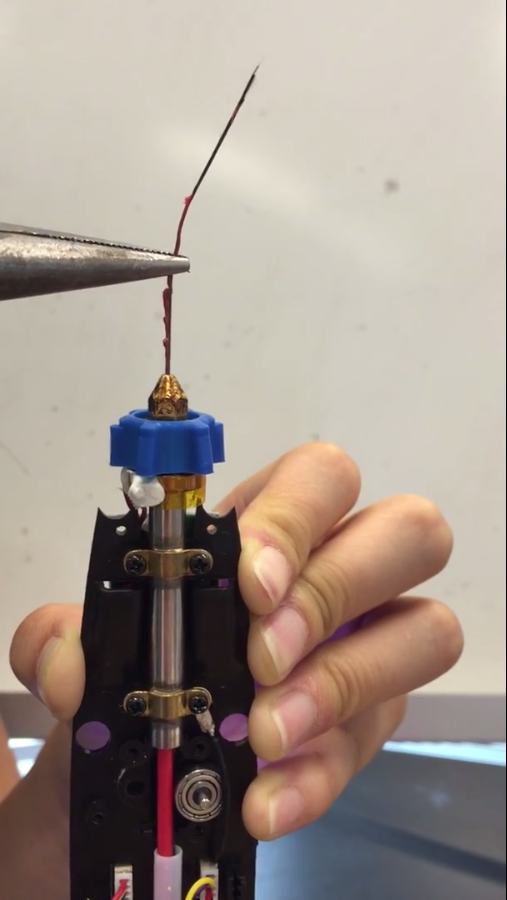
\includegraphics[width=0.4\textwidth]{./figures/pultrusion-vid}
    \caption{The experimental pultrusion setup, using the 3Doodler.}
    \label{fig:pultrusion-vid}
\end{figure}

\begin{figure}[h!]
    \centering
    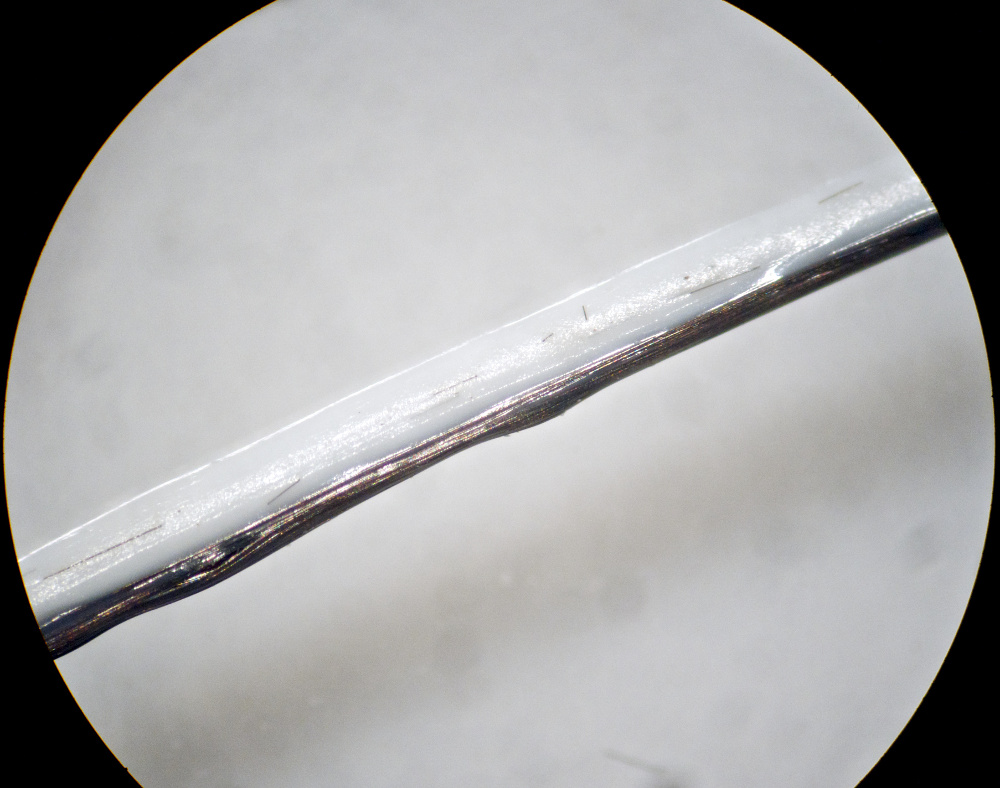
\includegraphics[width=0.6\textwidth]{./figures/pultruded-scope}
    \caption{Pultruded filament sample, magnified 10x under a microscope.}
    \label{fig:pultruded-scope}
\end{figure}

\clearpage

\subsubsection{Slurry Dipping}

Good fiber wet-out is critical to the performance of fiber composites, so another filament production method was explored. In the new procedure, achieving complete wet-out was prioritized. ABS plastic was dissolved in acetone to make a slurry. A fiber guide was fabricated to guide the carbon fiber in and out of the slurry. Carbon fiber bundles were then drawn through the fiber guide and allowed to dry. The process setup is shown in Figure~\ref{fig:dipping-vid}. As the acetone evaporated from the slurry, a small amount of ABS was left on the carbon fibers. The resulting filament showed very good wet-out. A pultruded sample and a dipped sample are shown side-by-side in Figure~\ref{fig:two-samples}.\\

\begin{figure}[h!]
    \centering
    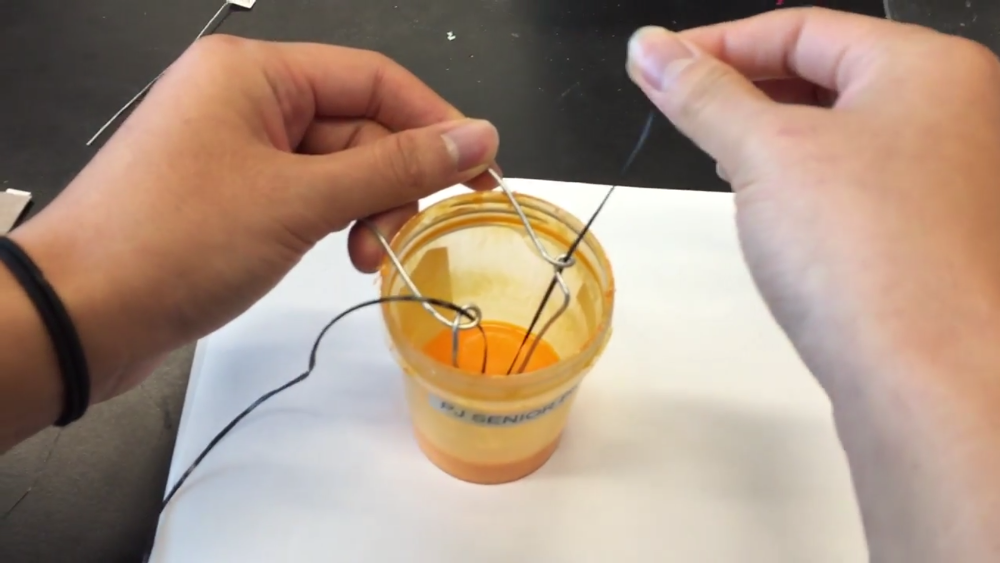
\includegraphics[width=0.8\textwidth]{./figures/dipping-vid}
    \caption{The basic slurry dipping process.}
    \label{fig:dipping-vid}
\end{figure}

\begin{figure}[h!]
    \centering
    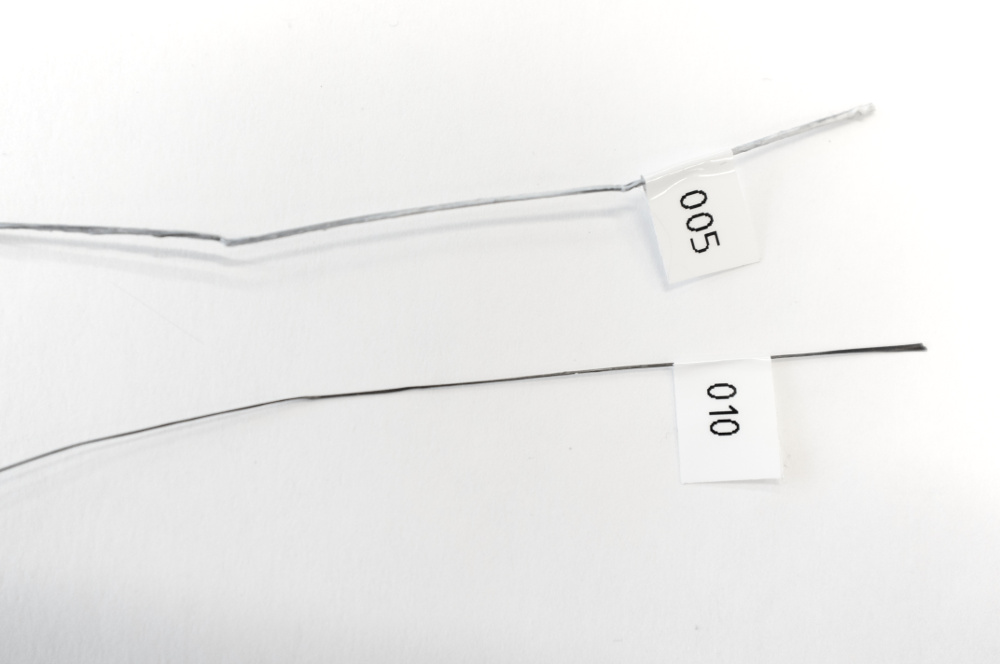
\includegraphics[width=0.6\textwidth]{./figures/FilamentSample}
    \caption{A pultruded filament sample (top) and a dipped filament sample (bottom), labeled with sample numbers.}
    \label{fig:two-samples}
\end{figure}

As the more promising of the two methods, dipping was explored further in attempt to create a viable CFRP filament.\\

%%% Slurry Photos



%%% Dipping Method Diagrams

%\begin{figure}[h!]
%    \centering
%    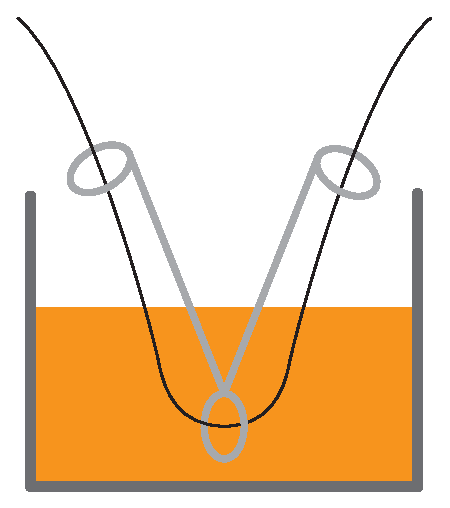
\includegraphics[width=0.5\textwidth]{./figures/external-dip-diagram}
%    \caption{An illustration of a wire-guided dipping method with the guide only partially immersed in the slurry.}
%    \label{fig:external-dip-diagram}
%\end{figure}
%
%\begin{figure}[h!]
%    \centering
%    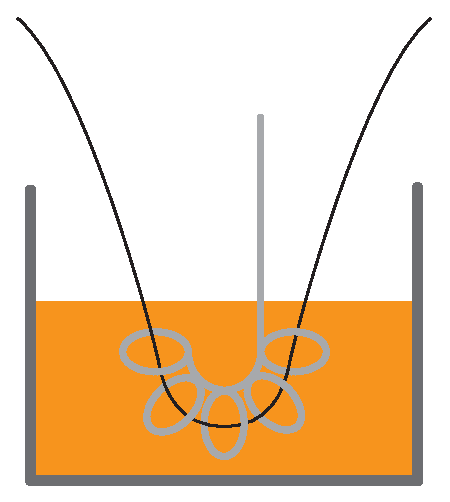
\includegraphics[width=0.5\textwidth]{./figures/internal-dip-diagram}
%    \caption{An illustration of a wire-guided dipping method with the guide fully immersed in the slurry.}
%    \label{fig:internal-dip-diagram}
%\end{figure}
%
%\begin{figure}[h!]
%    \centering
%    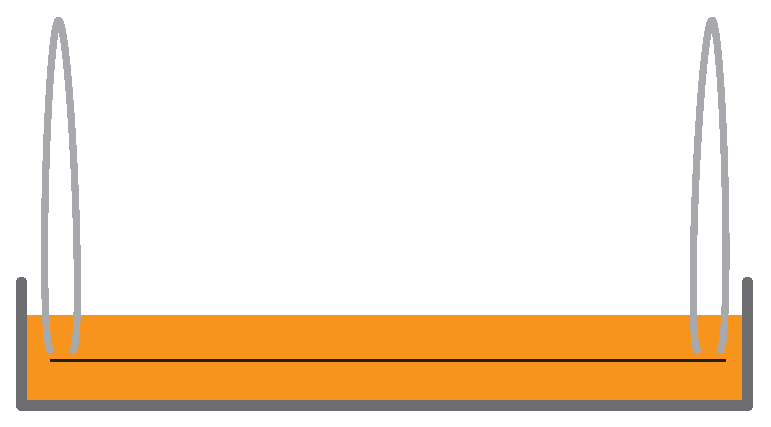
\includegraphics[width=0.5\textwidth]{./figures/flat-dip-diagram}
%    \caption{An illustration of the bath dipping method.}
%    \label{fig:flat-dip-diagram}
%\end{figure}

\begin{figure}[h!]
        \centering
        \begin{subfigure}[b]{0.3\textwidth}
                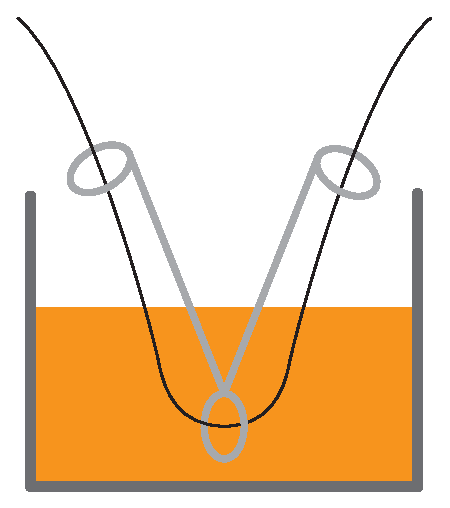
\includegraphics[width=\textwidth]{./figures/external-dip-diagram}
                \caption{Partially immersed guide.}
                \label{fig:external-dip-diagram}
        \end{subfigure}%
        ~ %add desired spacing between images, e. g. ~, \quad, \qquad, \hfill etc.
          %(or a blank line to force the subfigure onto a new line)
        \begin{subfigure}[b]{0.3\textwidth}
                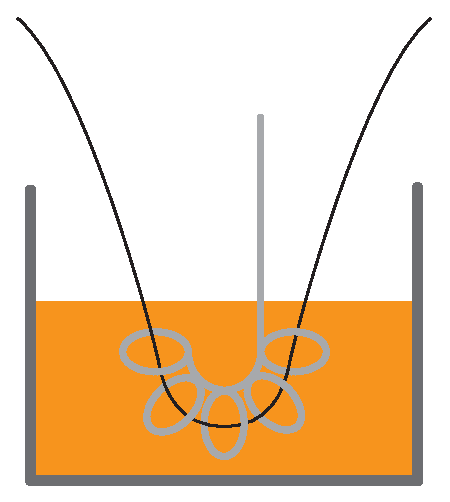
\includegraphics[width=\textwidth]{./figures/internal-dip-diagram}
                \caption{Fully immersed guide.}
                \label{fig:internal-dip-diagram}
        \end{subfigure}
        ~ %add desired spacing between images, e. g. ~, \quad, \qquad, \hfill etc.
          %(or a blank line to force the subfigure onto a new line)
        \begin{subfigure}[b]{0.3\textwidth}
                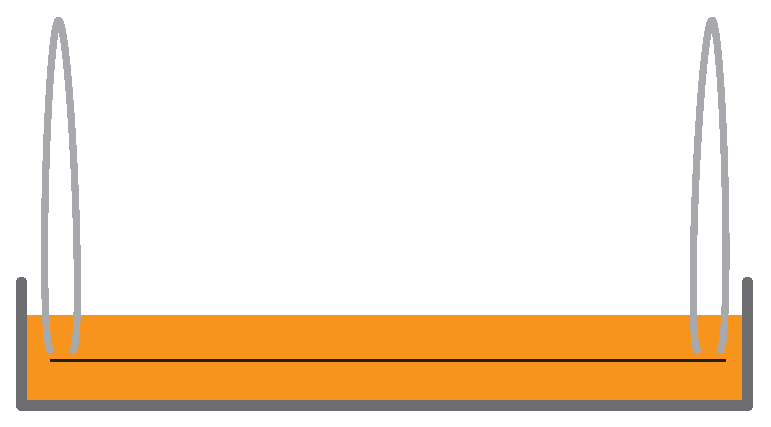
\includegraphics[width=\textwidth]{./figures/flat-dip-diagram}
                \caption{Bath dipping.}
                \label{fig:flat-dip-diagram}
        \end{subfigure}
        \caption{Slurry Dippng Methods.}\label{fig:dip-diagram}
\end{figure}

%%% slurry making photos

\begin{figure}[h!]
        \centering
        \begin{subfigure}[b]{0.3\textwidth}
                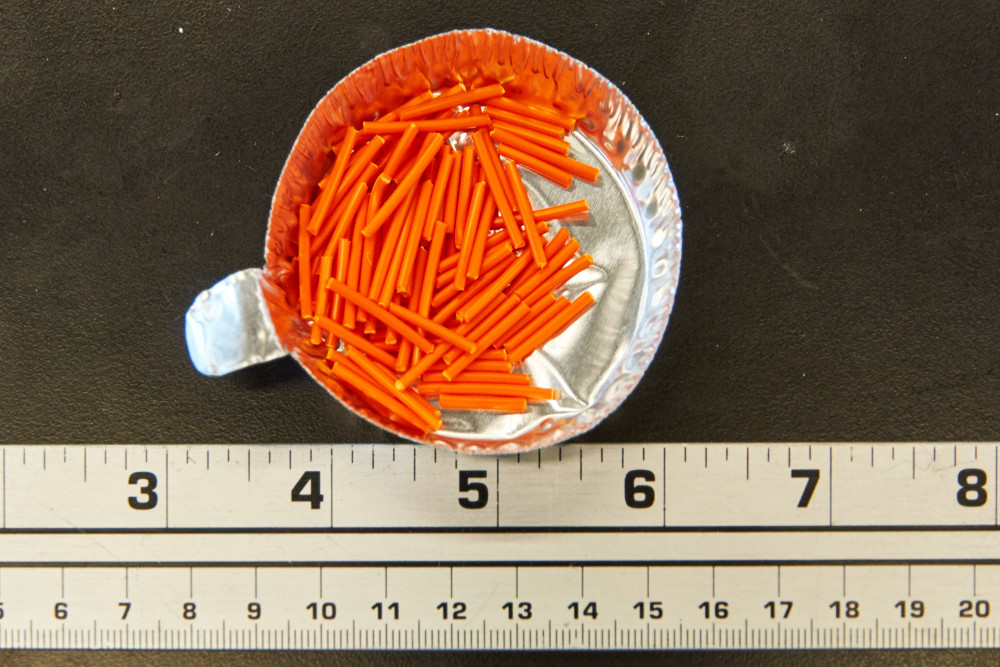
\includegraphics[width=\textwidth]{./figures/filament-abs-chopped}
                \caption{Chopped ABS.}
                \label{fig:filament-abs-chopped}
        \end{subfigure}%
        \begin{subfigure}[b]{0.3\textwidth}
                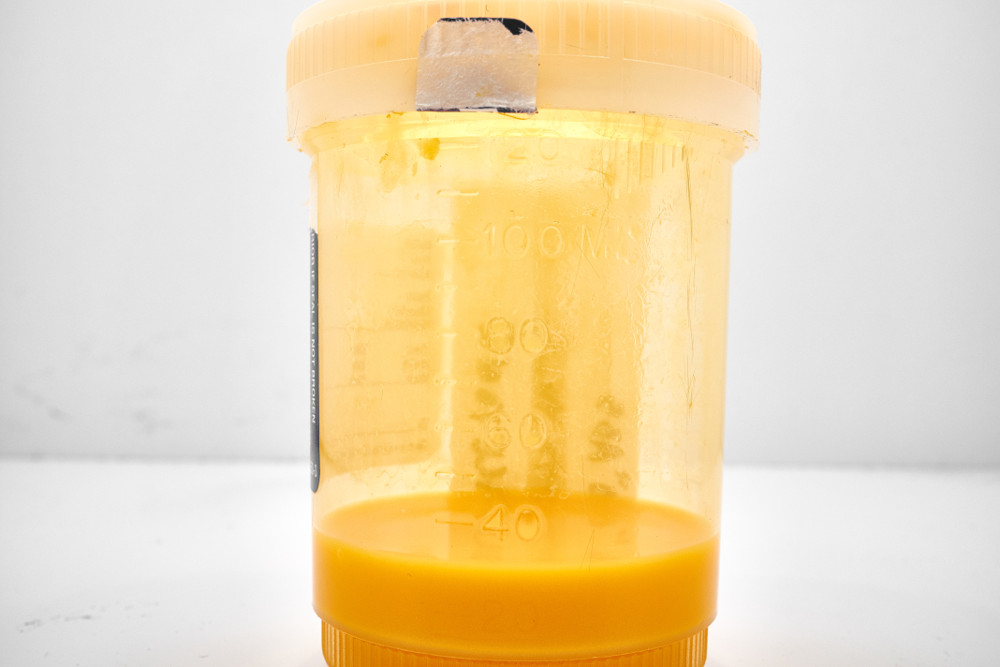
\includegraphics[width=\textwidth]{./figures/filament-mixture-volume-markings}
                \caption{Various mixtures.}
                \label{fig:filament-mixture-volume-markings}
        \end{subfigure}
        \begin{subfigure}[b]{0.3\textwidth}
                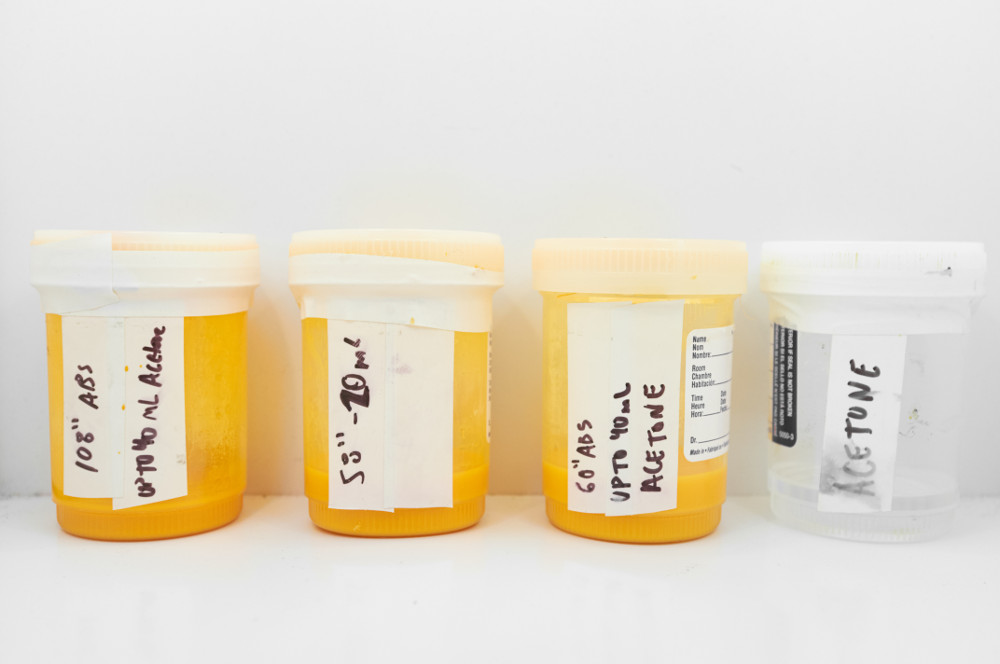
\includegraphics[width=\textwidth]{./figures/filament-mixtures}
                \caption{Volume markings.}
                \label{fig:filament-mixtures}
        \end{subfigure}
        \caption{Photos of the ABS-acetone slurry-making process}\label{fig:slurry-making}
\end{figure}

%%% Filament Photos

% external guide

\begin{figure}[h!]
        \centering
        \begin{subfigure}[b]{0.3\textwidth}
                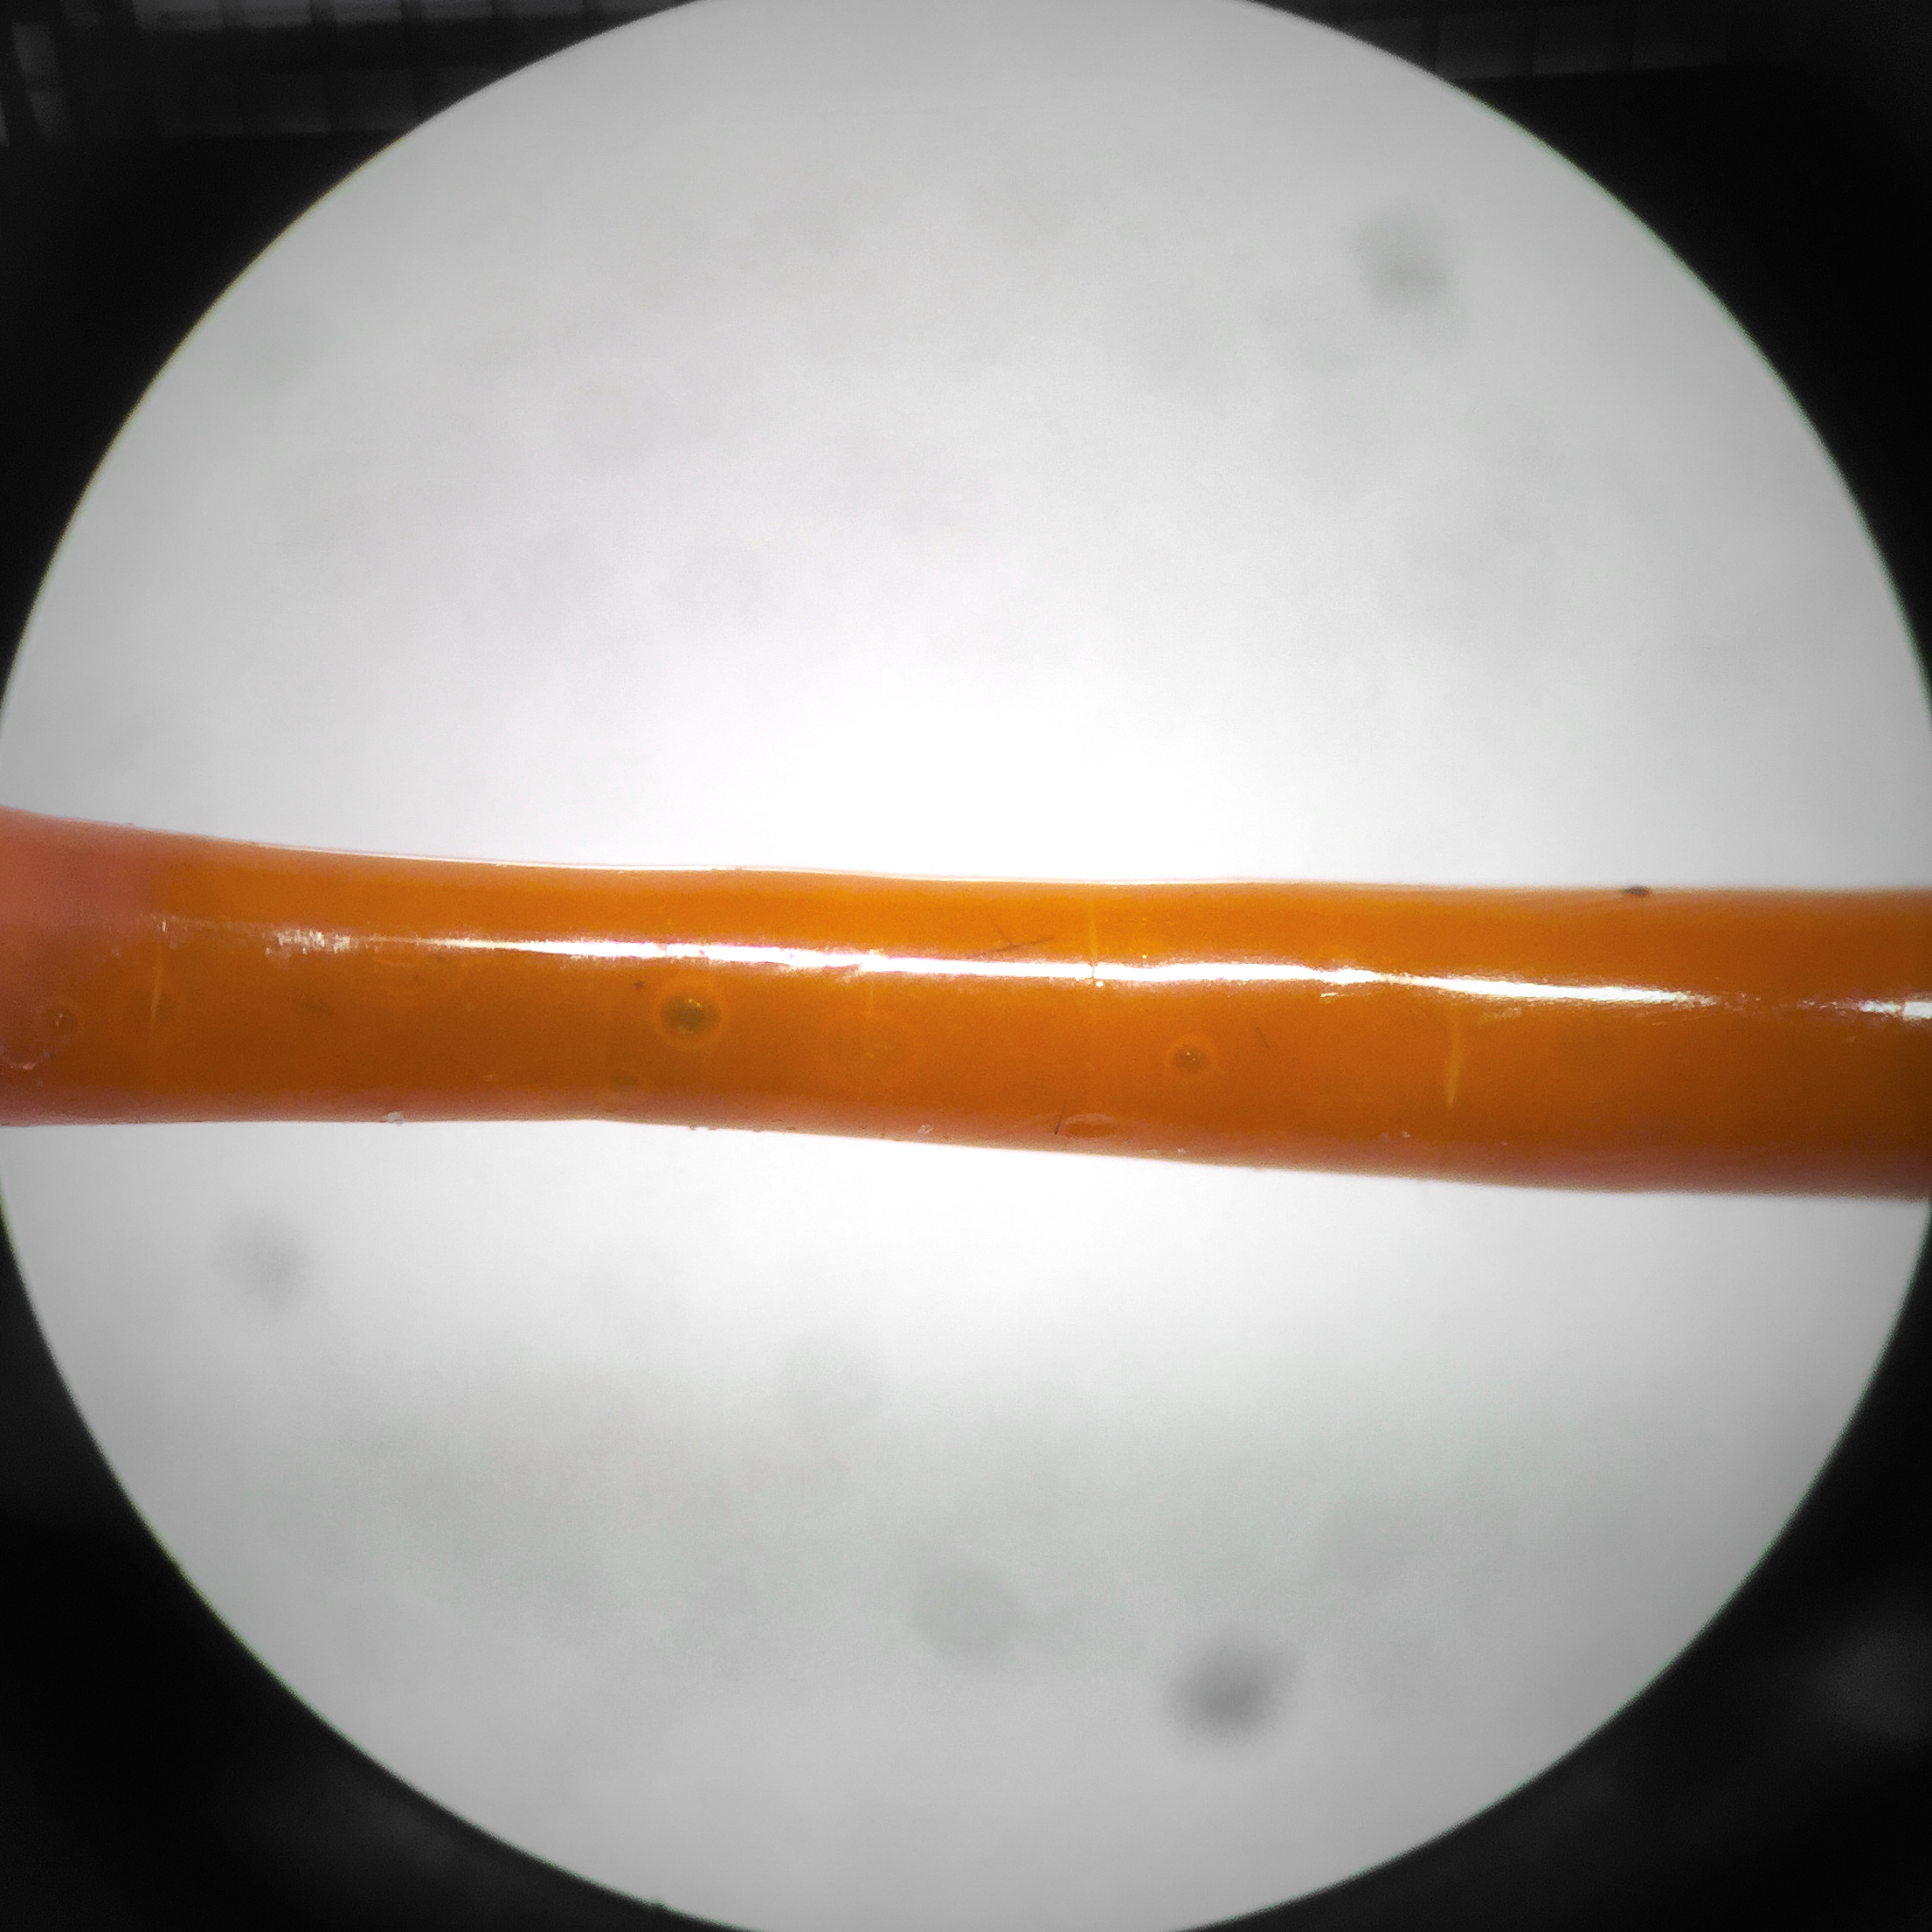
\includegraphics[width=\textwidth]{./figures/20-og-normal}
                \caption{Length normal.}
                \label{fig:20-og-normal}
        \end{subfigure}%
        ~ %add desired spacing between images, e. g. ~, \quad, \qquad, \hfill etc.
          %(or a blank line to force the subfigure onto a new line)
        \begin{subfigure}[b]{0.3\textwidth}
                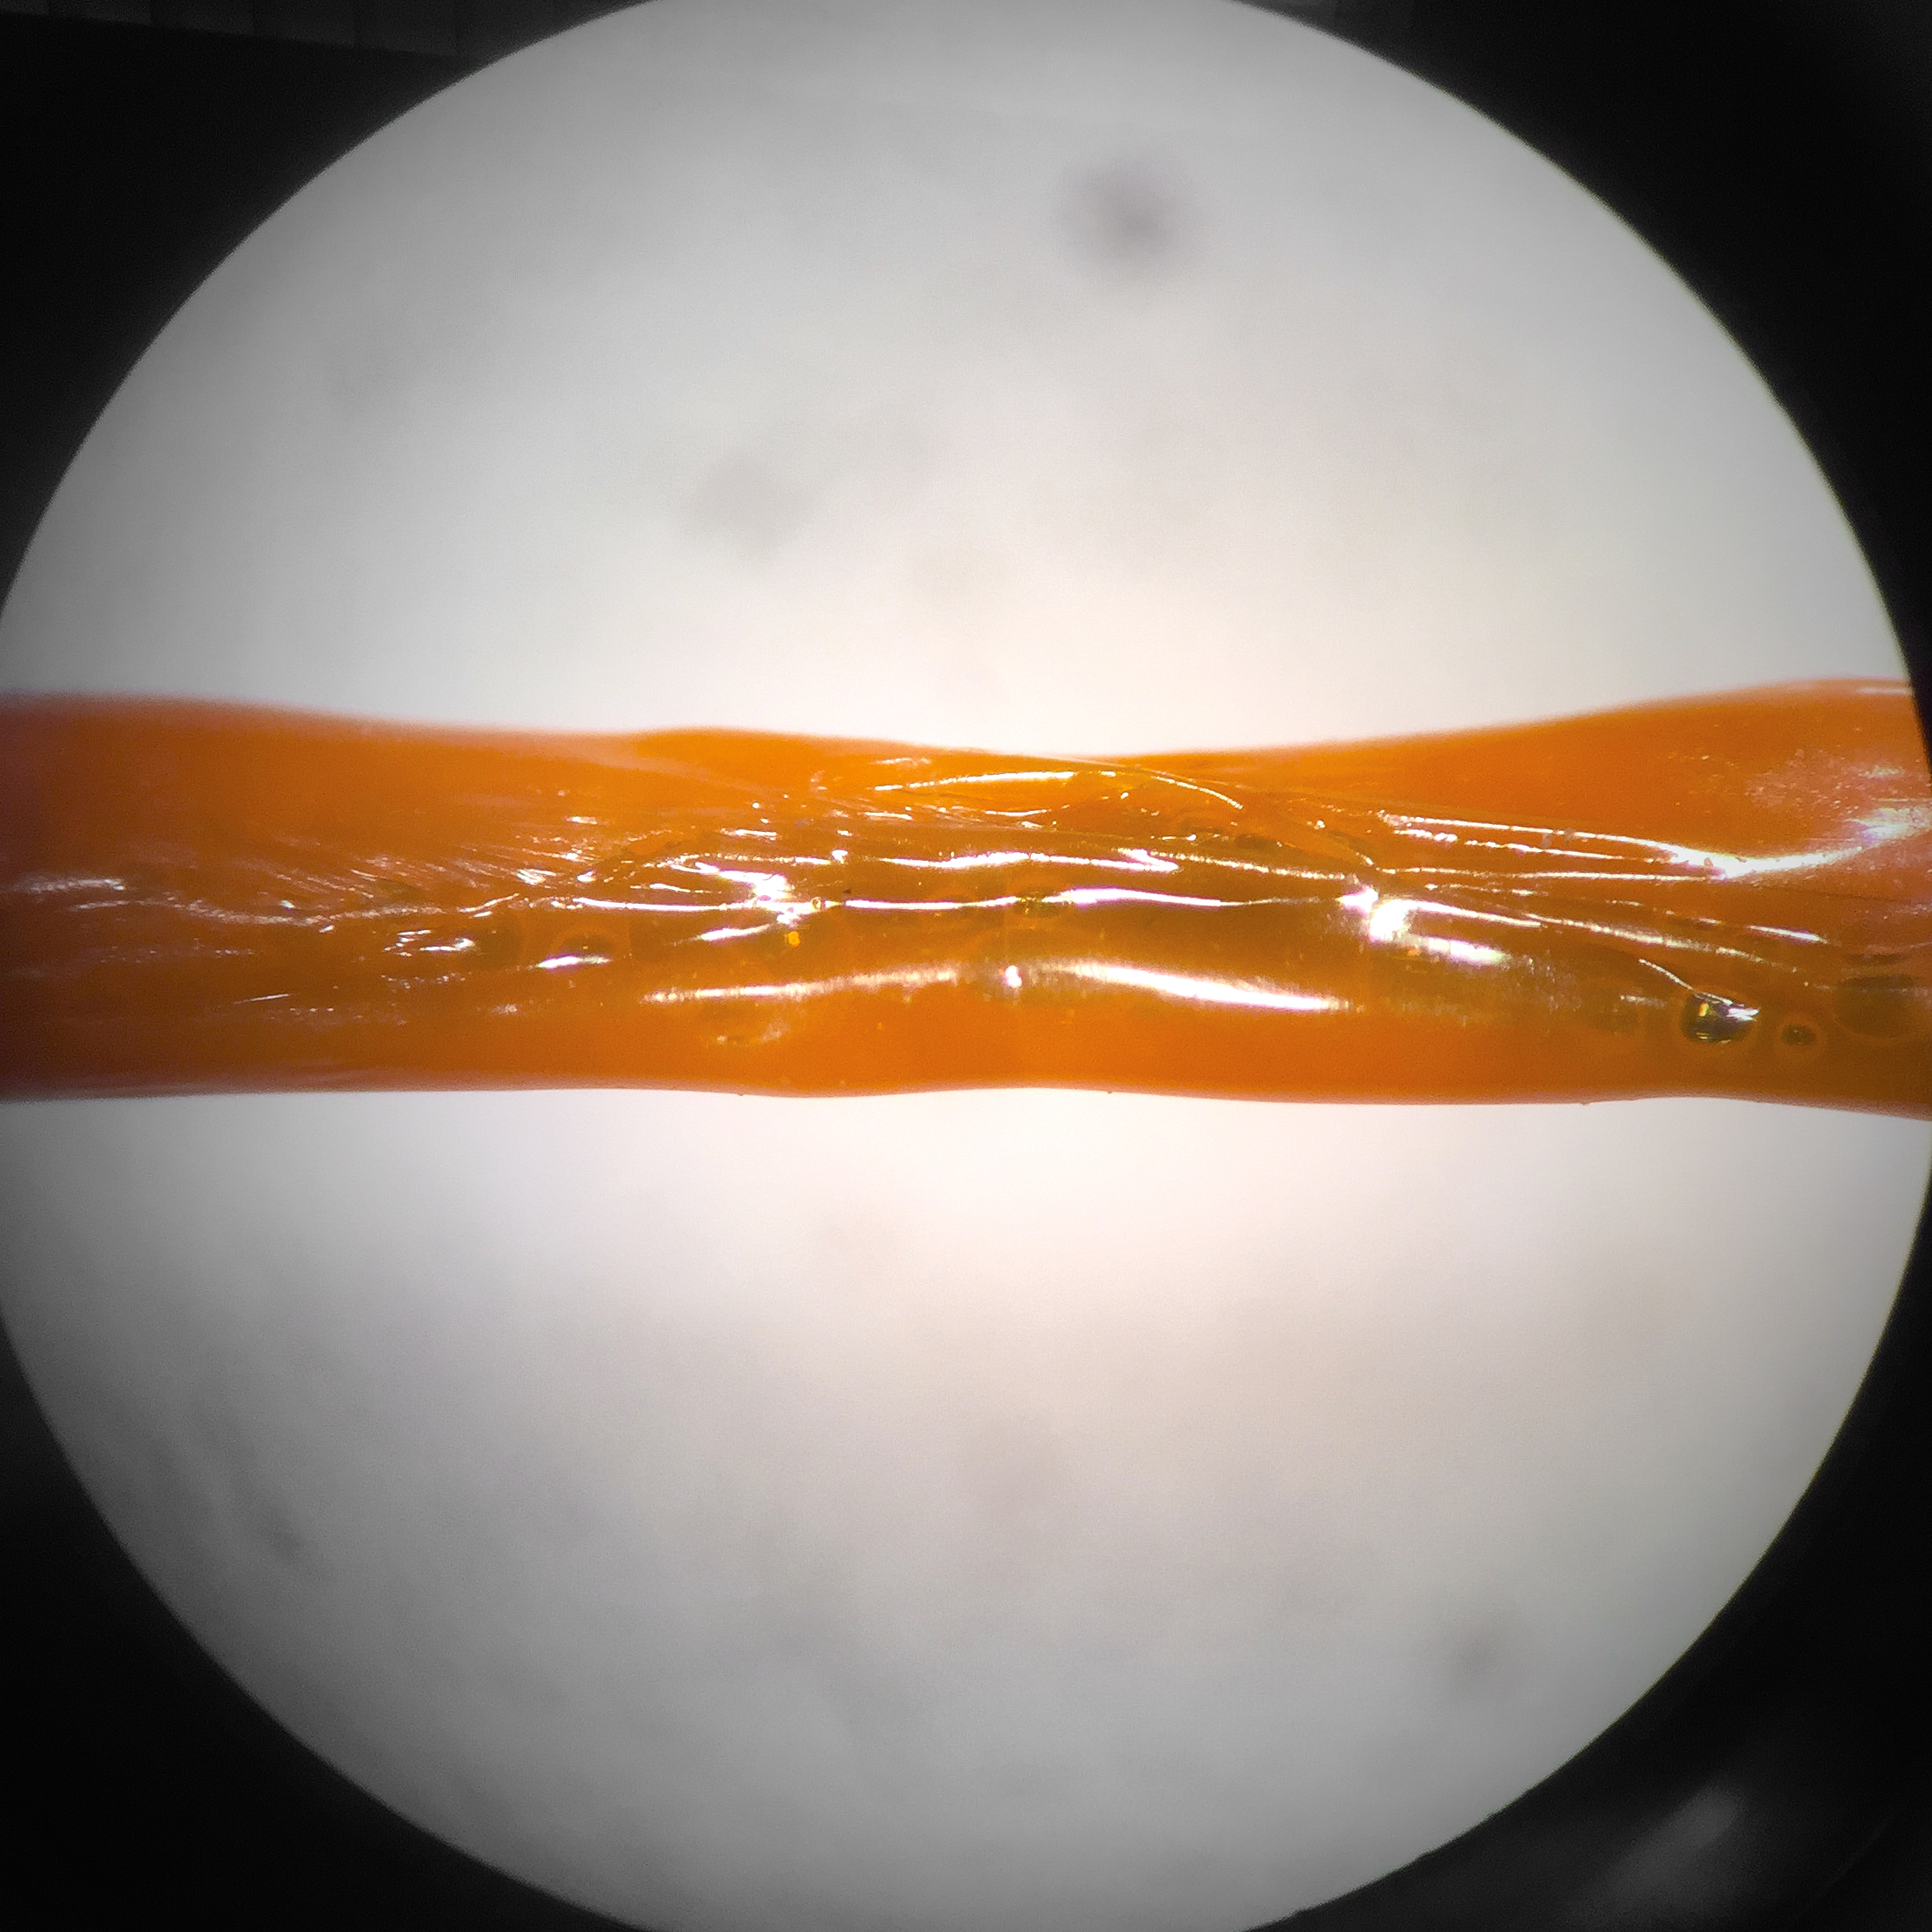
\includegraphics[width=\textwidth]{./figures/20-og-defect}
                \caption{Length defect.}
                \label{fig:20-og-defect}
        \end{subfigure}
        ~ %add desired spacing between images, e. g. ~, \quad, \qquad, \hfill etc.
          %(or a blank line to force the subfigure onto a new line)
        \begin{subfigure}[b]{0.3\textwidth}
                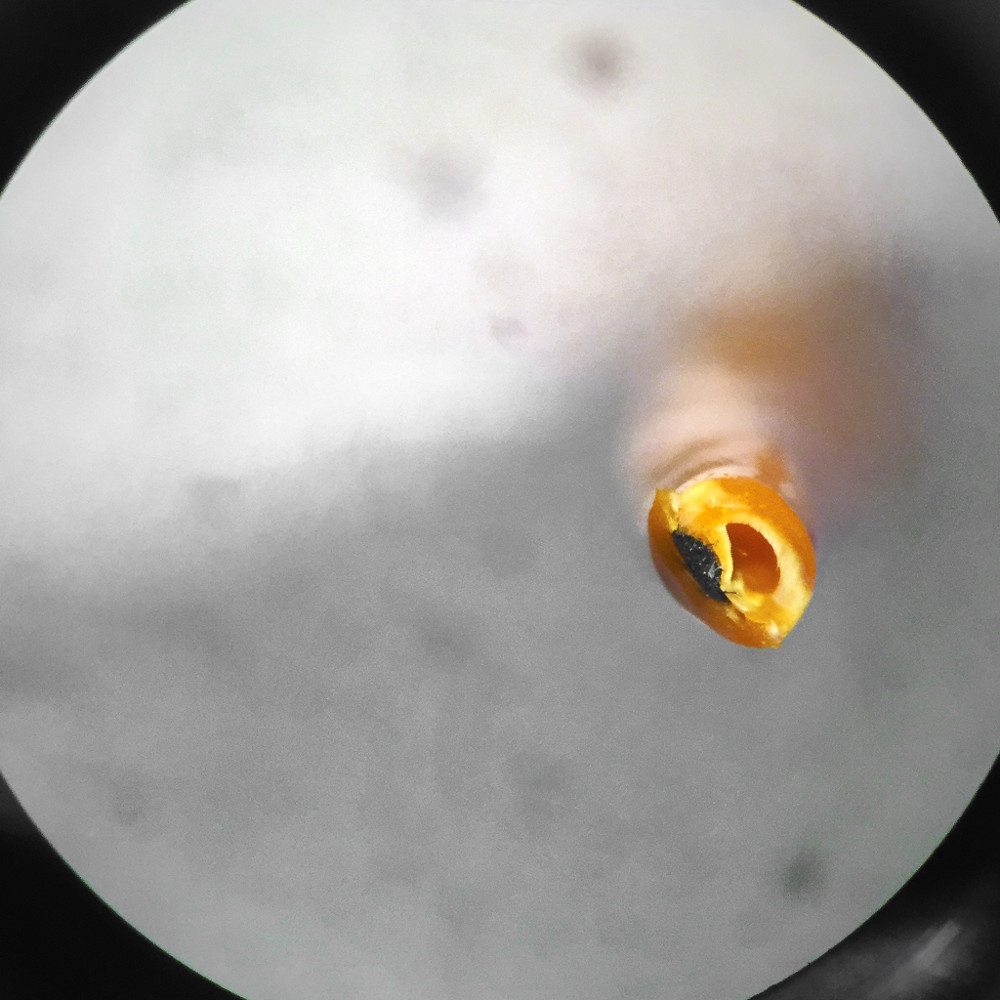
\includegraphics[width=\textwidth]{./figures/20-og-end}
                \caption{Cross section.}
                \label{fig:20-og-end}
        \end{subfigure}
        \caption{Microscopic views (10x) of a CFRP filament created with 20 dips using the partially immersed guide.}\label{fig:20-og}
\end{figure}

% inernal guide

\begin{figure}[h!]
        \centering
        \begin{subfigure}[b]{0.3\textwidth}
                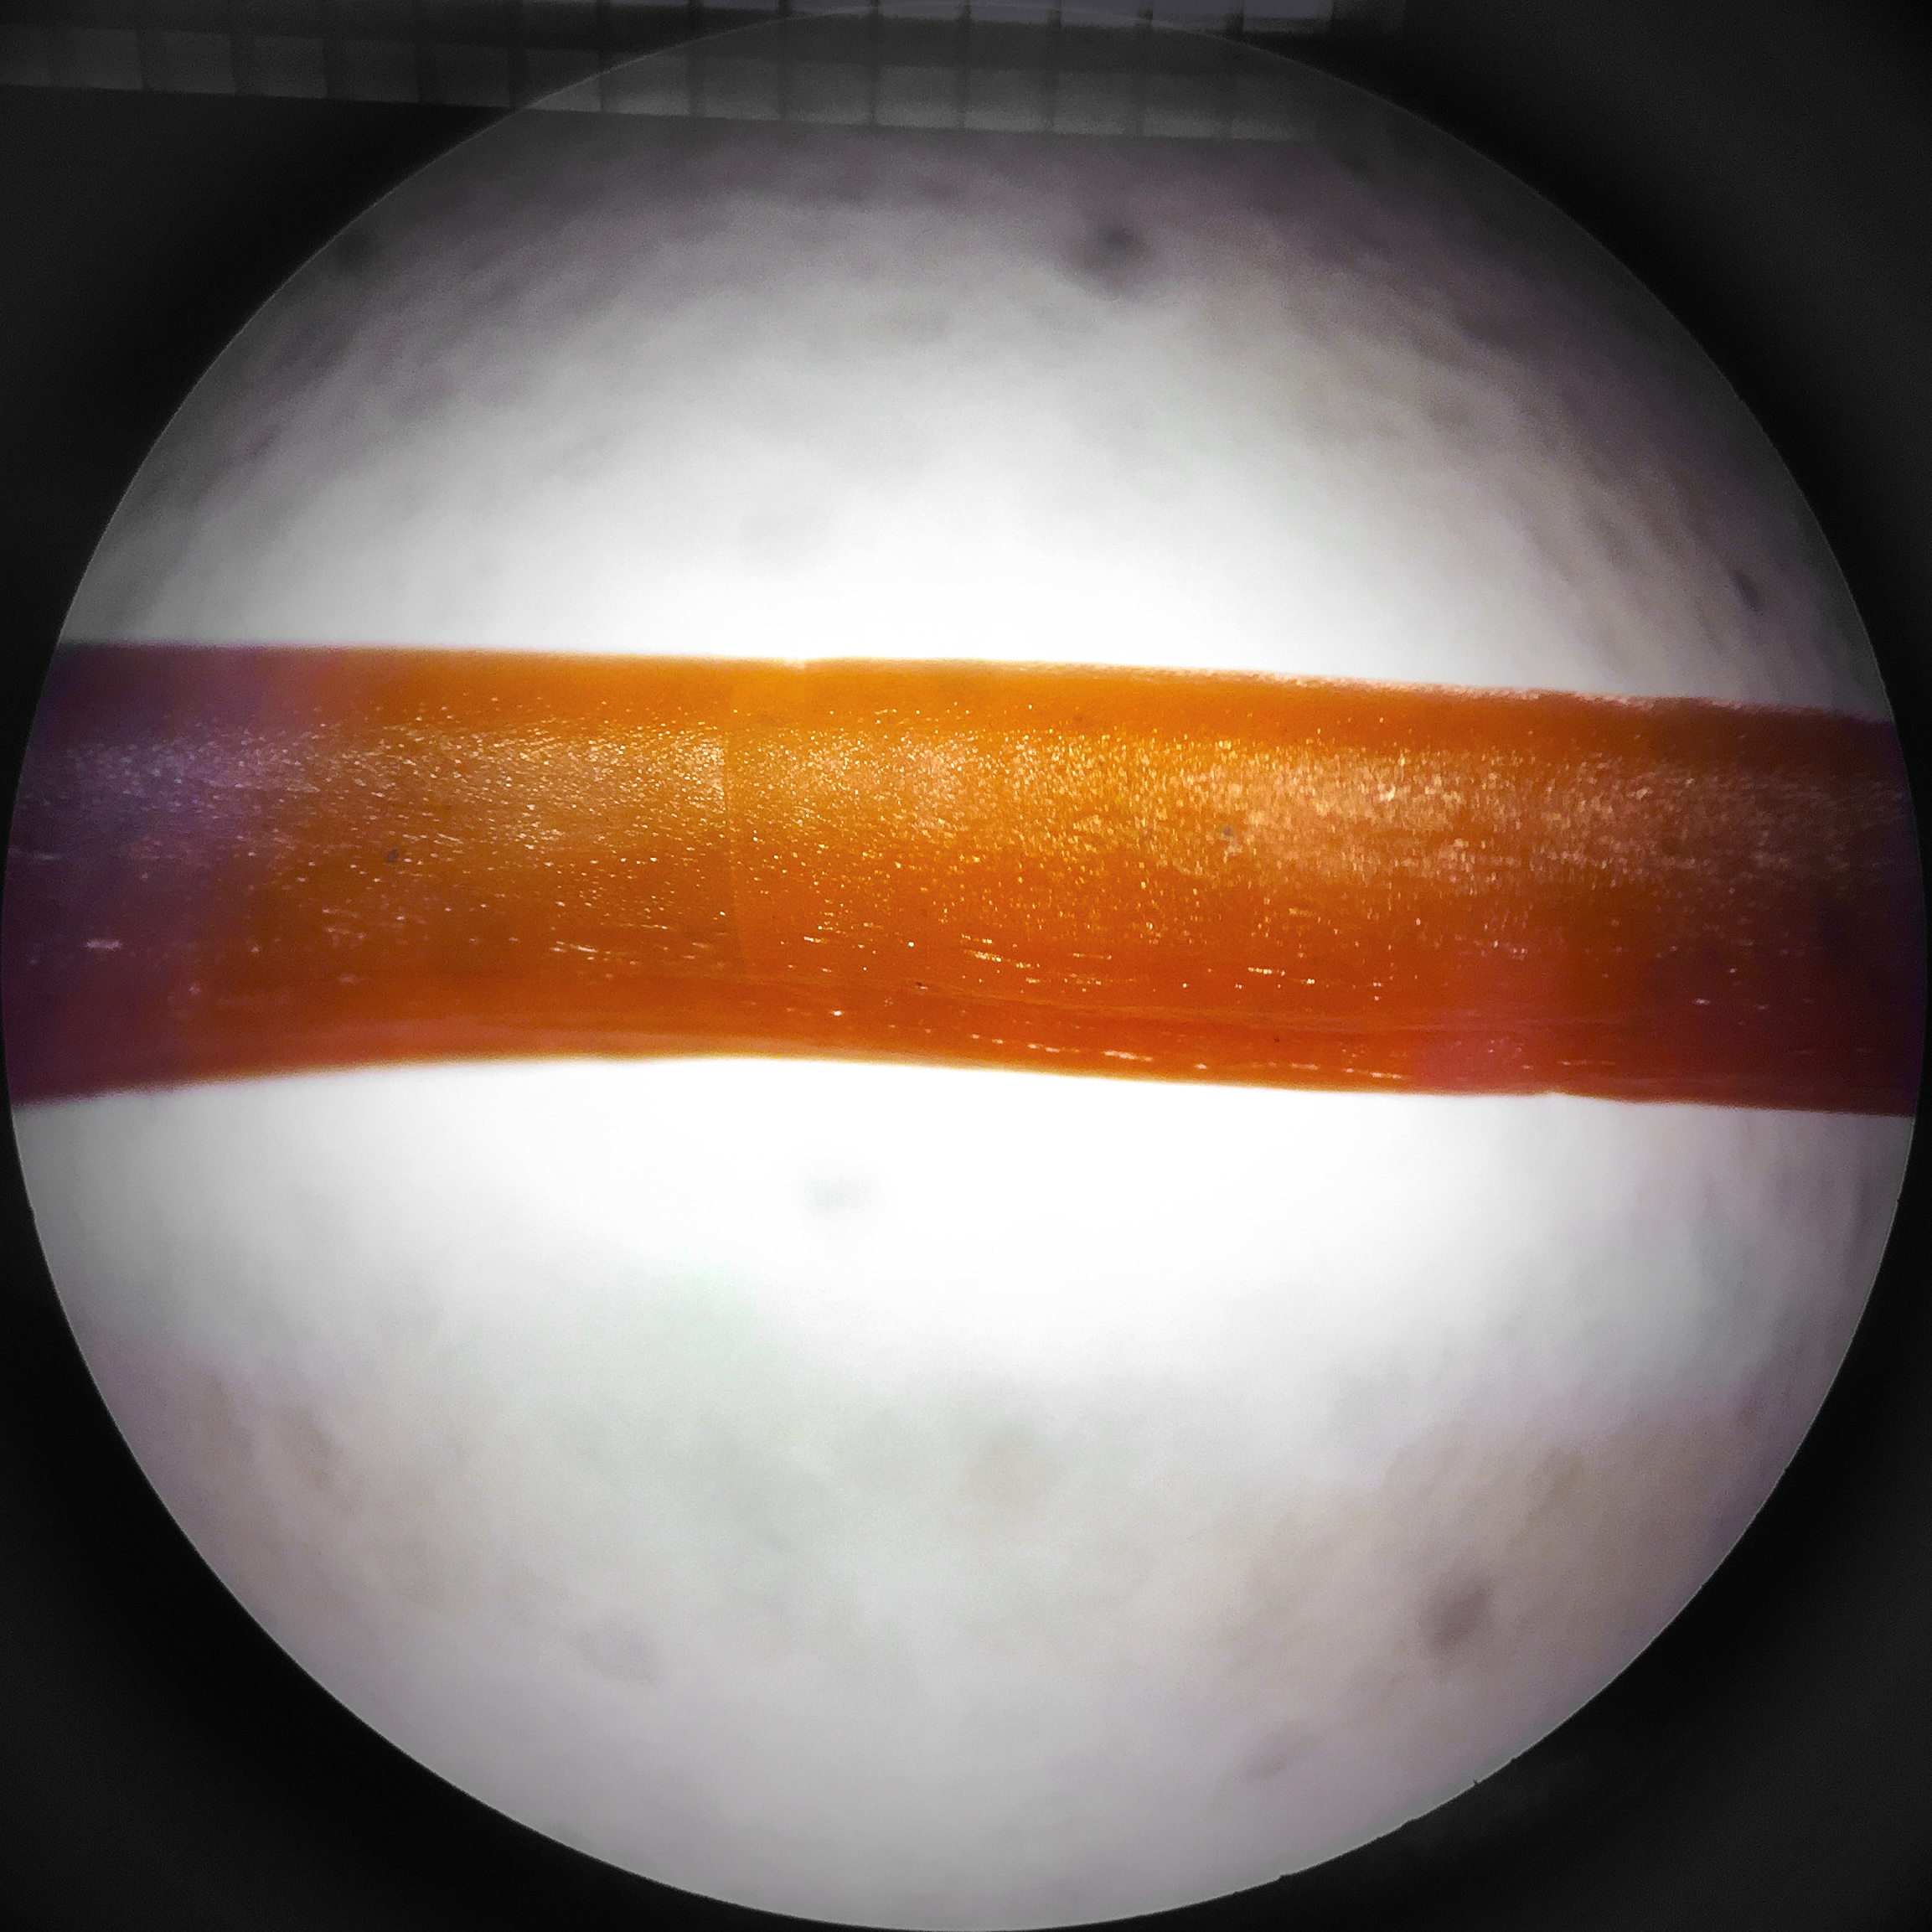
\includegraphics[width=\textwidth]{./figures/20-ng-normal}
                \caption{Length normal.}
                \label{fig:20-og-normal}
        \end{subfigure}%
        ~ %add desired spacing between images, e. g. ~, \quad, \qquad, \hfill etc.
          %(or a blank line to force the subfigure onto a new line)
        \begin{subfigure}[b]{0.3\textwidth}
                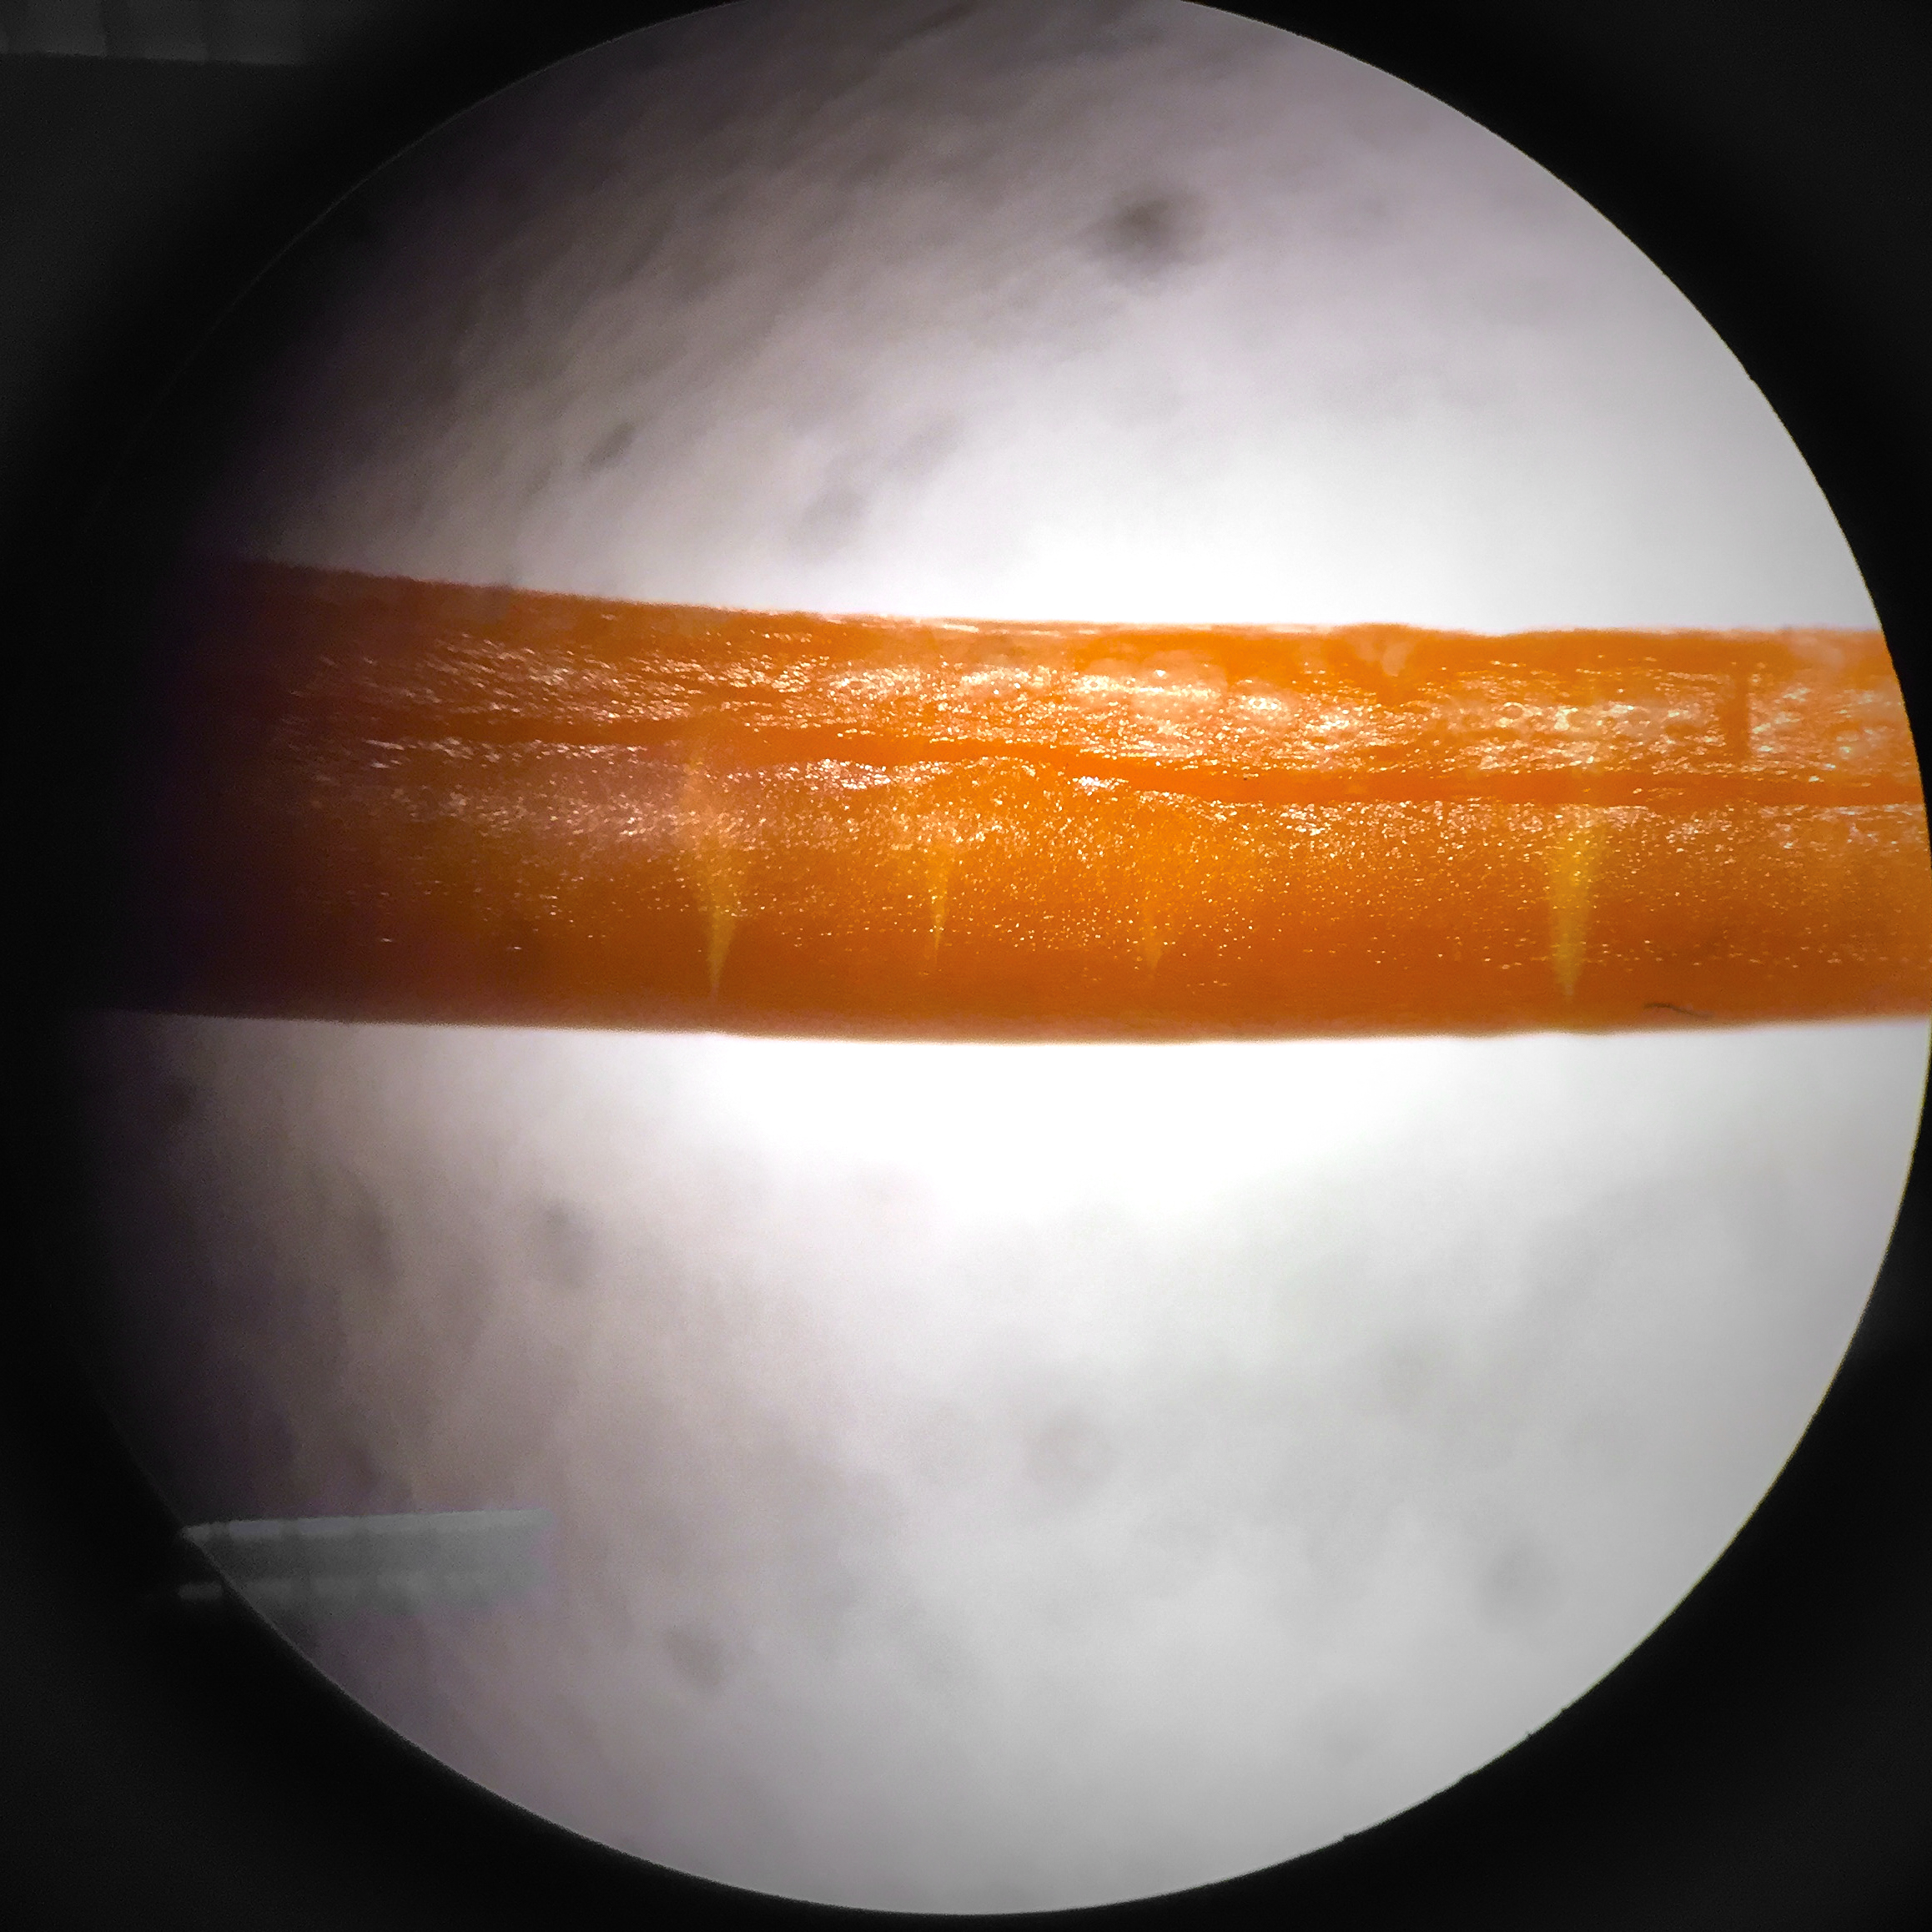
\includegraphics[width=\textwidth]{./figures/20-ng-defect}
                \caption{Length defect.}
                \label{fig:20-og-defect}
        \end{subfigure}
        ~ %add desired spacing between images, e. g. ~, \quad, \qquad, \hfill etc.
          %(or a blank line to force the subfigure onto a new line)
        \begin{subfigure}[b]{0.3\textwidth}
                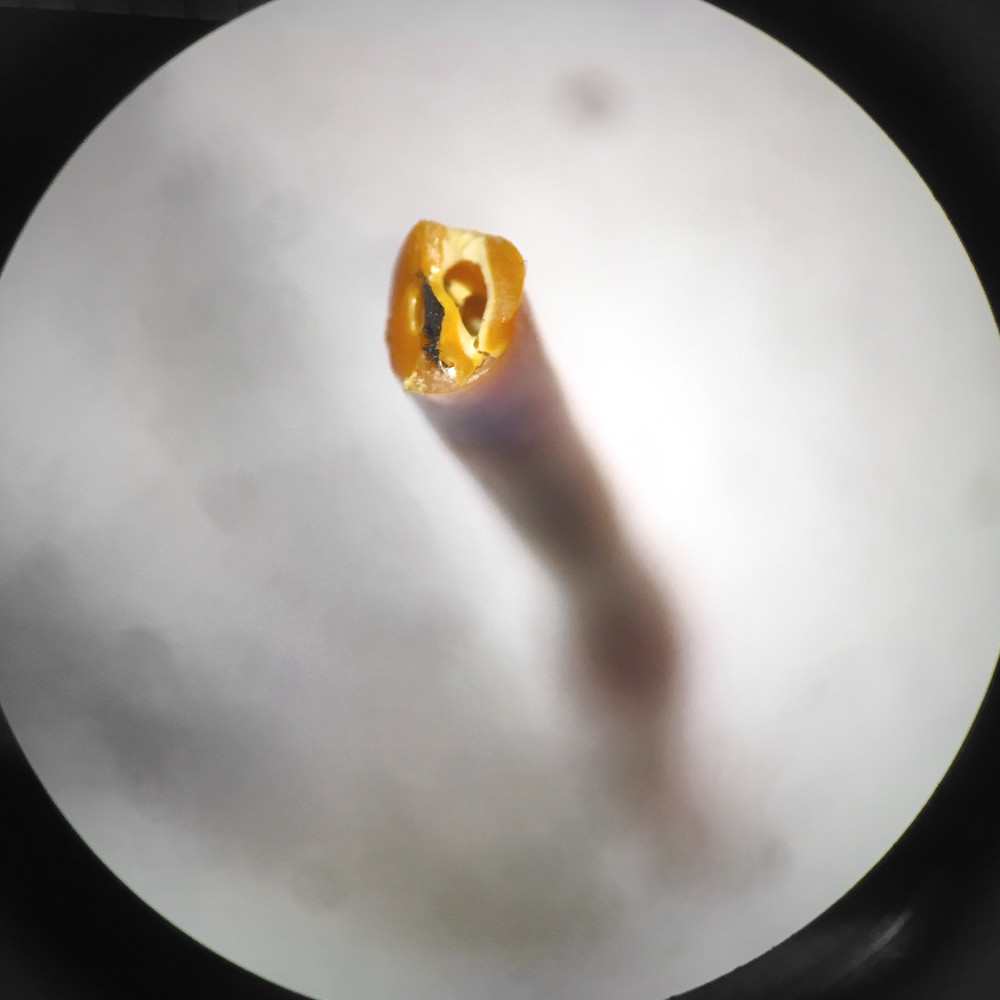
\includegraphics[width=\textwidth]{./figures/20-ng-end}
                \caption{Cross section.}
                \label{fig:20-og-end}
        \end{subfigure}
        \caption{Microscopic views (10x) of a CFRP filament created with 20 dips using the fully immersed guide.}\label{fig:20-ng}
\end{figure}

% 108 40 dip

\begin{figure}[h!]
        \centering
        \begin{subfigure}[b]{0.3\textwidth}
                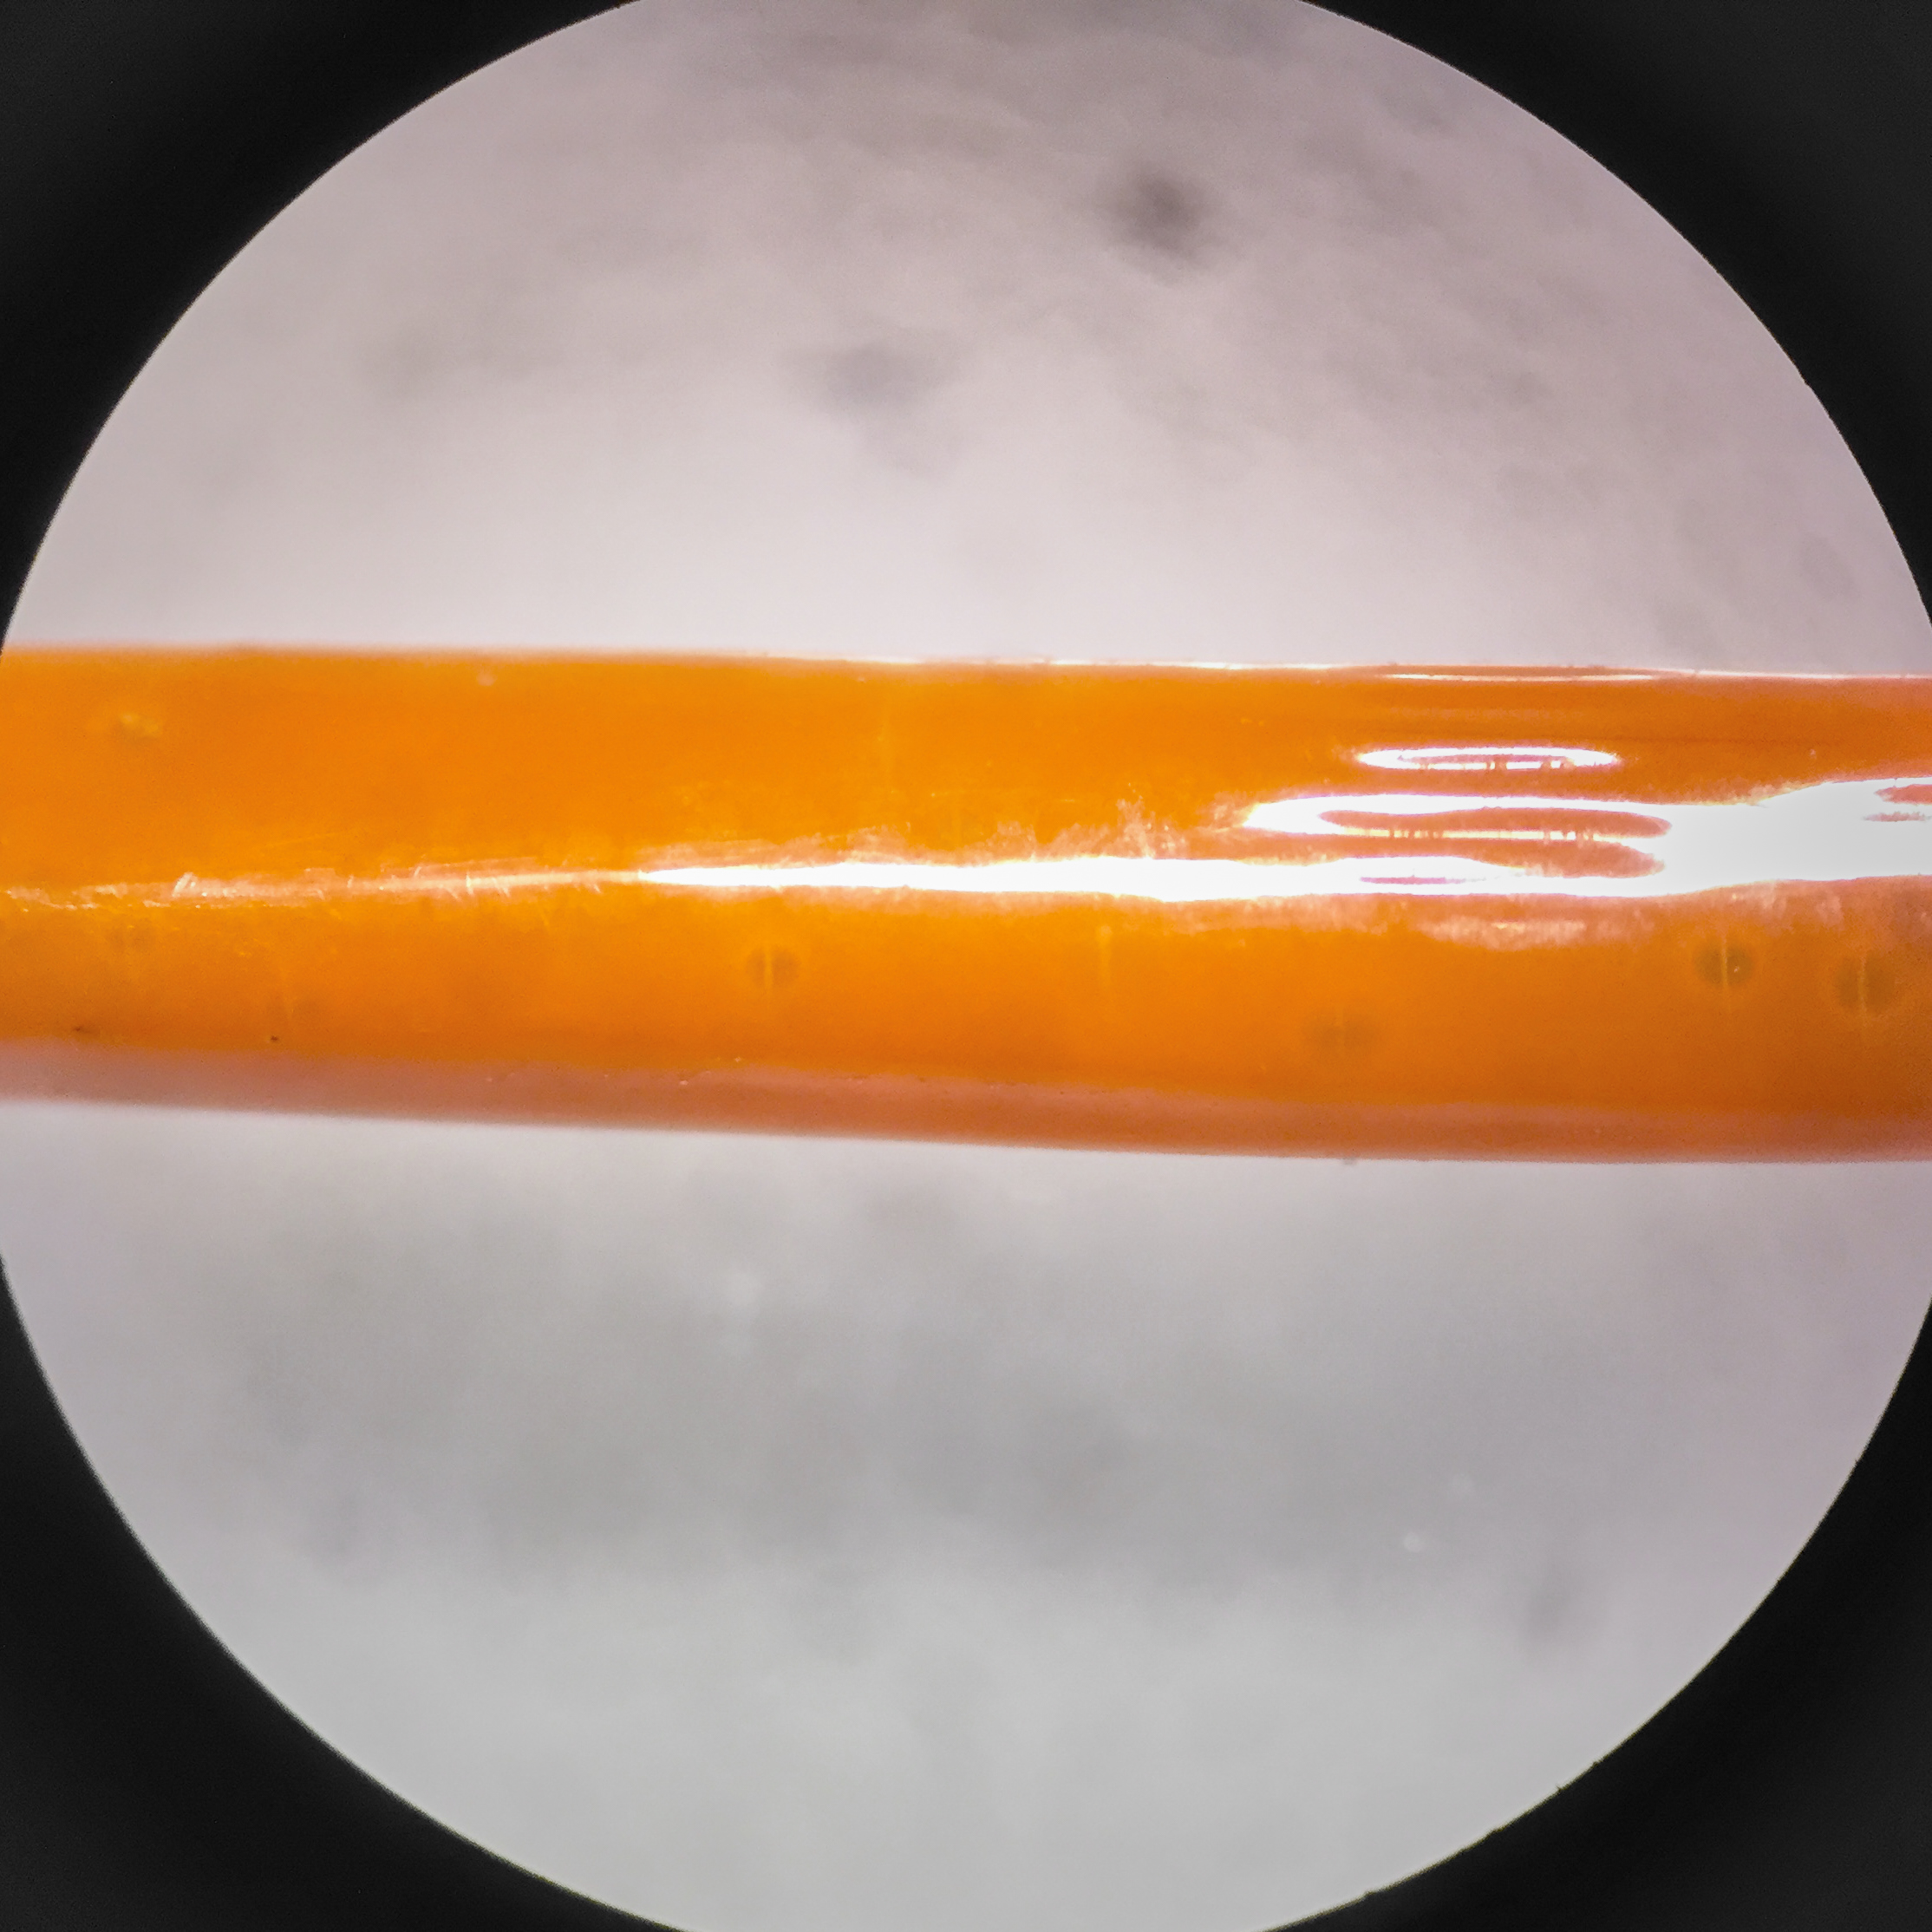
\includegraphics[width=\textwidth]{./figures/filament-108-40-dip-side}
                \caption{Length.}
                \label{fig:filament-108-40-dip-side}
        \end{subfigure}
        \begin{subfigure}[b]{0.3\textwidth}
                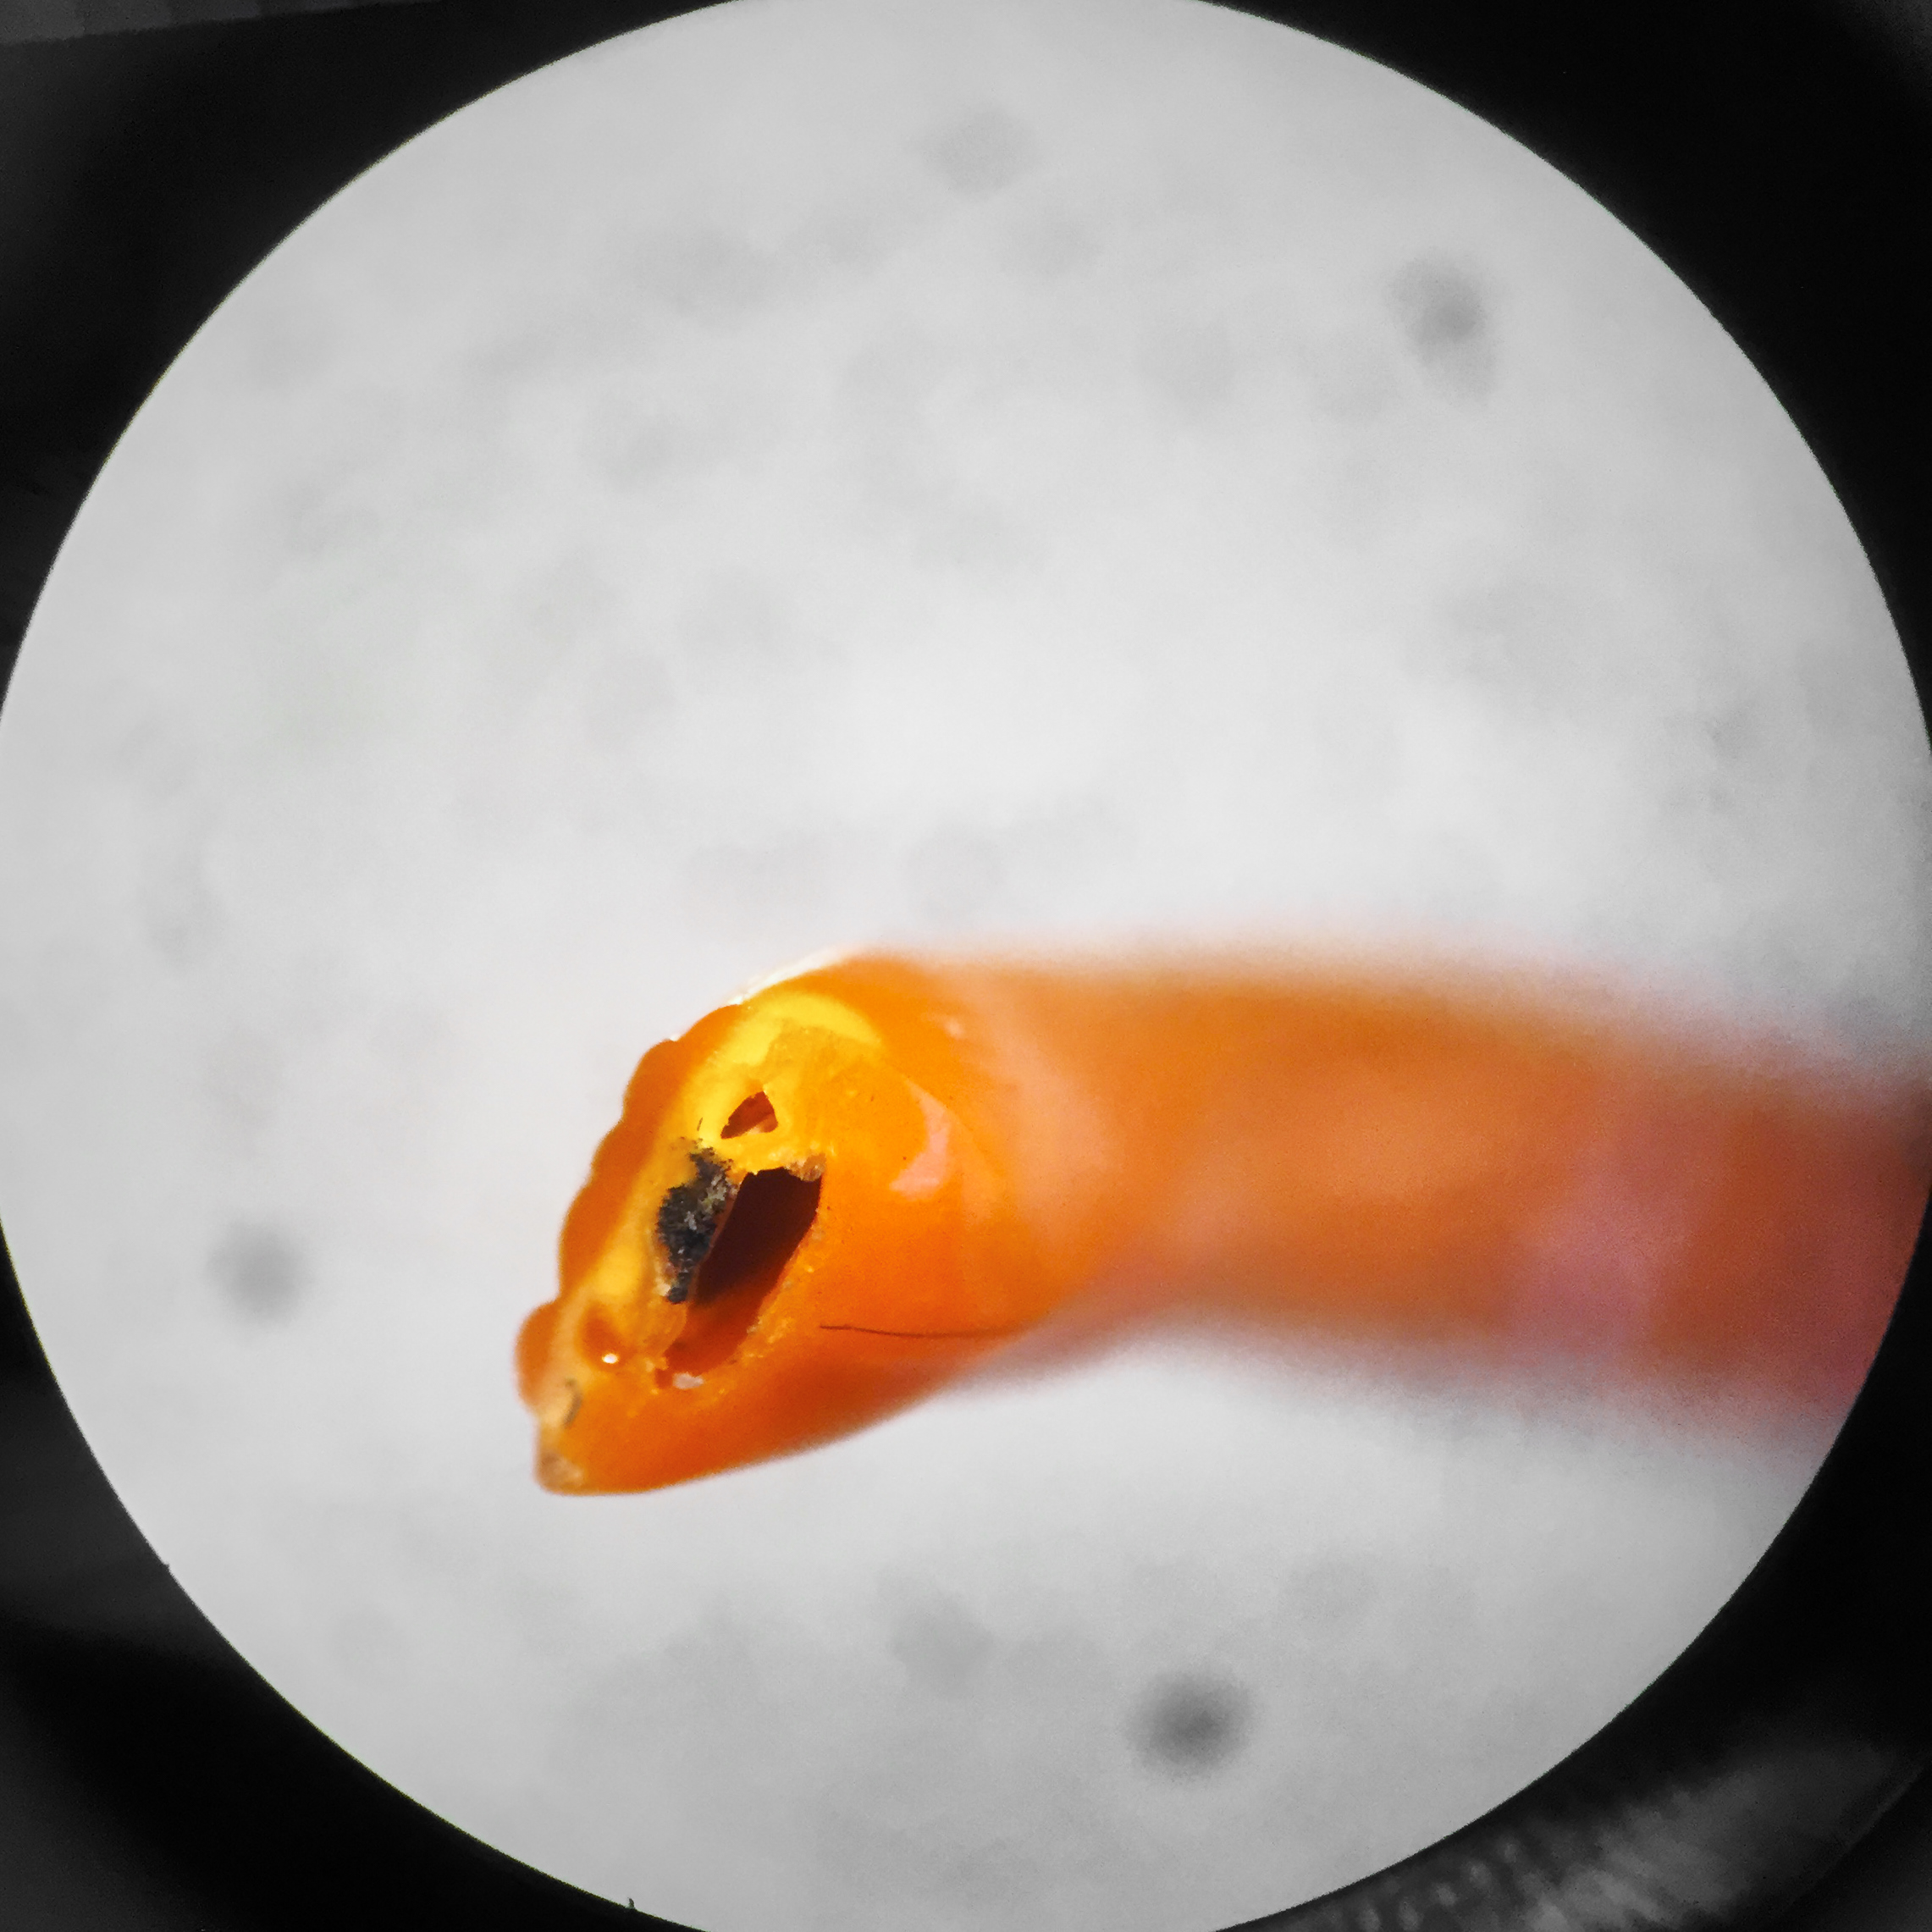
\includegraphics[width=\textwidth]{./figures/filament-108-40-dip-end}
                \caption{Cross section.}
                \label{fig:filament-108-40-dip-end}
        \end{subfigure}
        \caption{Microscopic views (10x) of a CFRP filament created with 10 dips using the fully immersed guide in a 4\% ABS solution.}\label{fig:filament-108-40-dip-microscope}
\end{figure}

% 108 40 bath

\begin{figure}[h!]
        \centering
        \begin{subfigure}[b]{0.3\textwidth}
                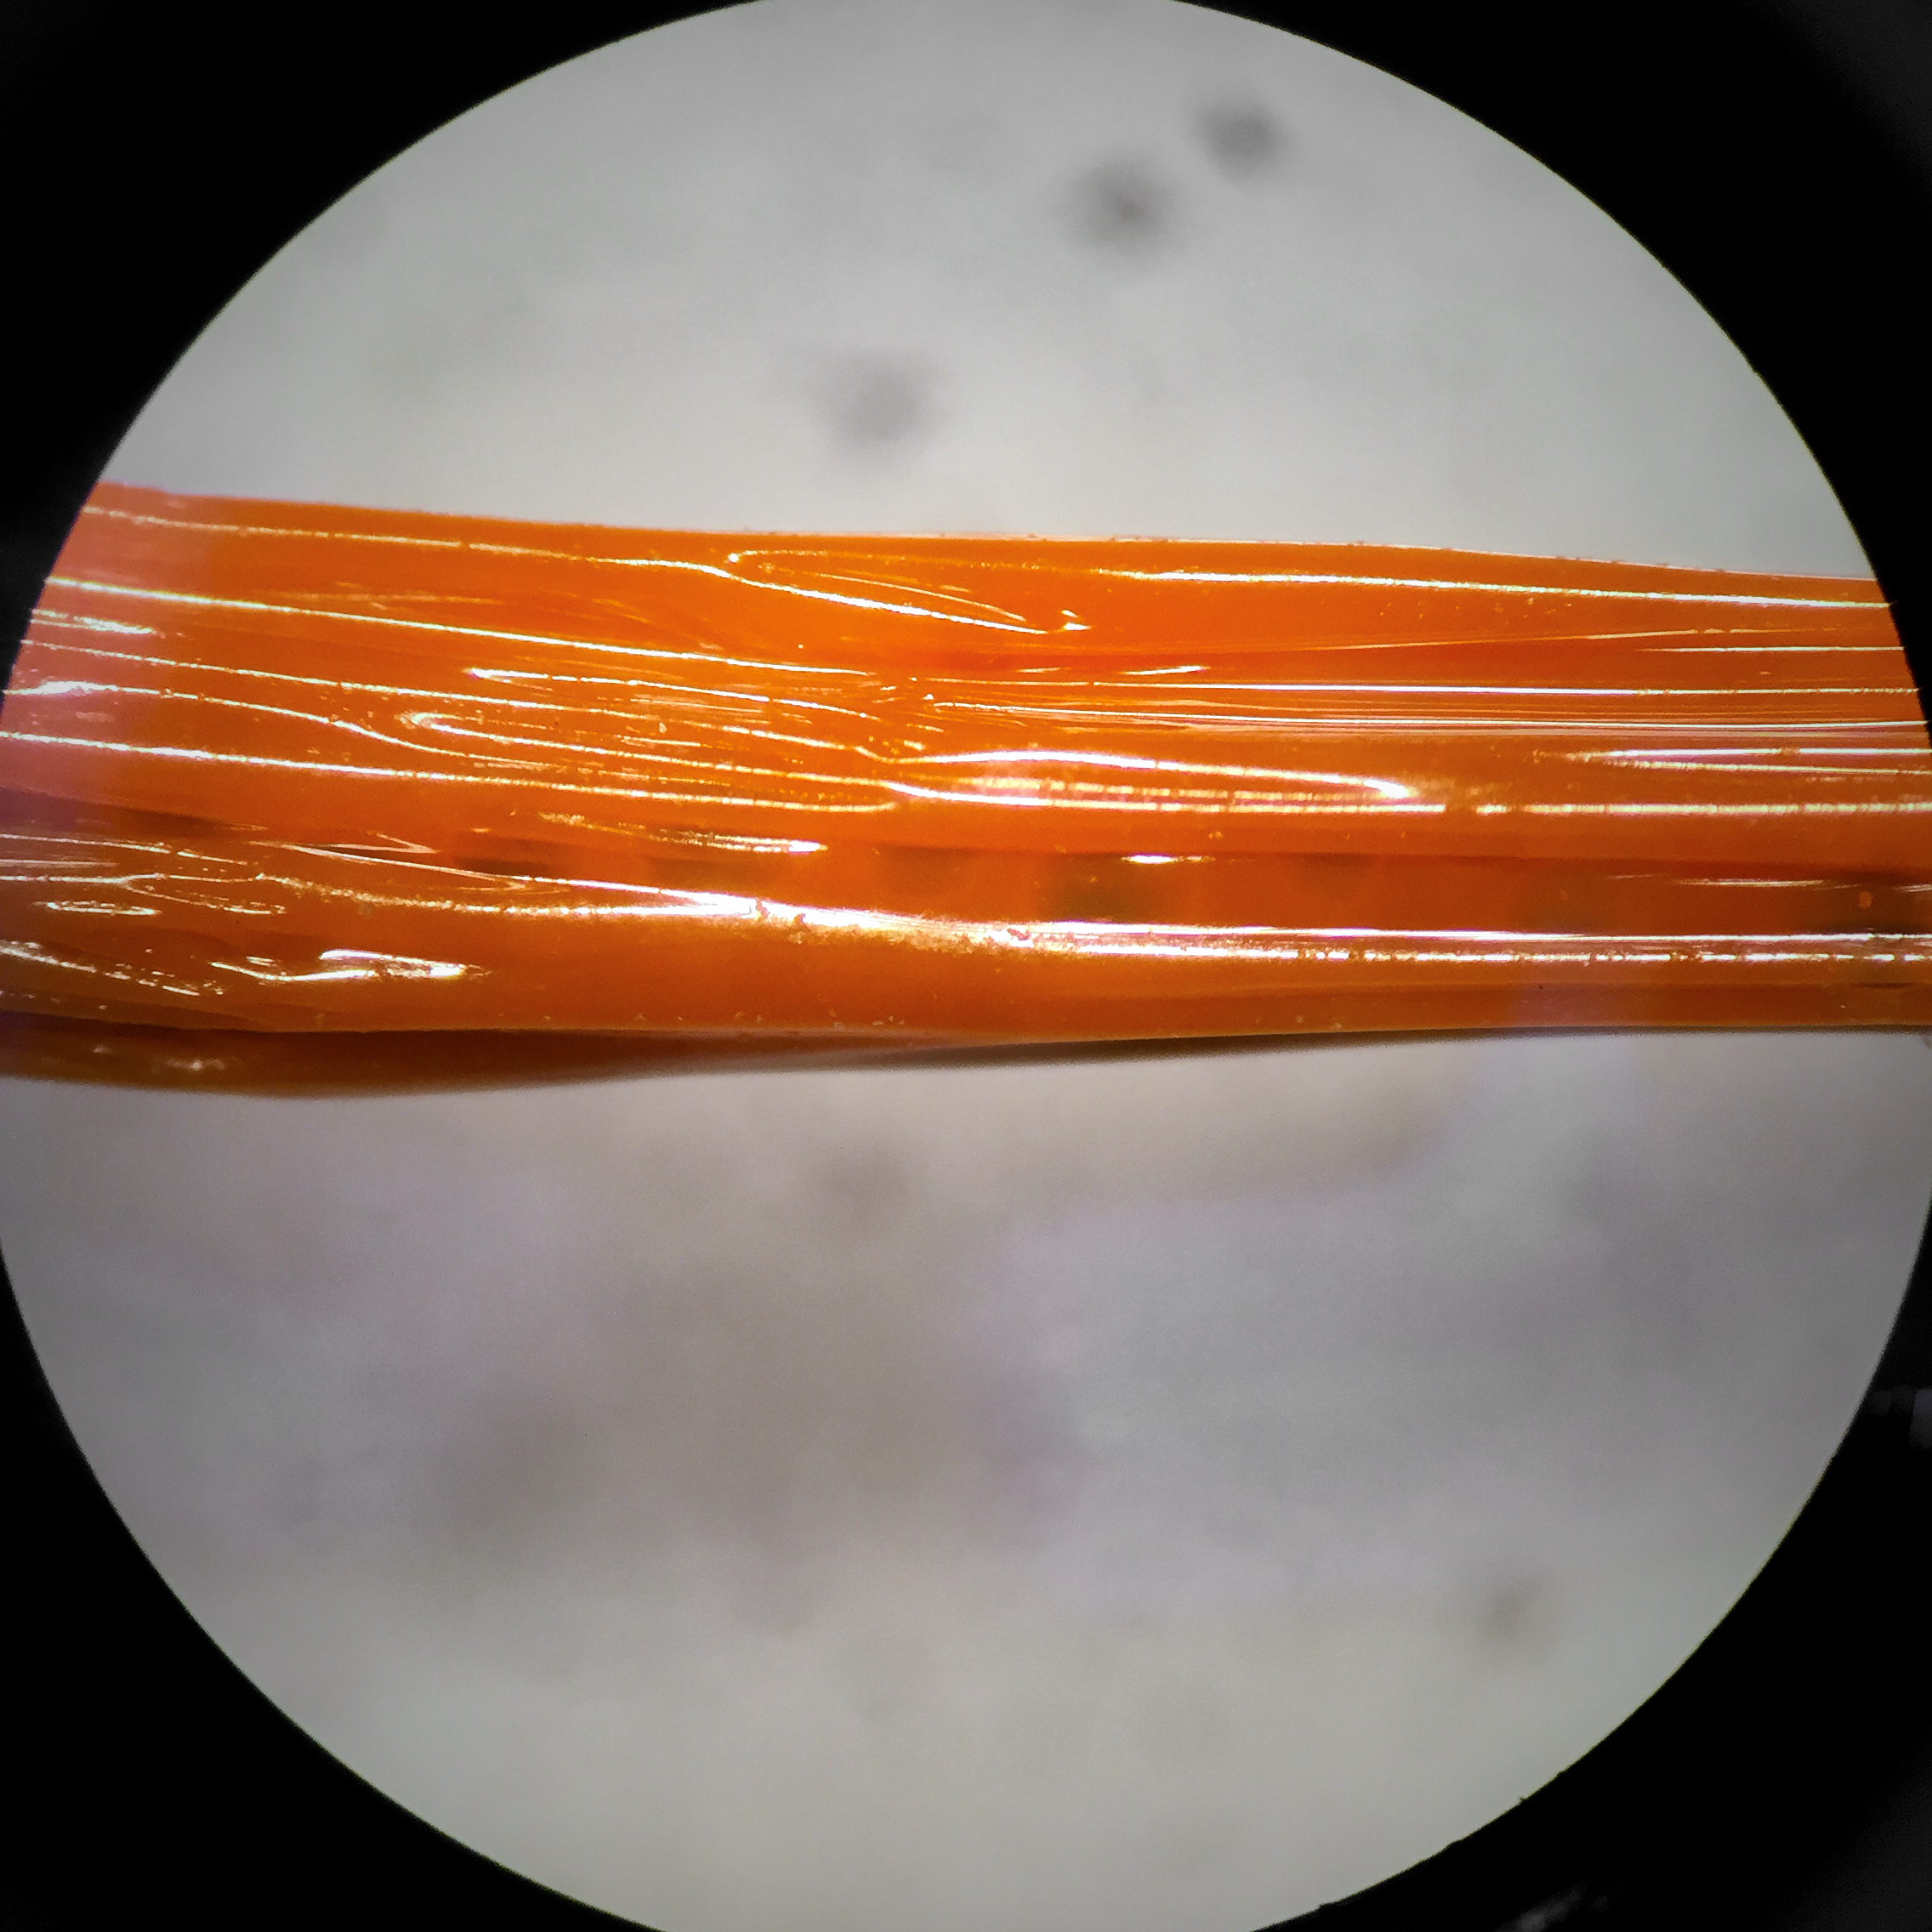
\includegraphics[width=\textwidth]{./figures/filament-108-40-flat-side}
                \caption{Length.}
                \label{fig:filament-108-40-flat-side}
        \end{subfigure}
        \begin{subfigure}[b]{0.3\textwidth}
                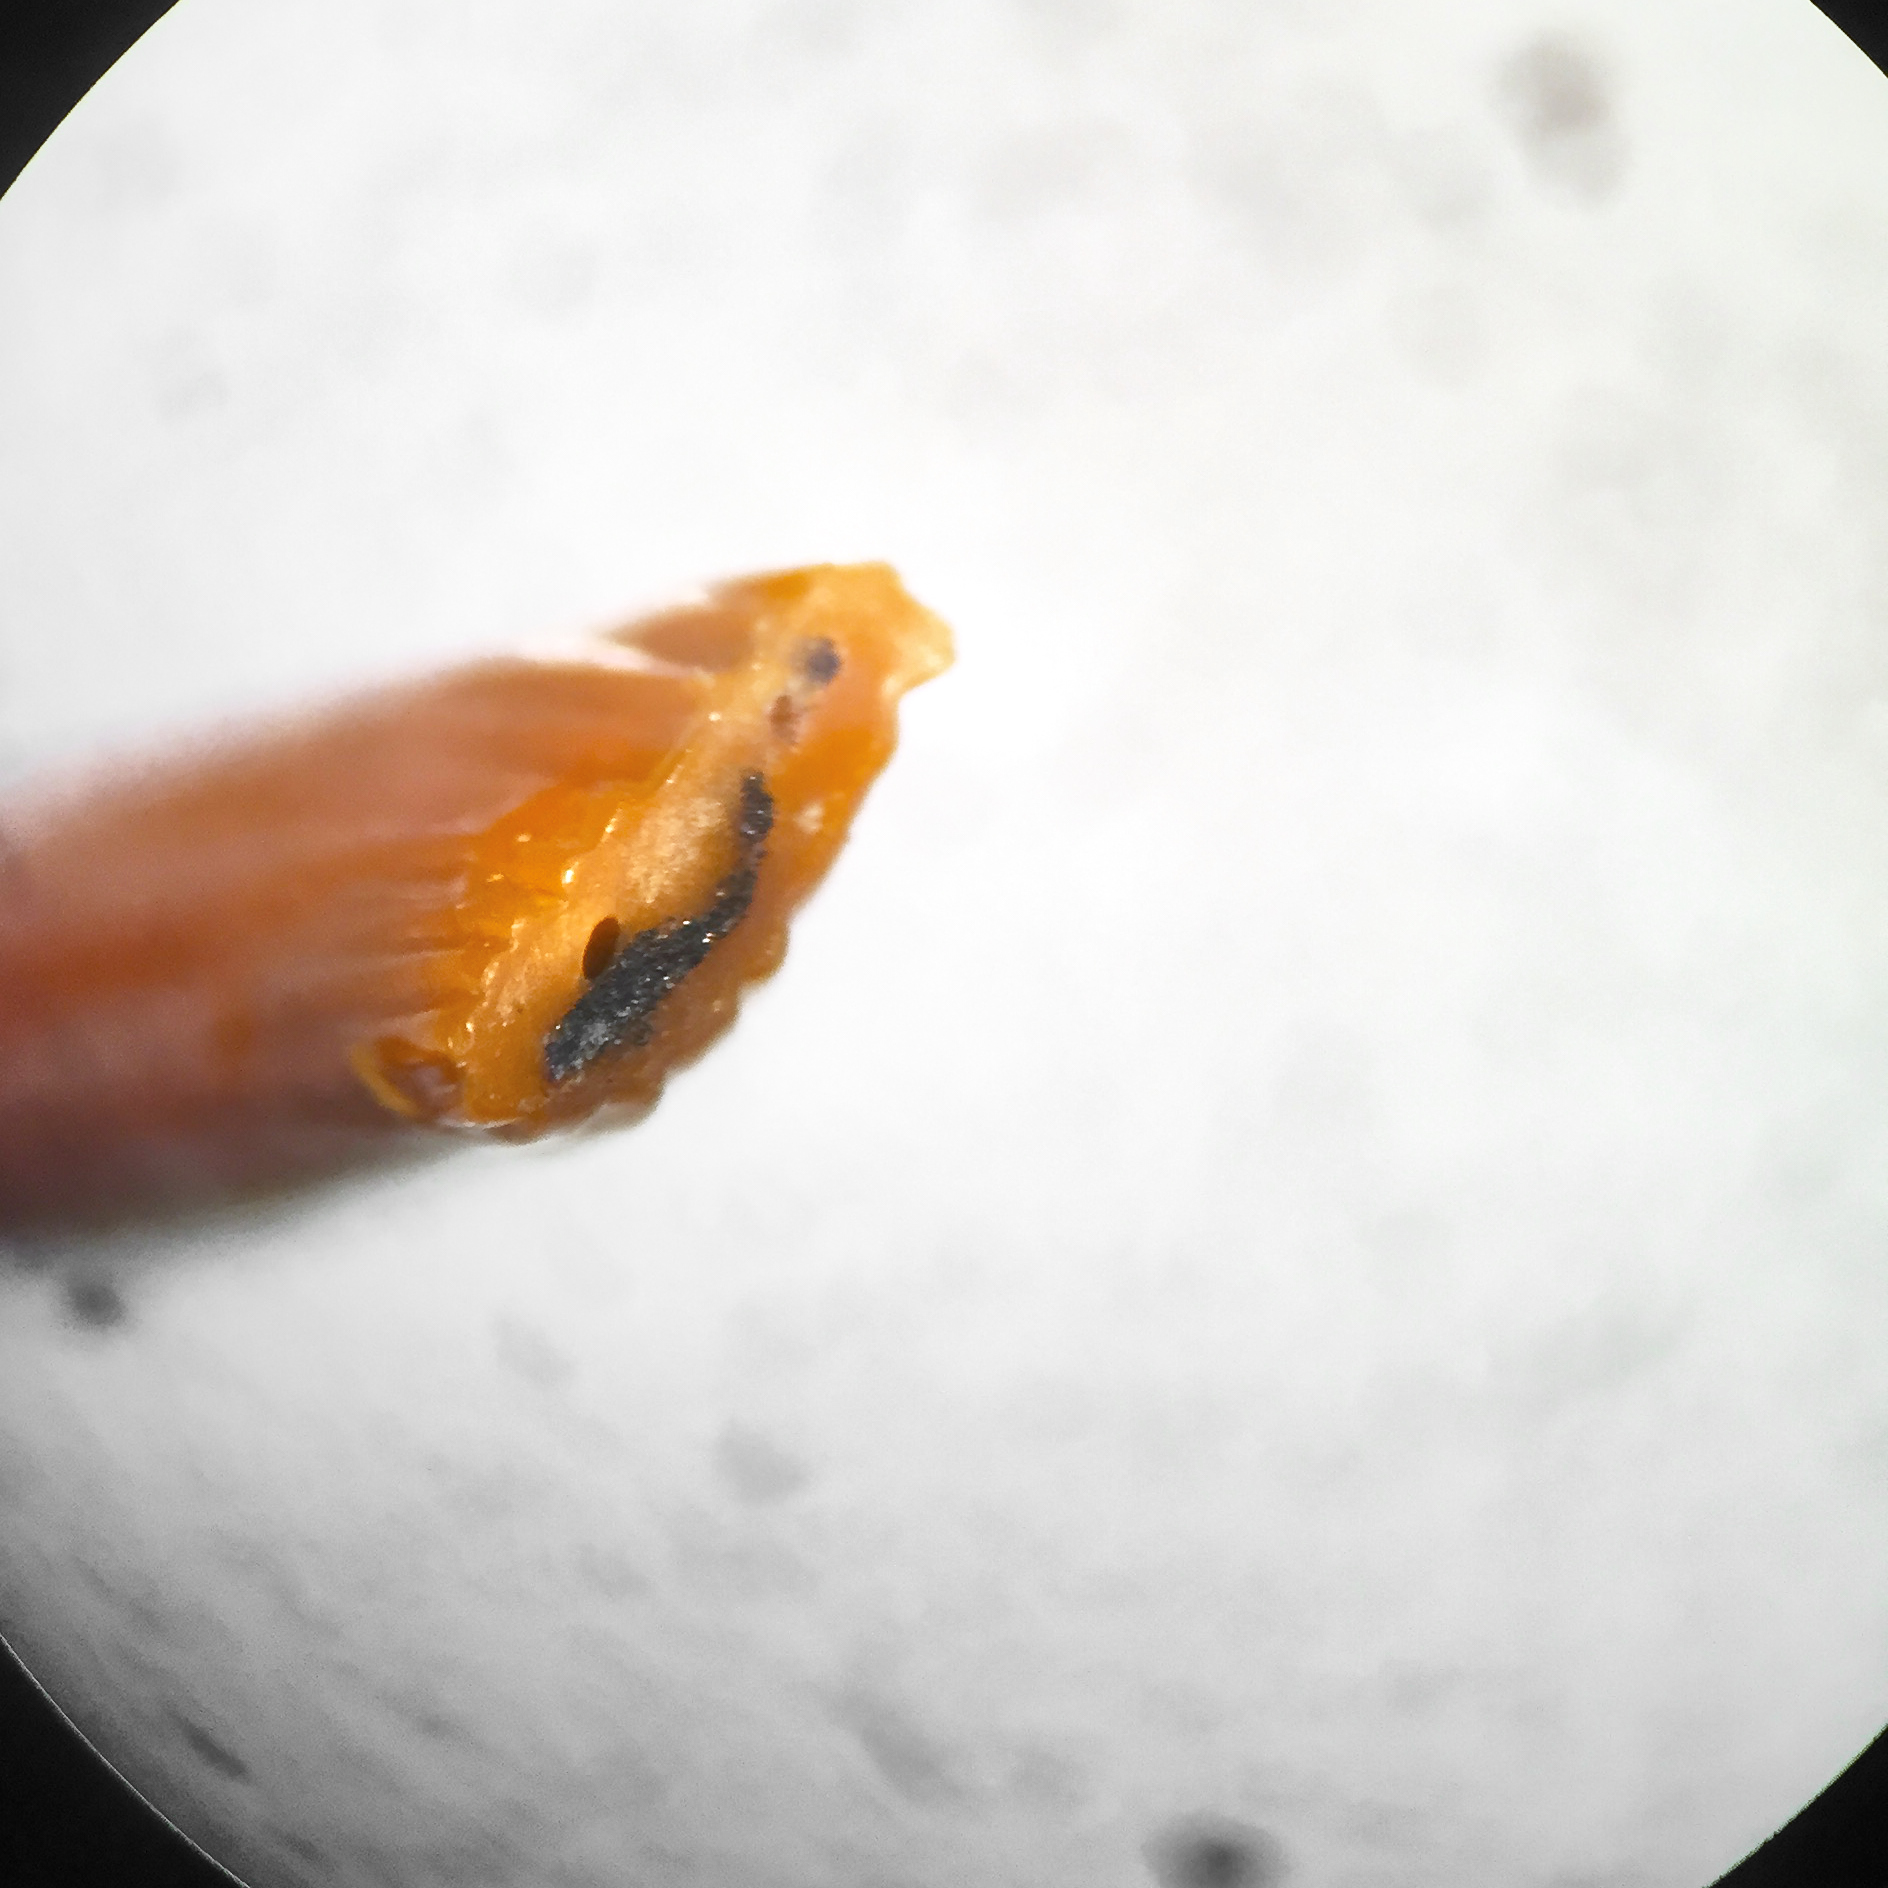
\includegraphics[width=\textwidth]{./figures/filament-108-40-flat-end}
                \caption{Cross section.}
                \label{fig:filament-108-40-flat-end}
        \end{subfigure}
        \caption{Microscopic views (10x) of a CFRP filament created with 5 bathing rotations in a 5\% ABS solution.}\label{fig:filament-108-40-bath-microscope}
\end{figure}


%%% Dipping Results Summary

\begin{table}[h!]
    \centering
    \begin{tabular}{p{1.5in}|p{1in}|p{0.75in}|p{0.75in}|p{0.75in}|p{0.75in}}
        Filament Formulation & Concentration of ABS, $m^3/m^3$ & Density, $kg/m^3$ & Percent Carbon Fiber, $kg/kg$ & Filament Diameter, $mm$ & ABS Added per Dip per Length, $kg/m$  \\ \hline \hline
        60 \textit{in} ABS, 40 \textit{mL} Acetone, Guided & 0.09 & 818 & 19 & 0.73 & 0.017 \\ \hline
        108 \textit{in} ABS, 40 \textit{mL} Acetone, Guided & 0.16 & 758 & 4 & 1.63 & 0.157 \\ \hline
        108 \textit{in} ABS, 40 \textit{mL} Acetone, Bath & 0.16 & 645 & 5 & 1.67 & 0.282 \\
 
    \end{tabular}
    \caption{A summary of dipping results from different slurry concentrations and guide methods.}
    \label{tab:dipping-results}
\end{table}

%%% Dipping Results Discussion

\begin{figure}[htp]
    \centering
    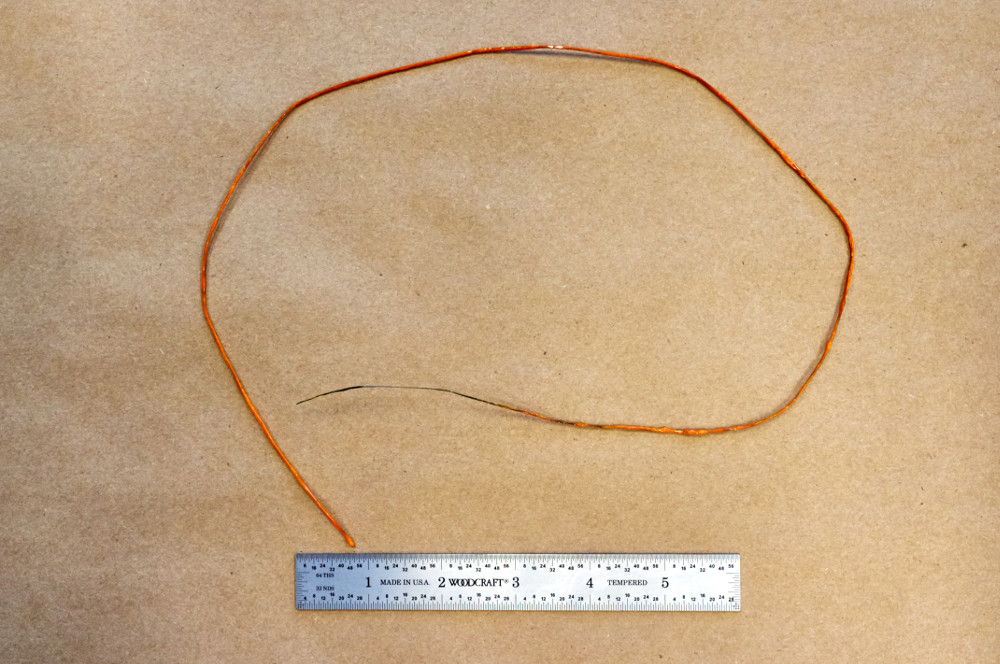
\includegraphics[width=0.8\textwidth]{./figures/filament-dipping-dried}
    \caption{A drying CFRP filament.}
    \label{fig:filament-dipping-dried}
\end{figure}



\begin{figure}[htp]
    \centering
    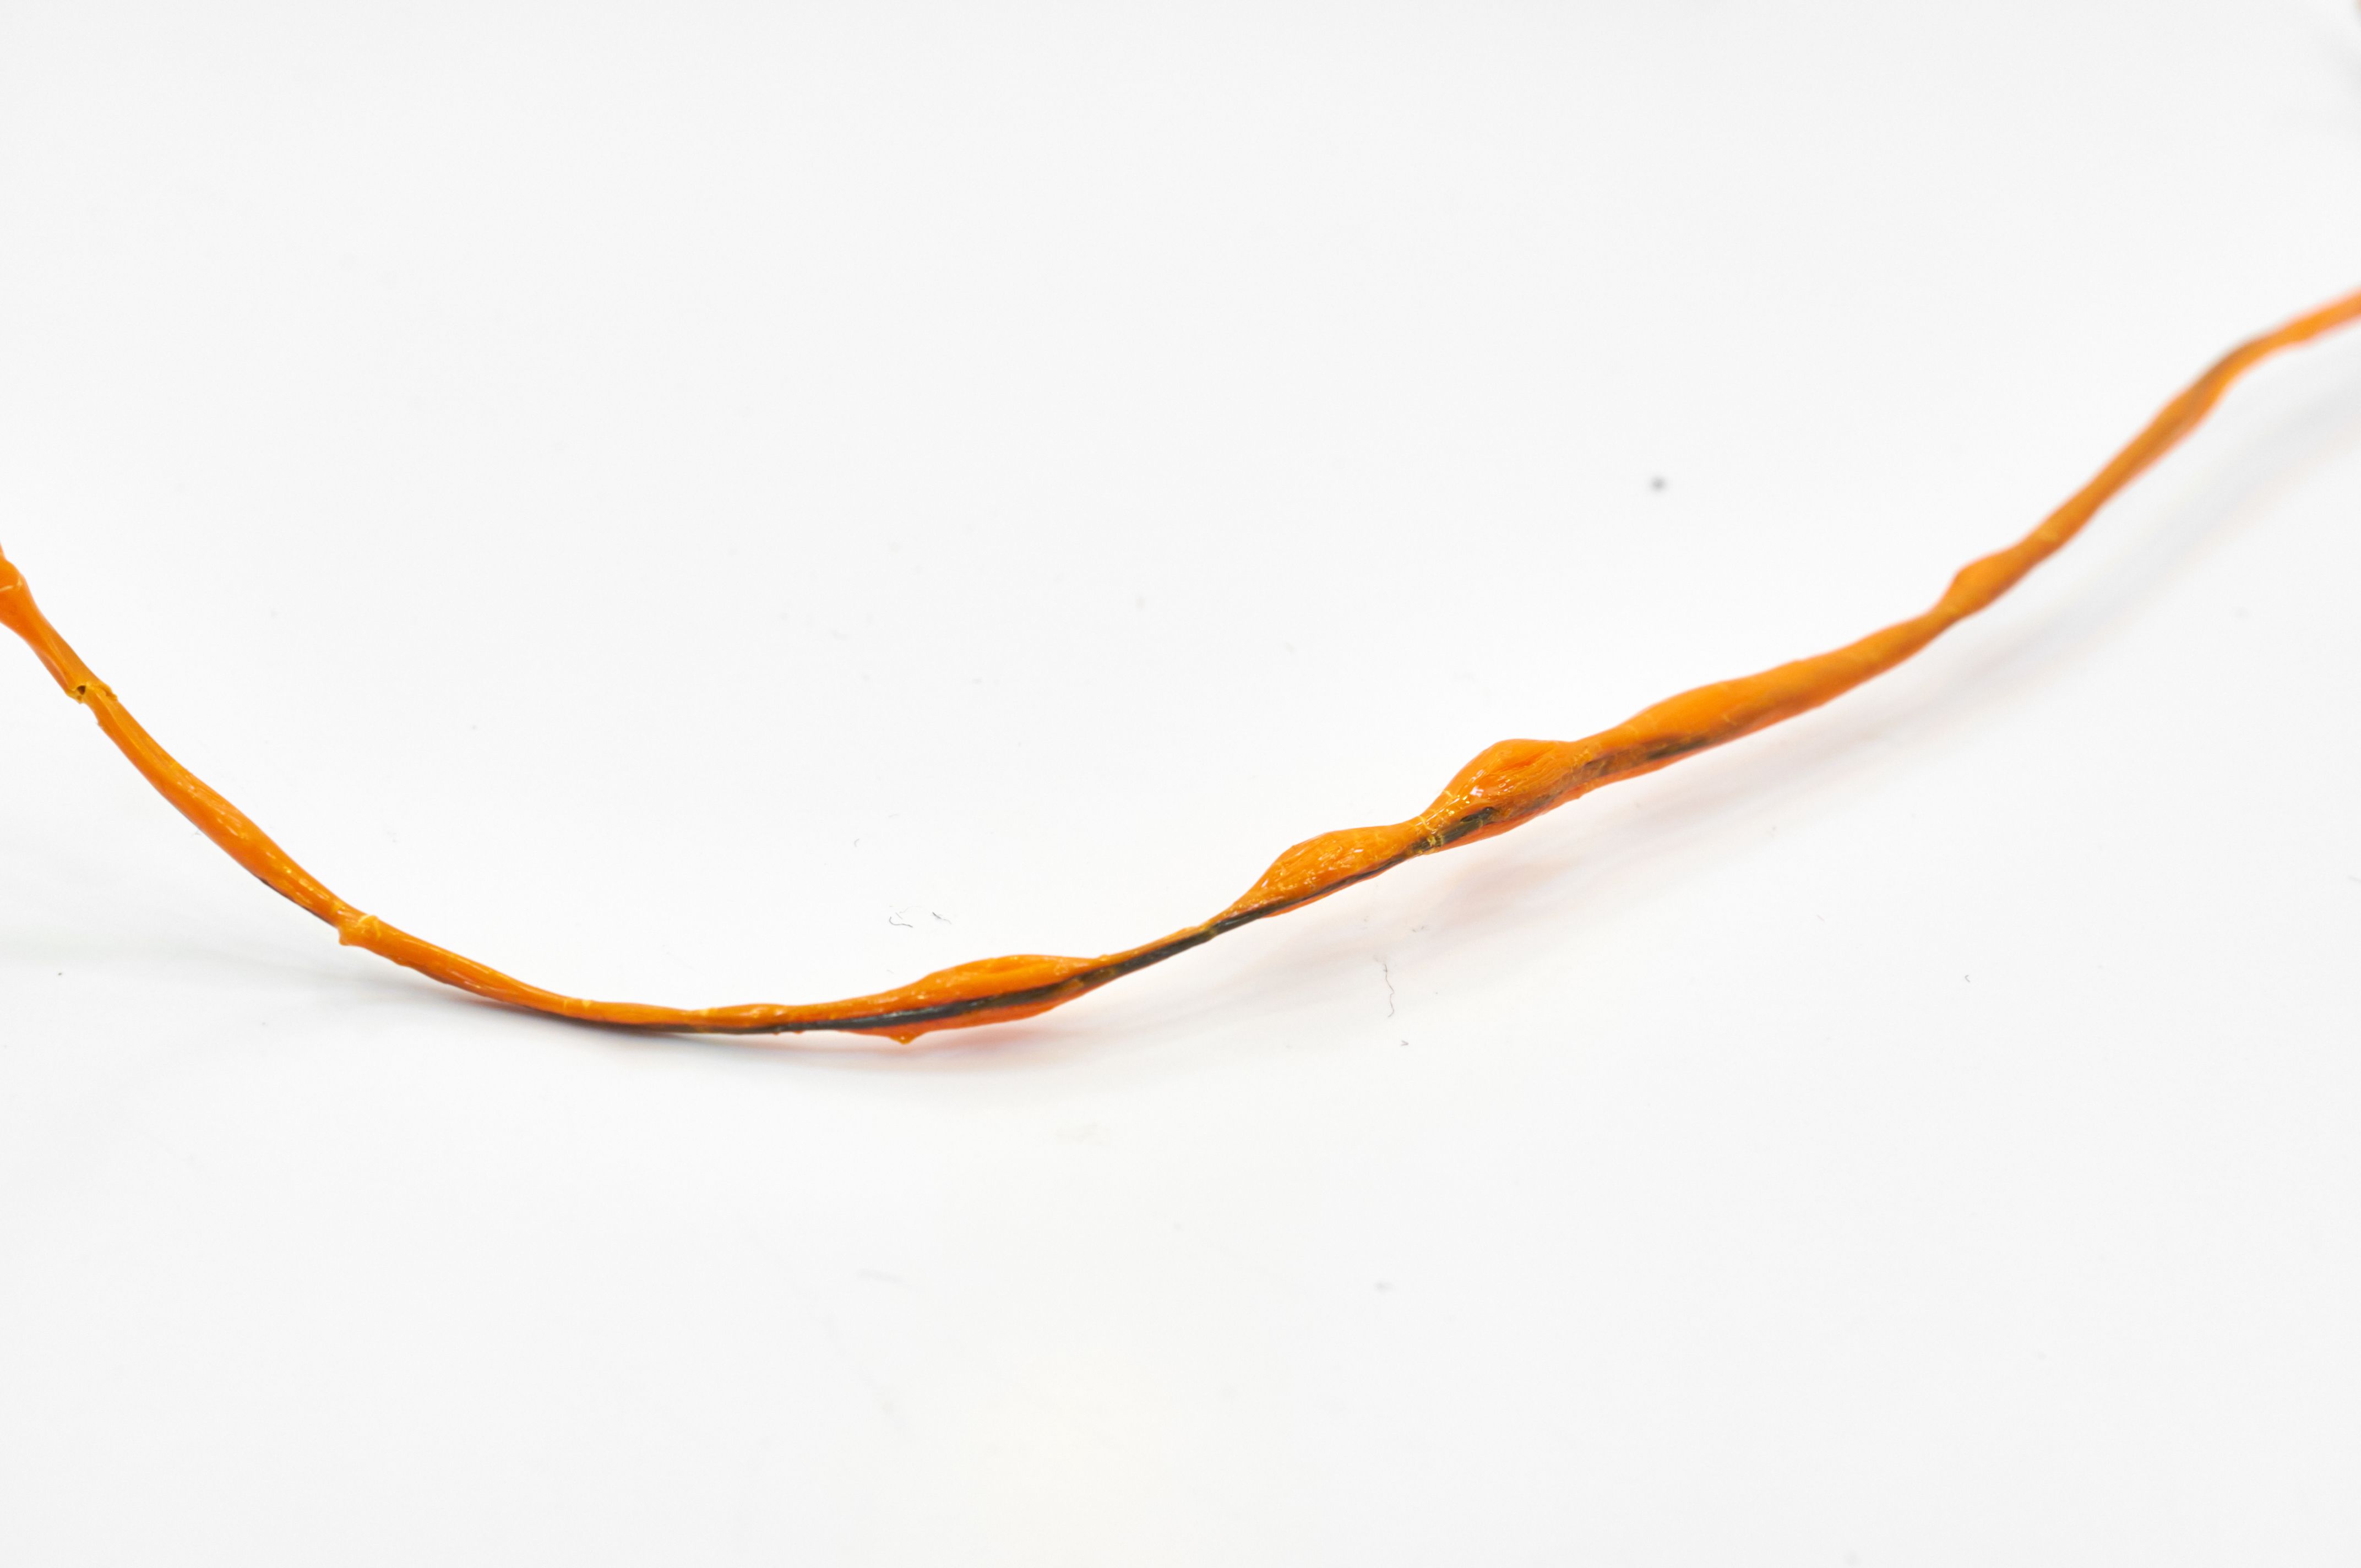
\includegraphics[width=0.8\textwidth]{./figures/filament-dipping-shear}
    \caption{CFRP filament with ABS sheared off from external guides.}
    \label{fig:filament-dipping-shear}
\end{figure}

\clearpage

\subsection{Mechanical Testing}

\indent

\subsubsection{Setup}

\indent

Tensile tests were performed on the filament samples that were produced using the pultrusion and dipping methods. An Instron mechanical testing machine was used for these tests. Short lengths of filament (roughly 2 in) were cut from larger samples for testing. Due to the small, slippery,  and flexible nature of the filament samples, the regular serrated jaw inserts of the Instron tensile test jaws could not be used alone to secure the samples. Instead of clamping the samples directly in the jaws, the samples were securely mounted to aperture cards using melted ABS. The ends of the card were folded over the filament. Once clamped in the serrated jaws, the cardboard protected the filament from the jaws and held it securely in place. The card also assisted in aligning the filament with the jaws. Once clamped, the exposed portion of the card was cut with scissors, and the test was started.\\

\begin{figure}[h!]
    \centering
    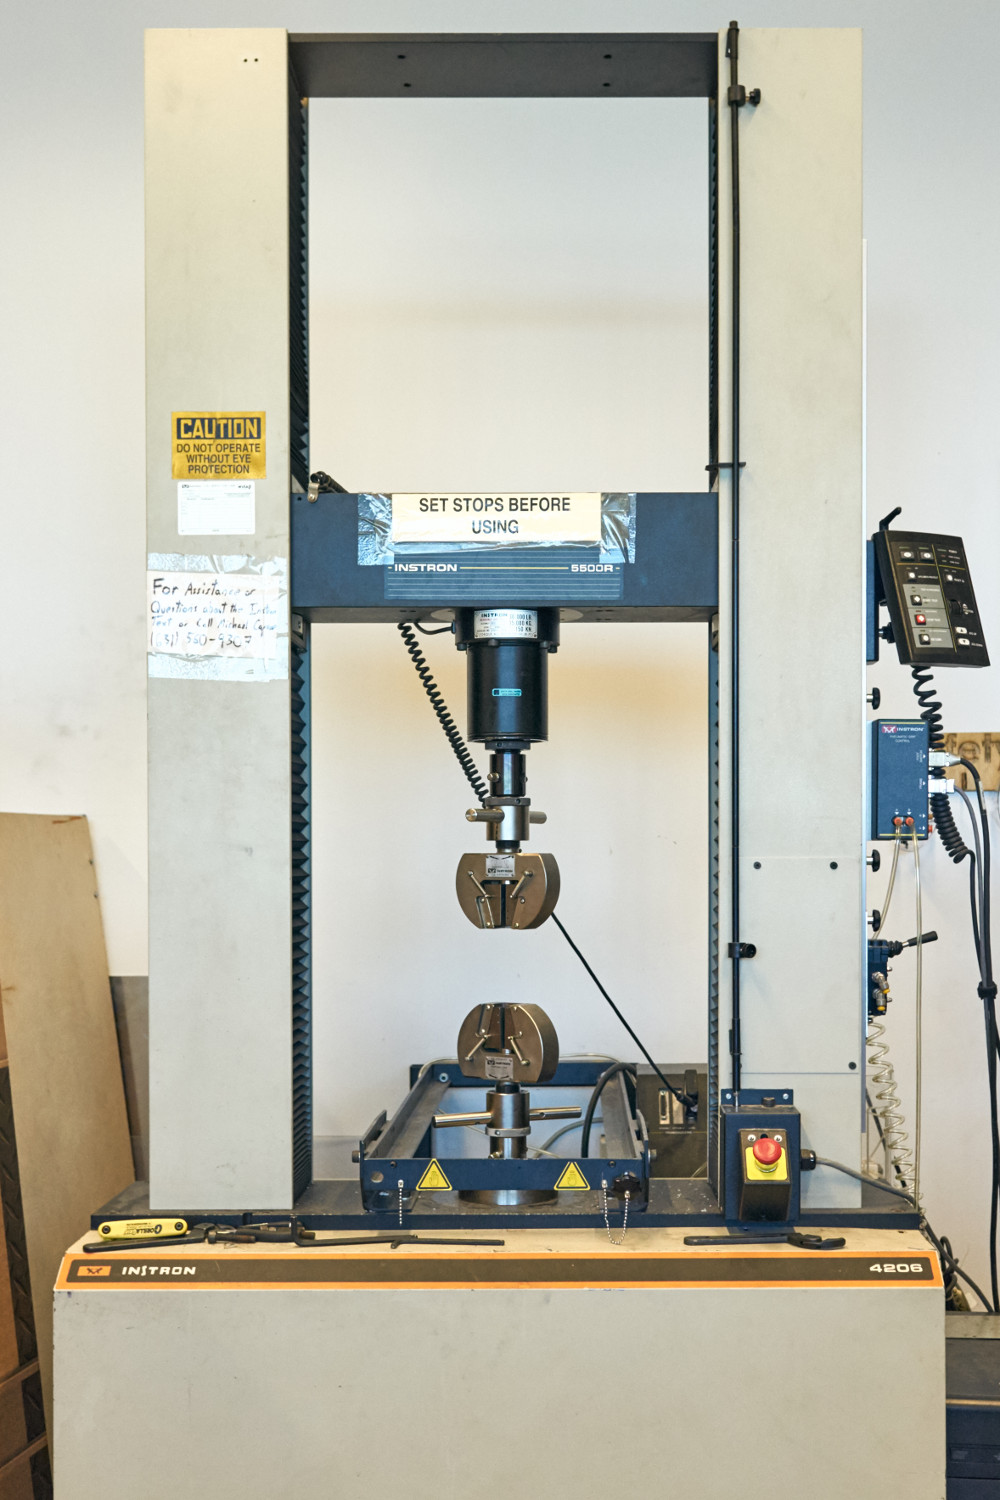
\includegraphics[width=0.5\textwidth]{./figures/intstron-overview}
    \caption{A photo of the Instron machine.}
    \label{fig:intstron-overview}
\end{figure}

\begin{figure}[h!]
        \centering
        \begin{subfigure}[b]{0.3\textwidth}
                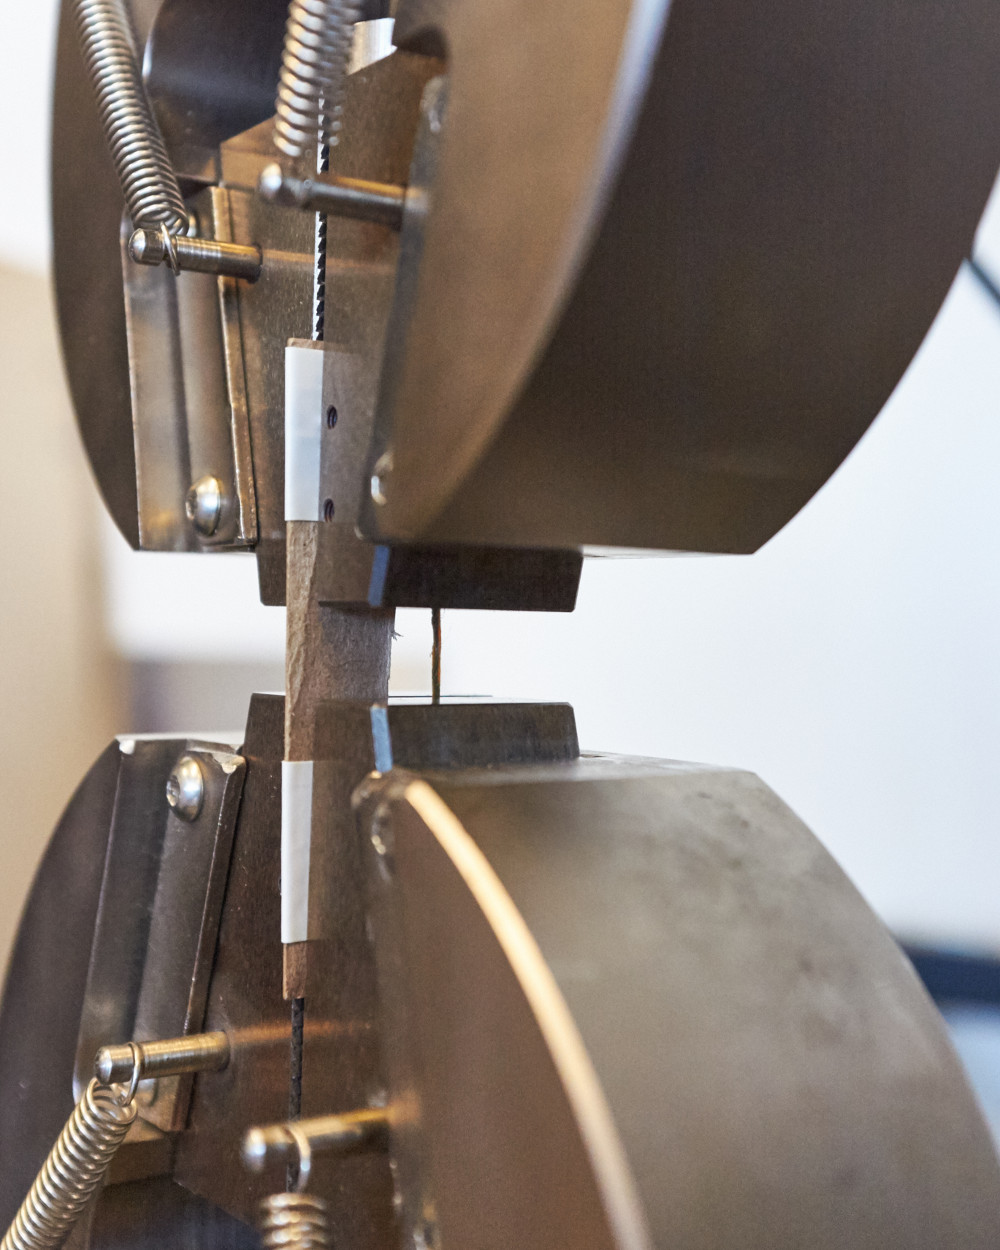
\includegraphics[width=\textwidth]{./figures/filament-instron-1}
                \caption{Installed in jaws.}
                \label{fig:filament-instron-1}
        \end{subfigure}
        \begin{subfigure}[b]{0.3\textwidth}
                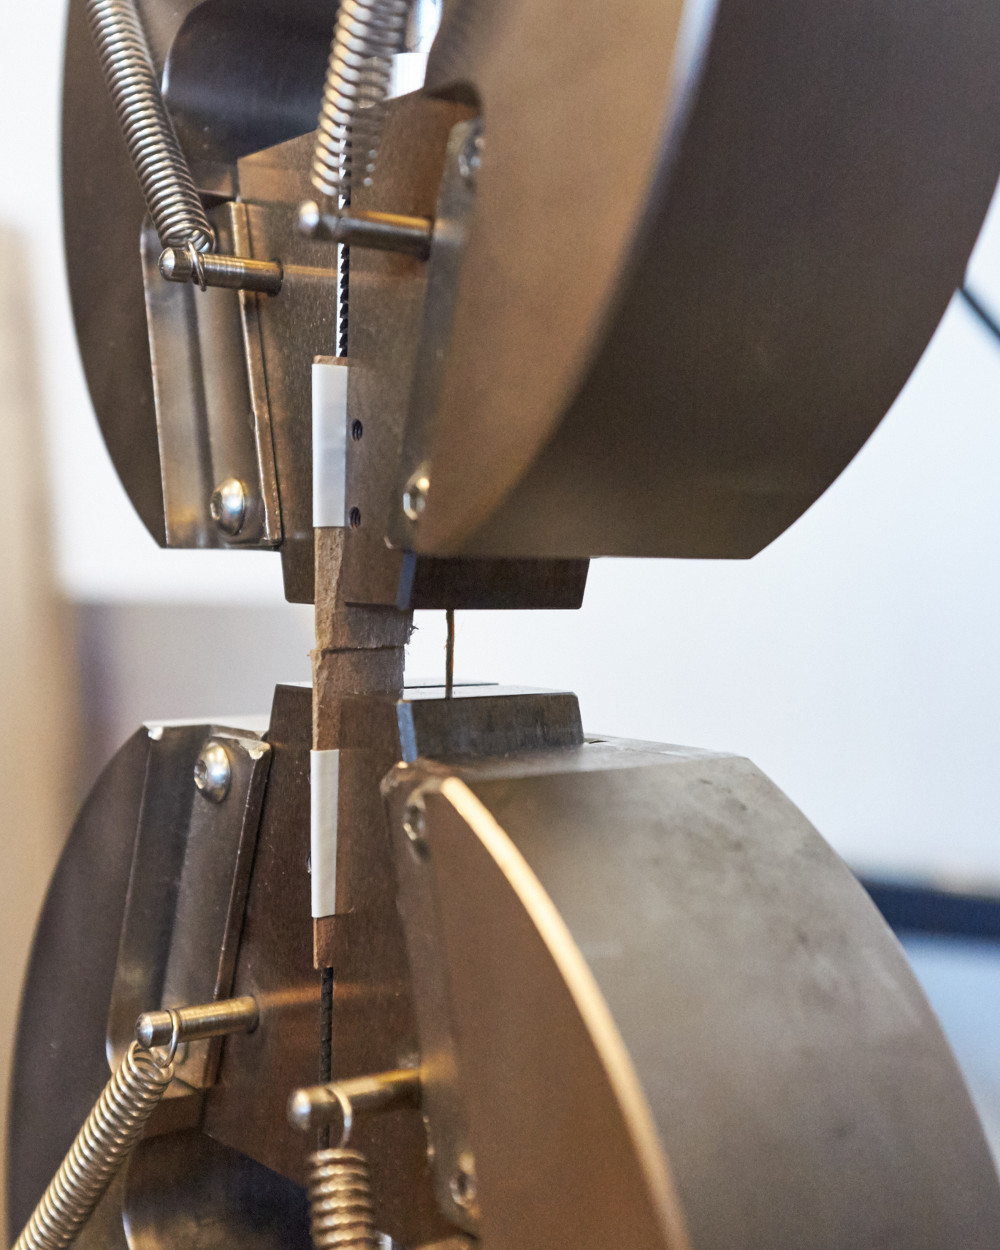
\includegraphics[width=\textwidth]{./figures/filament-instron-2}
                \caption{Cut card ready for testing.}
                \label{fig:filament-instron-2}
        \end{subfigure}
        \caption{A filament specimen loaded in the Instron for a tensile test.}
\end{figure}

\begin{figure}[h!]
    \centering
    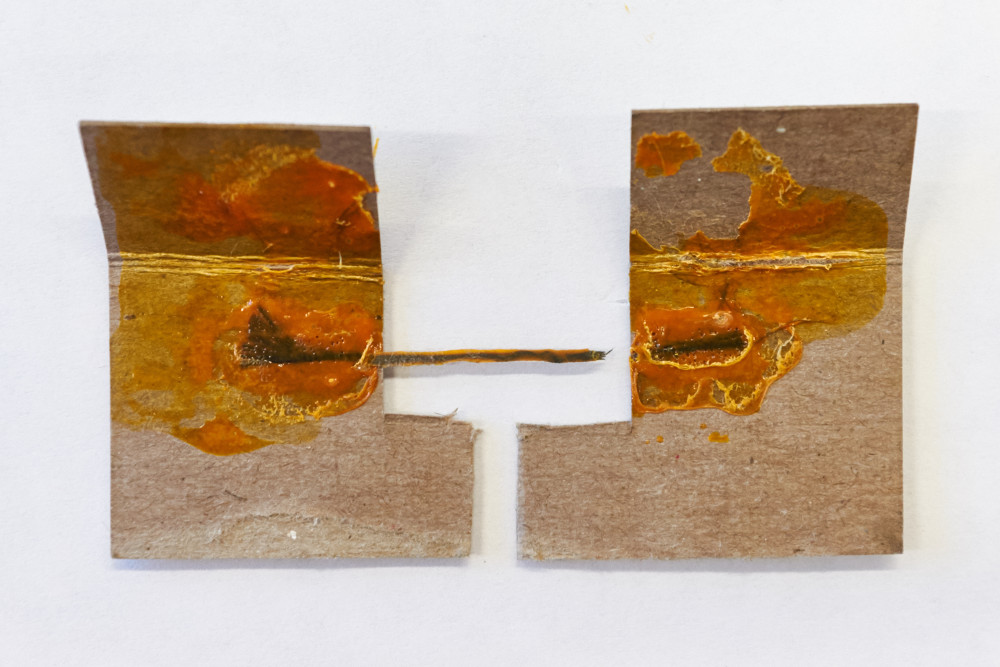
\includegraphics[width=0.5\textwidth]{./figures/filament-card-after-instron}
    \caption{A photo of a filament specimen after tensile testing.}
    \label{fig:filament-card-after-instron}
\end{figure}

\clearpage

\subsubsection{Results}

\indent

The tensile tests performed on the filament samples provide insight into some of their basic mechanical properties. A representative tensile test extension-load plot is provided in Figure~\ref{fig:instron-sample}. The CFRP samples showed fairly linear behavior before failing. Table~\ref{tab:test-results} compares the estimated ultimate tensile strength, stiffness, and density of two\footnote{Nearly a dozen samples were created. These two filaments selected for the table exhibited the most reasonable properties.} filament samples with those of ABS, carbon fiber, and aluminum 6061. The properties of aluminum were included for comparison because CFRP materials are often used to replace aluminum parts. Because it was difficult to consistently clamp the test samples without slipping once the test began, these are only very preliminary results. The results are also affected by inconsistencies in the filament samples themselves. Once the filament production method and test setup are further refined for consistency, further tests will be done to better characterize the properties of the filament. For now, however, the results are promising: both the pultruded and dipped filament samples are lighter and have a higher ultimate tensile strength than aluminum 6061, although they are not as stiff.\\

\begin{figure}[htp]
    \centering
    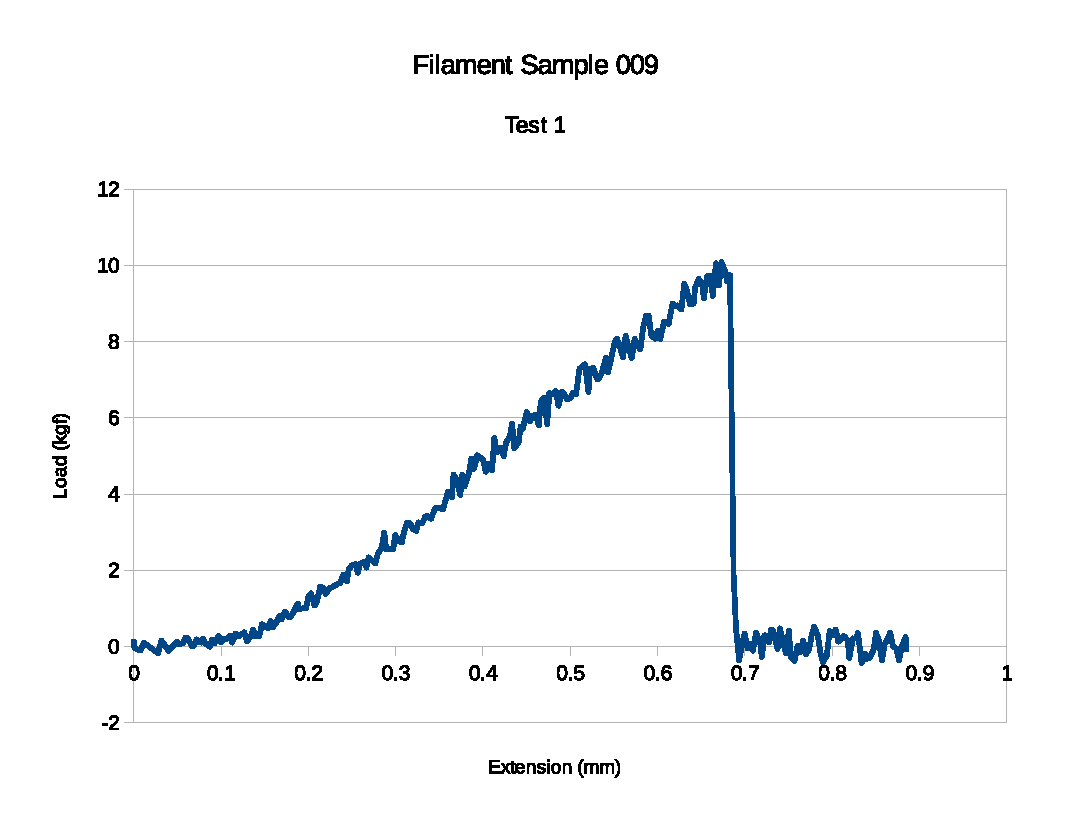
\includegraphics[width=0.8\textwidth]{./figures/009T1-instron-data}
    \caption{Sample tensile test data for a slurry-dipped filament sample.}
    \label{fig:instron-sample}
\end{figure}

\begin{table}[h]
    \centering
    \begin{tabular}{lcccc}
        Material           & Ultimate Tensile Strength (MPa)   & Stiffness (GPa)    & Density ($ kg/m^{3} $)  \\ \hline
        ABS                & 53                                & 2.3                & 1040 \\
        Carbon Fiber       & 3750                              & 231                & 1750 \\
        Aluminum 6061      & 310                               & 68.9               & 2700 \\
        Pultruded Filament & 313                               & 13.4               & 1354 \\ 
        Dipped Filament    & 690                               & 19.6               & 1567 \\
    \end{tabular}
    \caption{Preliminary CFRP filament test results, as compared to its constituents and to aluminum.}
    \label{tab:test-results}
\end{table}

\clearpage

\subsection{Print Testing}

\indent

\begin{figure}[h!]
        \centering
        \begin{subfigure}[b]{0.3\textwidth}
                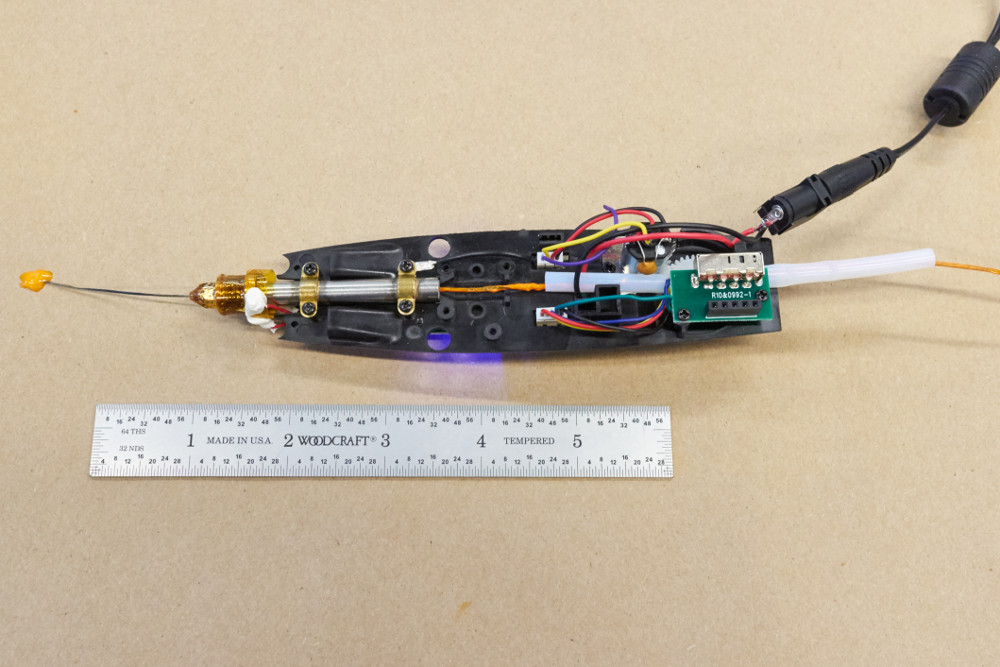
\includegraphics[width=\textwidth]{./figures/filament-print-3doodler-before}
                \caption{Before.}
                \label{fig:filament-print-3doodler-before}
        \end{subfigure}
        \begin{subfigure}[b]{0.3\textwidth}
                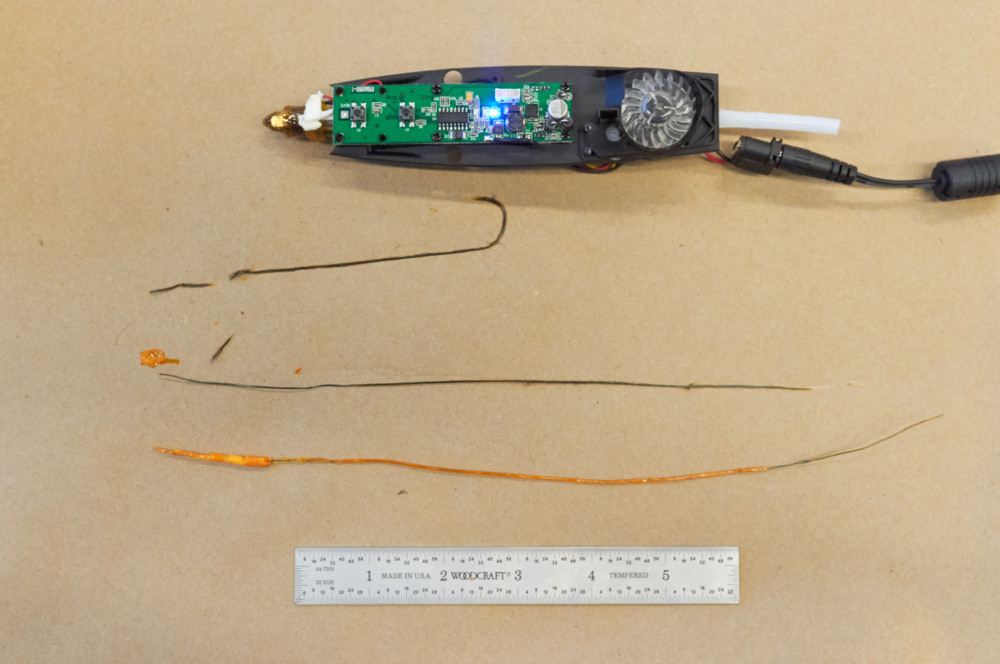
\includegraphics[width=\textwidth]{./figures/filament-print-3doodler-after}
                \caption{After.}
                \label{fig:filament-print-3doodler-after}
        \end{subfigure}
        \caption{Before and after shots of print testing with the CFRP filament.}\label{fig:filament-print-test}
\end{figure}

\begin{figure}[htp]
    \centering
    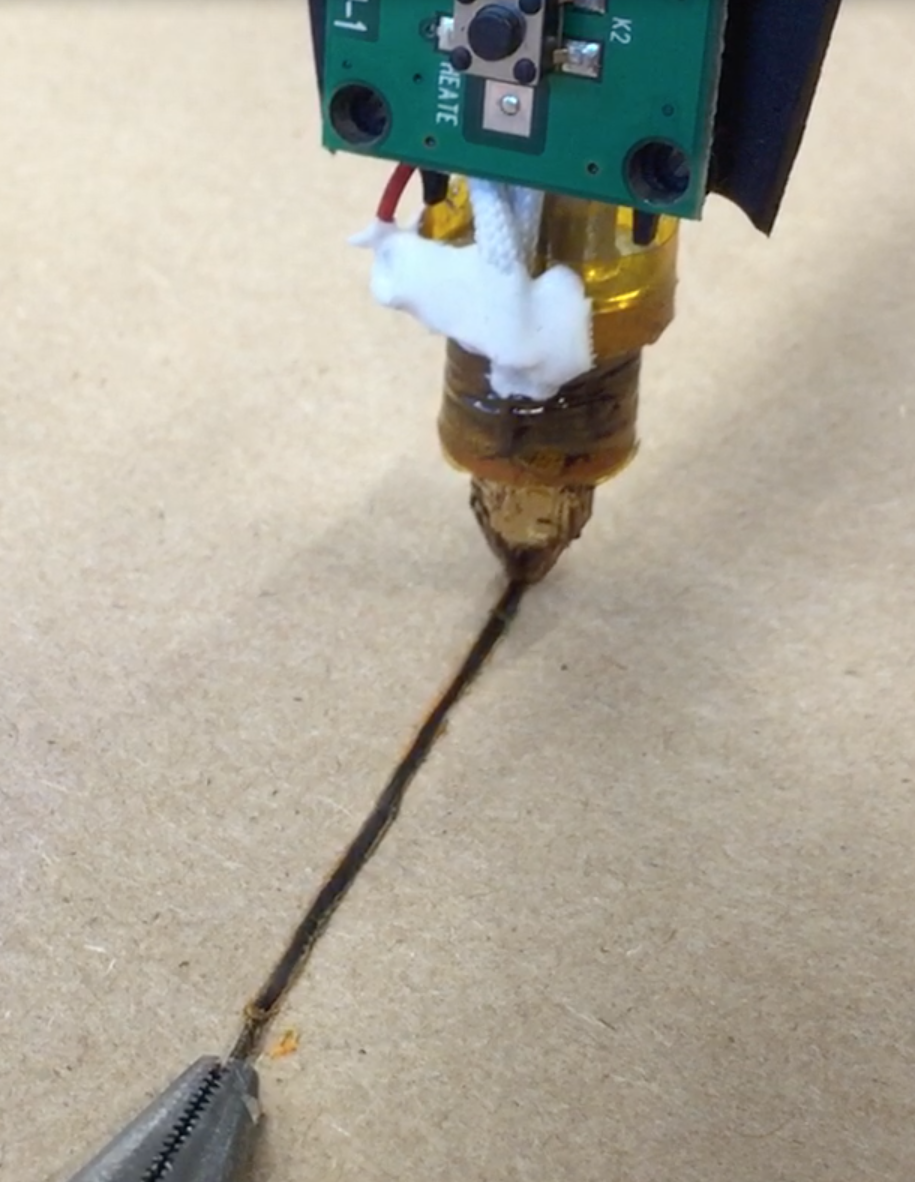
\includegraphics[width=0.5\textwidth]{./figures/filament-print-3doodler-during}
    \caption{Test printing the CFRP filament with a 3Doodler.}
    \label{fig:filament-print-3doodler-during}
\end{figure}

\begin{figure}[htp]
    \centering
    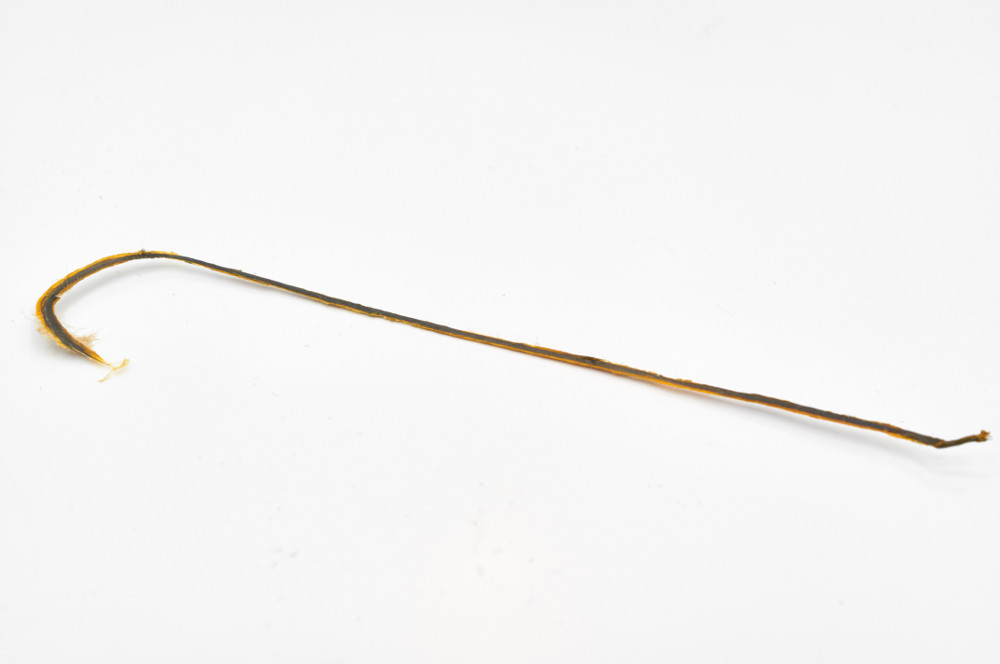
\includegraphics[width=0.8\textwidth]{./figures/filament-extrude}
    \caption{A close up photo of the filament printed with the 3Doodler}
    \label{fig:filament-extrude}
\end{figure}

\begin{table}[h]
    \centering
    \begin{tabular}{lcccc}
        Material           & Ultimate Tensile Strength (MPa)   & Stiffness (GPa)    & Failure Strain (\%)  \\ \hline
		Printed Filament & 338 & 7.63 & 4.44
    \end{tabular}
    \caption{Tensile test results for the printed CFRP filament}
    \label{tab:printed-filament-results}
\end{table}

\subsection{Future Suggestions}
%research and methods
\clearpage

%----------------------------------------------------------
%\section{Material Analysis}

\indent

Material analysis will be performed on the printed CFRP parts. Part geometry will be chosen such that CFRP curved layer, ABS curved layer, and ABS cartesian layer parts can be printed for comparison. Specific to part geometries, the Instron Tension Tester will be used to implement bending, compression and tensile tests as appropriate to quantify the strength and stiffness of each print. Strain gauges may even be placed along exposed fibers in attempt to determine fiber-specific stresses and strains.\\
% experimental stuff we haven't gotten to yet
\clearpage

%----------------------------------------------------------
\section{Finite Element Analysis}

\indent

Finite element analysis was used to predict the load-bearing capacity and failure behavior of the sample bridge specimen under the compressive load. The \textit{ANSYS Composite PrepPost} (ACP) package of \textit{ANSYS} finite element software was utilized due to suggestion of Cooper Union faculty\footnote{Professor Scott Bondi suggested that this software be used since he is familiar with package and could provided guidance.} and ease of access with Cooper Union's existing \textit{ANSYS} license. The following subsections primarily focus on FEA results and conclusions that can be drawn from the numerical analysis. However, rigorous explainations of the finite element models and physics models utilized in this study are located in \textit{Appendix: Composite FEA}.\\

\subsection{Finite Element Formulation}

\indent

ACP finite element modeling uses shell elements with orthotropic material properties to discretize geometry. The number of layers and thickness of each layer, which can be constant or variable, are given values. These parameters determine the overall thickness of each shell elemement, as well as the number of and spacing between integration points along the depth of each element. As such, the geometry input of ACP is a surface rather than a solid body. A reference direction is created within the model so that orthotropic element properties can be oriented accordingly with one direction representing the fiber, and other two being the matrix. In solving the model, Puck's failure criterion was used\footnote{The Tsai-Wu failure criterion was also considered due to its high frequency of appearance in research papers investigating carbon fiber 3D printing and curved layer 3D printing in general. However, Tsai-Wu failure was ultimately neglected since it required bi-axial stress data of the proposed filament, which could not easily be obtained.}. Puck failure is a phenomenological failure mode specifically suited for uni-direction (UD) CFRPs and glass fiber reinforced polymers (GFRPs) where inter-fiber failure\footnote{Failure of the matrix material, in shear, compression, or tension in a plane parallel to a plane contraining UD fibers.} (IFF) is most likely, which makes it the optimal failure mode for the FEA of the bridge specimen. Additionally, Puck Failure is intended for use with modeling inter-fiber failure (IFF) \large{\textbf{CITE}}. Table~\ref{fig:fea-bridge-speciment} shows the specific dimesions of the bridge geometry used in this analysis.\\

\begin{figure}[htp]
\centering
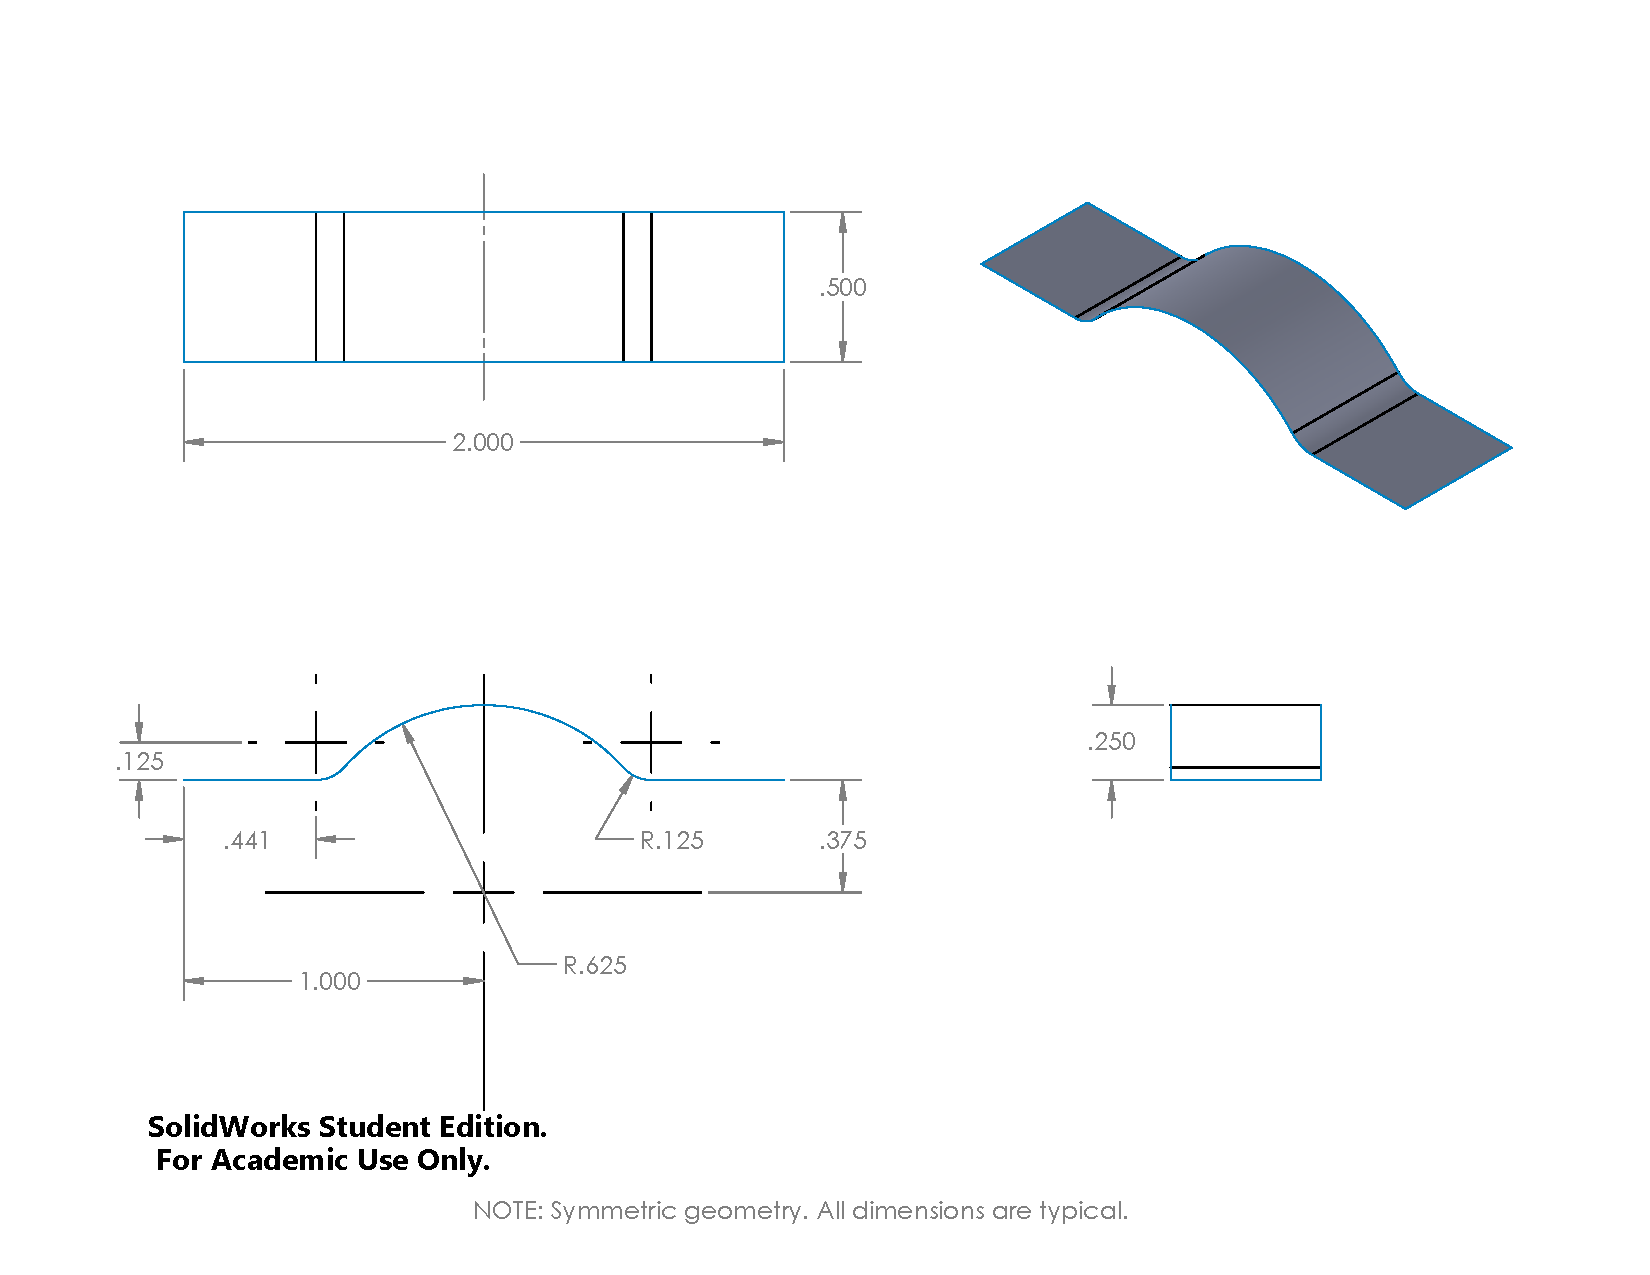
\includegraphics[width=1\textwidth]{./figures/fea/fea-surface-geometry}
\caption{The surface geometry used in ACP.}
\label{fig:fea-bridge-speciment}
\end{figure}

\clearpage

\subsection{ACP Results}

\indent

Figure~\ref{fig:fea-acp-tot-def} through Figure~\ref{fig:fea-acp-z-def} show the total and directional displacements of the loaded CFRP specimen loaded at 90 pounds-force, which puts the specimen just shy of failure. The units are in meters. Notable defection results are that the x-displacement of the loaded edge is on the same order of magnitude of the z-displacement of the central bend. Furthermore, the edges of the main bend warp slightly inward when the specimen is compressed (y-displacement).

%% Deformation

\begin{figure}[htp]
\centering
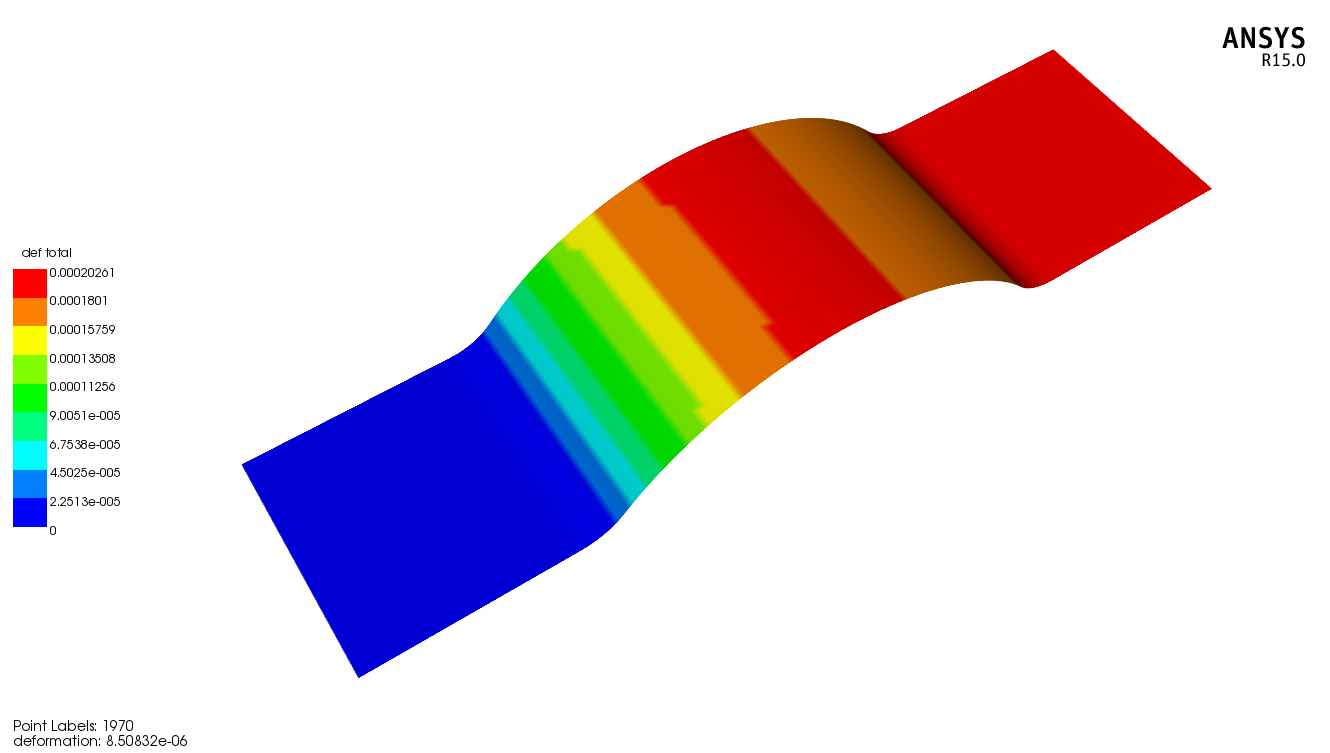
\includegraphics[width=1\textwidth]{./figures/fea/fea-acp-tot-def}
\caption{Total displacement FEA result.}
\label{fig:fea-acp-tot-def}
\end{figure}

\begin{figure}[htp]
\centering
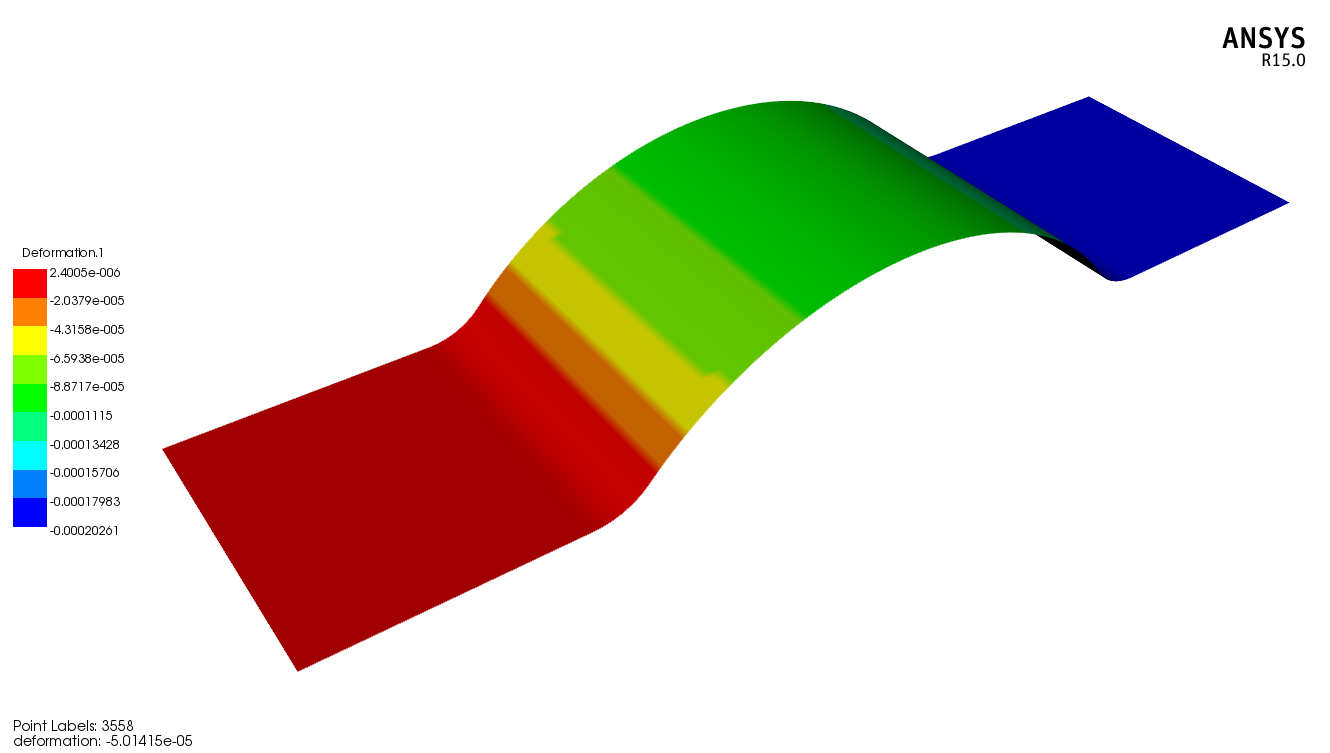
\includegraphics[width=1\textwidth]{./figures/fea/fea-acp-x-def}
\caption{X direction displacement FEA result.}
\label{fig:fea-acp-x-def}
\end{figure}

\begin{figure}[htp]
\centering
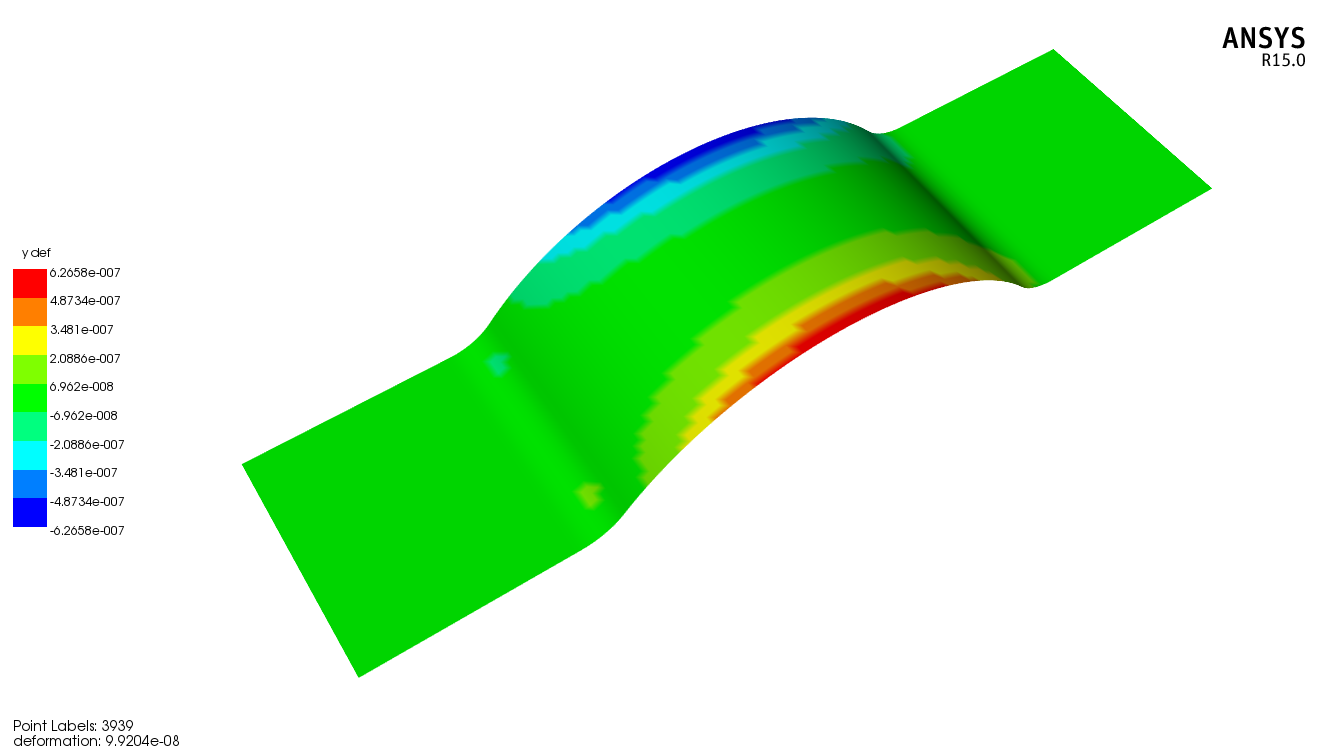
\includegraphics[width=1\textwidth]{./figures/fea/fea-acp-y-def}
\caption{Y direction displacement FEA result.}
\label{fig:fea-acp-y-def}
\end{figure}

\begin{figure}[htp]
\centering
\includegraphics[width=1\textwidth]{./figures/fea/fea-acp-z-def}
\caption{Mesh overview of the composite model in \textit{ACP} with a solid-body display state applied.}
\label{fig:fea-acp-z-def}
\end{figure}

\clearpage

%%% Puck Failure Results

Figure~\ref{fig:fea-acp-pfailure-notext} shows the resulting Puck failure. A value of 1 or above (red) indicates failure. While the two small fillets in the geometry see localized small spikes in value compared to their neighbors, the area of main concern is the central bend. Similar to the trends of typical mechanics of materials concepts, this section of the geometry experiences the largest bending moment of the entire body and is therefore most susceptible to failure. Figure~\ref{fig:fea-acp-pfailure-layer-closeup} shows a close-up of the critical portion of the geometry with the critical layer displayed above each element. Note that the bottom layer (ply 1) of the flat geometry and fillet is the failing layer. Just after the fillet, transitioning into the main curve, the middle layer (ply 30) is of main concern. Finally, the center of the specimen fails at the top layer (ply 60). Imploying concepts from bending in mechanics of materials, it is apparent that layers in bending tension are critical. Figure~\ref{fig:fea-acp-pfailure-mode-closeup} shows the same close-up but with failure mode information displayed on each element (\emph{pmC} denotes matrix shear failure, and \emph{pd} signifies delamination). Therefore, the mode of failure for this bridge specimen is matrix shear, which is then followed by delamination and additional matrix shearing. Note that near the boundaries of the part (the fixed edge and loaded edge), the specimen does not experience failure, it is mainly localized to the central arch.

\begin{figure}[htp]
\centering
\includegraphics[width=1\textwidth]{./figures/fea/fea-acp-pfailure-notext}
\caption{Puck Failure contour plot.}
\label{fig:fea-acp-pfailure-notext}
\end{figure}

\begin{figure}[htp]
\centering
\includegraphics[width=1\textwidth]{./figures/fea/fea-acp-pfailure-layer-closeup}
\caption{Closeup of Puck Failure contour plot with tabulated failing layer.}
\label{fig:fea-acp-pfailure-layer-closeup}
\end{figure}

\begin{figure}[htp]
\centering
\includegraphics[width=1\textwidth]{./figures/fea/fea-acp-pfailure-mode-closeup}
\caption{Closeup of Puck Failure contour plot with tabulated failure modes.}
\label{fig:fea-acp-pfailure-mode-closeup}
\end{figure}

\clearpage

\subsection{Comparison to Puck Failure Criterion}

\indent

Methods of composite failure are very specific to fiber and matrix material properties and the micromechanics of the structure. This makes a mathematical validation of FEA results nearly impossible with limited knowledge of the CFRP filament and 3D printed structure. However, qualitative trends from Puck's failure theory confirm the FEA findings.\\

Puck theorizes that $\theta_{fp} = 0^{\circ}$ transverse tension, $\theta_{fp} = 90^{\circ}$ through-thickness tension, $\theta_{fp} = 0^{\circ}$ positive inplane shear, $\theta_{fp} = 0^{\circ}$ negative inplane shear, $\theta_{fp} = 90^{\circ}$ positive transverse shear, $\theta_{fp} = 90^{\circ}$ negative transverse shear, $\theta_{fp} = +45^{\circ}$ positive through-thickness shear, and $\theta_{fp} = +45^{\circ}$ negative through-thickness shear are the fracture planes with the most significant impact on load bearing capacity of UD 3D geometry \large{\textbf{CITE}}. Logically then, the primary mode(s) of failure predicted for the bridge specimen should correlate to one or more of the previously mentioned IFF scenarios. Figure~\ref{fig:puck-failure-qualitative} shows the the loading of individual elements within the model which correlate to $\theta_{fp} = 90^{\circ}$ positive transverse shear (a) and $\theta_{fp} = 90^{\circ}$ through-thickness tension (b). Element \emph{a} shows a central bridge piece, which is in bending tension. The element adjacently left exerts a pulls mainly horizontally and slightly downward due to the curvature of the piece. Within the examined element, these forces are reacted to create a positive transverse shear load with a $90^{\circ}$ fracture plane (light grey) parallel to the fibers (dark grey). This same failure mode iis by the same reasoning evident in the portion of the fillet experiencing tension. Element \emph{b} depicts and element in the middle ply between two curves. Since elements to its upper right, and bottom left are are in tension, the examined element is bi-axially loaded. The large horizonatl load is reacted by the strong fibers while the matrix then experiences vertical tensions and completely separates in delamination, which is characteristic of the $\theta_{fp} = 90^{\circ}$ through-thickness tension failure mode. Therefore, qualitative analysis of the specimen using Puck's failure theory agree with finite element results.\\

\begin{figure}[htp]
\centering
\includegraphics[width=1\textwidth]{./figures/fea/puck-failure-qualitative}
\caption{Diagrams of Puck IFF in the bridge specimen.}
\label{fig:puck-failure-qualitative}
\end{figure}

\clearpage

\subsection{Comparison to Aluminum and ABS}

\indent

For comparison, standard solid-body finite element analyses were also performed with the materials properties of ABS and aluminum under the same 90 pound-force compressive load from the CFRP study. The setup of these finite element models, as well as contour plots of the results are located in \textit{Appendix: Composite FEA}. The factor of safety and the absolute values of directional deformations are located in \ref{tab:fea-cfrp-al-abs}. The factor of safety applied to the CFRP part is unity due to utilizing a load that puts the piece on the brink of failure. Following this convention, a positive factor of safety in another material denotes the margin that the load can be increased prior to reaching the ultimate tensile stress of the material. Similarly, a negative value indicates the margin by which the ultimate strength is surpassed by the applied load.

\begin{table}[htp]
    \centering
    \begin{tabular}{lcccc}
    
        Material & Factor of Safety & X Displacement, \emph{in} & Y Displacement, \emph{in} & Z Displacement, \emph{in} \\ \hline
        CFRP & 1 & 9.4E-05 & 2.5E-05 & 6.2E-03 \\
        Aluminum & 3.1 & 3.5E-05 & 5.9E-05 & 1.3E-05 \\
        ABS & 0.6 & N/A & N/A & N/A \\
                
    \end{tabular}
    \caption{Summary of CFRP, ABS, and aluminum FEA results.}
    \label{tab:fea-cfrp-al-abs}
\end{table}

The results show that a solid aluminum piece, which would likely be cast or machined to this shape, could withstand a load of 279 pounds-force prior to reaching its ultimate tensile strength of 42 \emph{ksi}. However, a part made purely of solid ABS would fail at a load of 54 pounds-force where it reaches its ultimate flexural stress of 8.5 \emph{ksi}\footnote{Plastics do not necessarily fail like typical ductile materials, such as aluminum, for which failure is assumed to occur when the ultimate tensile stress is reached. In the case of a plastic bending to failure, peak stress values are compared against the plastic's ultimate flexural stress}. Note that as a solid-body study, the ABS factor of safety is highly conservative as it negates the effects of voids and delamination\footnote{While many failure criteria within ACP are equipped to handle delamination and material degredation factors like voids, they are specific to composite failure modes. Subsequently modeling pure ABS in ACP would have yielded nonsensical results} that would be present in a 3D printed ABS part compared to an injection molded piece.\\

With regards to stiffness, the CFRP part exhibits deflection on nearly the same orders of magnitude as the aluminum piece. Given that carbon fiber is typically considered as a lightweight replacement for aluminum, this result is not surprising. Note that the ABS section of the table does not contain any deflection values. Due to the low stiffness properties of plastics, FEA analysis indicated that the structure would yield and impact itself in compression before actually reaching the 90 pounds-force of applied load. This phenomenon further suggests inflation in ABS's factor of saftey value in \ref{tab:fea-cfrp-al-abs}. While experimental data from physical compression tests using Cooper's Instron Tension Tester would more accurately depict the strength and stiffness properties, these finite element analyses suggest promising and statistically distinguishable trends.

\subsection{Discussion}

\indent

Overall, a finite element analysis of the CFRP bridge specimen using ACP and applying Puck's failure theory demonstrate the compressive load bearing capacity of this specimen to be 90 pounds-force. The finite element model was qualitatively validate with trends in the UD 3D interpretation of Puck's theory. These results predict a printed specimen that is nearly twice as strong as a pure ABS counterpart and is roughly as stiff as an aluminum analog. Going forward, experimental data will be necessary to accurately rate the strength of printed parts since all FEA models contain some error. Experimentation may also illuminate material roperty differences between the CFRP filament strands and extruded CFRP filament strands\footnote{Puck's failure theory contains degredation factors that account for defects such as voids and localized but frequently spaced ares of poor fiber wet-out, etc. ACP defaults to conservative standard degredation values so hopefully any of these slight differnces will have a neglible effect.}, which may need to be accounted for in future finite element analyses.

\clearpage


% fea section
\clearpage

%----------------------------------------------------------
\section{Print Controls}

\subsection{Approach}
There are many ways to create an FDM 3D printer, as seen in the many models available on the market, from industry-serving companies like Stratasys\footnote{\url{http://www.stratasys.com/}} and 3D Systems\footnote{\url{http://www.3dsystems.com/}} to home printer startups like Makerbot\footnote{\url{http://www.makerbot.com/}} to the many open-source efforts, notably the RepRap\footnote{\url{http://reprap.org/}} ecosystem. Most of these printers operate on Cartesian-style gantry system with 3 degrees of freedom. Some curved-layer printing is attainable on such printers, but the fixed attitude of the print heads limits the layer geometries to those that are accessible from one approach angle. To get around this limitation, a 6-degree-of-freedom robotic arm from FANUC\footnote{\url{http://www.fanucamerica.com/}} was used for this project. In addition to providing the 6 degrees of freedom necessary for curved-layer printing, the robot also provides 0.02mm of positioning repeatibility, which is small with respect to typical FDM nozzle outlet diameters (0.2-0.4mm). The robot was purchased in 2010 in the iRVision package as part of the CERT Program from FANUC. See the program brochure in Section~\ref{sec:cert-brochure} for more details.

Once the robot was chosen as the printing platform, much of the remaining 3D printing toolchain was filled in with parts and software from the RepRap community. These included the extruder hot-end and some related control hardware and software. Some additional control components were purchased from FANUC or fabricated in-house.

\subsection{Overview}
Figure~\ref{fig:sys-overview} gives a schematic overview of the mechanical, hardware, and software components that make up the curved-layer 3D printer system. The robot arm is the mechanical platform for the 3D printer. The custom extruder is fitted to the end of the robot arm and acts as a printing end effector. The motion of the robot arm is controlled by the robot controller, which is programmed by writing TP programs via the controller teach pendant. The extruder hardware, including the heater cartridge, cooling fan, and extrusion motor are controlled by an open-source Megatronics board loaded with the (also open-source) Marlin\footnote{\url{http://reprap.org/wiki/Marlin}} firmware. 

Normally, the Megatronics board is used to control the path of the extruder as well as the extrusion feed rate; the Marlin firmware can thus adjust the extruder filament feedrate according to the surface speed of the extruder in order to maintain the desired volumetric flow rate of hot plastic. However, in this case, the extruder path is controlled by the robot controller, so the extrusion control is independent of the motion control. Ideally, the two systems would be interfaced to allow the robot controller to give look-ahead speed predictions to the extruder controller to allow for tight synchronization. However, the FANUC controller interface only allows such interfacing with approved machinery. The next best option was to add I/O hardware to the FANUC controller and output an analog robot speed signal to the extruder controller. This way, the extruder controller might be able to extrude filament reasonably close to the actual extruder speed by tracking the robot speed output.

\begin{figure}
    \centering
    \includegraphics[width=.8\linewidth]{figures/diagrams/system overview}
    \caption{Overview of the 3D printer controls.}
    \label{fig:sys-overview}
\end{figure}

A more detailed electrical schematic is shown in Figure~\ref{fig:schem-fig}. 

\begin{figure}
    \centering
    \includegraphics[width=.8\linewidth]{figures/diagrams/schematic-figure}
    \caption{Electrical schematic of the 3D printer controls.}
    \label{fig:schem-fig}
\end{figure}


\subsection{FANUC I/O interface}
The FANUC robot controller makes digital and analog electrical signals available to the user through the teach pendant interface \cite[sec~3.1.3]{lr-handling-tool}. However, in order to physically access these signals, additional I/O hardware is required. For this purpose, a FANUC backplane was purchased, as well as a corresponding I/O interface model and analog output module. Installation, maintenance, and usage information for these parts is available in \cite{io-unit}. The backplane and I/O interface module were purchased together as part of an I/O starter kit\footnote{from an eBay surplus seller.} for R-30iA controllers. The kit also included the I/O link cable, which connects the I/O interface unit to the controller and optional additional interface units; a grounding wire assembly for the backplane; and a male-male wire assembly for powering the I/O interface module. The analog output module was purchased separately. 

\subsubsection{Modules}
The I/O Unit Model A (interface module) makes the I/O points of the FANUC robot controller accessible through additional I/O modules. The interface module is installed in the first slot of the backplane, as shown in \cite[p~10]{io-unit}. The analog output module is installed in the next slot, and the remaining four slots are left empty.

\subsubsection{Wiring and connections}
The I/O interface module is connected to the controller and power supply according to \cite[ch~4]{io-unit}. In some configurations, the I/O interface unit would receive power from an auxiliary controller (a CNC machine, for instance) over the included cable. In this case, an external supply was needed. Additionally, the included grounding wire was too short to reach the inside of the existing FANUC controller from its desired location on the backplane. Thus, a power supply (CUI Inc EPS240025-P5P, datasheet in Section~\ref{sec:io-power}) and grounding wire were selected according to \cite[sec~4.2]{io-unit} and \cite[sec~4.3]{io-unit}, respectively. The power supply was spliced to the included power wire; the result is shown in Figure~\ref{fig:io-power}. Figures~\ref{fig:io-door} and \ref{fig:io-ground} show the I/O link cable connected on the back of the controller door and attached to the grounding plate as shown in \cite[Fig.3.2.2]{controller-maintenance}. Figure~\ref{fig:io-ground} also shows the installed ground wire for the I/O backplane, as described in \cite[sec~4.3]{io-unit}.

The analog output module offers two channels, each with a voltage output and a current output. The Channel 0 voltage output was chosen; the module pinout is available in \cite[sec~7.1.3]{io-unit}.

\begin{figure}
    \centering
    \includegraphics[width=.8\linewidth]{figures/io-power-splice}
    \caption{I/O interface module power supply.}
    \label{fig:io-power}
\end{figure}

\begin{figure}
    \centering
    \includegraphics[width=.5\linewidth]{figures/diagrams/io-door-circled}
    \caption{I/O link cable installed in cabinet door.}
    \label{fig:io-door}
\end{figure}

\begin{figure}
    \centering
    \includegraphics[width=.8\linewidth]{figures/diagrams/io-ground-circled}
    \caption{I/O link cable and back plane grounding.}
    \label{fig:io-ground}
\end{figure}

\subsubsection{Housing design}
A housing cabinet was designed and built to protect the I/O modules and allow access for maintenance and further expansion. The installed cabinet is shown in Figures~\ref{fig:cabinet1} and ~\ref{fig:cabinet2}. The cabinet was designed with inside dimensions according to \cite[sec~3.2]{io-unit}. Because the total heat generation of the two modules is only 4.3W, according to \cite[Table~3.3]{io-unit}, no special ventilation features were added. Clear polycarbonate was chosen as the cabinet material for easy visual checking of the I/O interface module status lights and proper wiring. The polycarbonate panels were adhered together with a SCIGRIP acrylic cement\footnote{\url{http://www.scigrip.com/product.php?id=16}}. The cabinet mounts to the CERT cart frame alongside the FANUC controller. Felt washers, shown in Figure~\ref{fig:felt-washer}, were used to protect the cabinet bottom from the frame members. Drawings and a bill of materials for the cabinet are available in Appendix~\ref{sec:cabinet-drawings}.

\begin{figure}
    \centering
    \includegraphics[width=.5\linewidth]{figures/cabinet1}
    \caption{The I/O cabinet.}
    \label{fig:cabinet-1}
    \end{figure}

\begin{figure}
    \centering
    \includegraphics[width=.8\linewidth]{figures/cabinet2}
    \caption{The I/O cabinet installed alongside the FANUC controller.}
    \label{fig:cabinet-2}
\end{figure}

\begin{figure}
    \centering
    \includegraphics[width=.8\linewidth]{figures/felt-washer}
    \caption{A felt washer in the I/O cabinet mount.}
    \label{fig:felt-washer}
\end{figure}

\subsection{Megatronics board}
The Megatronics\footnote{\url{http://reprap.org/wiki/Megatronics_2.0}} board is a microcontroller board designed to drive RepRap open-source 3D printers. The board itself is based on other open-source projects, namely the Arduino Mega 2560\footnote{\url{http://www.arduino.cc/en/Main/arduinoBoardMega2560}} and the RAMPS\footnote{\url{http://reprap.org/wiki/RAMPS}} electronics design. The core features of the board are the ATmega 2560\footnote{\url{http://www.atmel.com/devices/atmega2560.aspx}} microcontroller, the Pololu stepper driver\footnote{\url{https://www.pololu.com/category/120/stepper-motor-drivers}} slots, and the extruder signal pins. The board is also set up for optional dual extruders, a heated bed, and an LCD display among other additional features. The Megatronics board was chosen for this project mostly out of convenience: although few of the board's features are used here, its compatibility with exsisting firmwares and control modules made the setup relatively easy compared to making a custom pared-down controller board. A datasheet for the board is available in Appendix~\ref{sec:mega-datasheet}.

\subsubsection{Mounting}
The Megatronics board is mounted to the frame of the CERT robot cart such that the board is accessible for modifications and the wires reach the extruder readily. The mount location also facilitates USB connection to a laptop for uploading new firmware\footnote{A 16ft USB cable was initially used in hopes of routing the cable through the frame for easy access in case the board was moved to a less accessible location. The resulting avrdude sync errors prevented any programs from uploading properly even though the cable was shorter than the recommended 5m maximum. Using a 2ft cable alleviated the problem.}. The mounted board is shown in Figure~\ref{fig:mounted-mega}. Drawings and a bill of materials for the mount are available in Appendix~\ref{sec:mega-drawings}.

\begin{figure}
    \centering
    \includegraphics[width=.8\linewidth]{figures/mounted-mega}
    \caption{The mounted Megatronics board.}
    \label{fig:mounted-mega}
\end{figure}

\subsubsection{Wiring and connections}
In order to keep the wires neat where they met the board, the acrylic mount was designed with cable-tie slots, and the extruder wires were bundled in expandable polyester sleeving. These are shown in Figure~\ref{fig:mega-back}. The power and analog input wires to the board both terminate somewhere in the bottom portion of the cart, so those wires were routed through the slots in the cart's auminum extrusions, shown in Figure~\ref{fig:frame-wire-route}.

\begin{figure}
    \centering
    \includegraphics[width=.5\linewidth]{figures/megatronics-back}
    \caption{Wire managament at the Megatronics board.}
    \label{fig:mega-back}
\end{figure}

\begin{figure}
    \centering
    \includegraphics[width=.8\linewidth]{figures/frame-wire-route}
    \caption{Wires routed through the cart frame slots.}
    \label{fig:frame-wire-route}
\end{figure}

\subsubsection{Firmware}
The Megatronics board is compatible with the Marlin open-source 3D printer firmware. The board is generally supplied with the Marlin firmware already uploaded, but the board is open to modified or completely different firmwares in case of other development projects. The Marlin firmware exists as a Git repository hosted on Github\footnote{\url{https://github.com/}}. See Appendix~\ref{sec:more-info} for more information on Git.

Before attempting to use the full Marlin firmware, the board was tested for basic functionality using the supplied test firmware\footnote{\url{http://reprap.org/wiki/Megatronics_2.0\#Files}}. Once the board functionality was confirmed, the Marlin firmware was forked\footnote{\url{https://help.github.com/articles/fork-a-repo/}} and configured\footnote{\url{http://reprap.org/wiki/Marlin\#Configuring_and_compilation}} for this project's custom extruder. The new repository is linked in Appendix~\ref{sec:more-info}. Note in \verb|Configuration.h| that the extruder \verb|e_steps_per_mm| is calculated from on the stepper motor, gear ratio, and effective filament drive diameter of the custom extruder. Also note that \verb|FAN_PIN| and \verb|FAN2_PIN| are swapped because the Megatronics board is (for reasons unknown) missing screws from the screw terminals for Fan 1.

\subsubsection{Software}
Once the Megatronics board is set up, it is ready to take commands from a computer. It accepts G-code\footnote{\url{http://en.wikipedia.org/wiki/G-code}}, in this case, over a USB interface. G-code for RepRap 3D printers usually includes extruder motion commands, speed settings, heater temperature settings, fan speeds, and more. Usually, a 3D printed part starts as a 3D model file such as an \verb|.stl| or a \verb|.step|. A piece of computer software "slices" the model, creating the toolpath necessary to print the file. The software also uses information about the 3D printer's geometry and printing hardware to generate the appropriate G-code. Later, the computer sends the G-code to the 3D printer controller, the Megatronics board in this case, which then interprets the G-code and creates the printed part.

For this project, there is not yet any software that handles curved-layer FDM 3D printing. Thus, the "slicer" portion of the software will not be used yet. Because the extruder motion control is all handled by the FANUC robot, for now, all that is needed is a G-code sending application to control the extruder heating, cooling, and feed. Pronterface, part of the Printrun\footnote{\url{http://reprap.org/wiki/Printrun}} package, was chosen to send G-code to the Megagronics board. Pronterface is a GUI (graphical user interface) that simplifies interfacing with RepRap printers, especially while debugging the extruder itself. 

The main Pronterface interface is shown in Figure~\ref{fig:pronterface}. At a glance, the interface allows the user to connect and disconnect from printers, change feedrates, jog the motors, and set heater setpoints in addition to providing a G-code command line.

\begin{figure}
    \centering
    \includegraphics[width=.9\linewidth]{figures/pronterface}
    \caption{The main Pronterface interface.}
    \label{fig:pronterface}
\end{figure}

\subsection{Jameco power supply}
\subsubsection{Current requirement}
The Megatronics board can be powered from a 5V USB connection or from a 12V external power supply, as determined by on-board jumpers (see the datasheet, Appendix~\ref{sec:mega-datasheet}). The USB power from a typical laptop is adequate for communicating with and programming the board. However, driving stepper motors and heating cartridges requires far more current than a laptop USB port can supply, so a Jameco OEM power supply was chosen to power the board. The supply is rated for 11.5A at 12V. The extruder stepper motor is rated at 1.7A/phase with two phases for a total current draw of \(1.7\si{\ampere}\sqrt{2}=2.4\si{\ampere}\). The ceramic heater is rated for 30W at 12V\footnote{\url{http://www.makerfarm.com/index.php/hexagon-hot-end.html}}, for a current draw of \(\frac{30\si{\watt}}{12\si{\volt}}=2.5\si{\ampere}\). There are no other significant electrical loads in the extruder, so the Jameco power supply is adequate for the custom extruder. The power supply datasheet is available in Appendix~\ref{sec:jameco-datasheet}.

\subsubsection{Mounting}
The power supply was mounted at the rear of the underside of the CERT cart bed frame. The mounted supply is pictured in Figure~\ref{fig:jameco-mounted}. The mounting location was chosen for easy access for future wiring activities. A clear acrylic cover was made to protect any person or foreign object from accidentally touching the screw terminals. The cover was laser cut and then bent to shape using a purpose-built strip heater, shown in Figure~\ref{fig:strip-heat}. Drawings and a bill of materials for the mounting setup are available in Appendix~\ref{sec:jameco-drawings}.

\begin{figure}
    \centering
    \includegraphics[width=.8\linewidth]{figures/jameco-mounted}
    \caption{The mounted Jameco power supply.}
    \label{fig:jameco-mounted}
\end{figure}

\begin{figure}
    \centering
    \includegraphics[width=.8\linewidth]{figures/strip-heat}
    \caption{Power supply screw terminal cover on the strip heater.}
    \label{fig:strip-heat}
\end{figure}

\clearpage

%----------------------------------------------------------
\section{Extruder}

An extruder end-effector was designed and fabricated for the carbon fiber 3D printer. The extruder is the mechanism responsible for depositing the filament in a 3D printing system. Generally, this mechanism includes a motor that drives a gripping mechanism, which reels in and pushes the filament into a nozzle. A heating element just prior the the nozzle melts the outside of the plastic filament while softening the interior. The molten filament is extruded through the nozzle outlet onto the printing bed or an already existing printed layer where it cools to create the part.\\

In the case of the curved layer carbon fiber 3D printer, the extruder was required to mount to the FANUC robot arm, be compact\footnote{The compact size is required for two reasons. First, to ensure that induced torque on the robot arm joints and gripper remain within safe operating conditions. Second, to readily permit the nozzle to deposit material when not perpendicular to the build platform, which will be required for printing curved layers.}, and accept filaments of a variety of sizes (likely ranging in diameter from 1.75 mm to 3 mm). \\

\subsection{Design}

\indent

Figure~\ref{fig:old extruder} presents the initial design of the extruder in \emph{SolidWorks}. This iteration of the extruder design mounted to the Fanuc grippers and was intended to be made from custom-machined components (acrylic and aluminum) and RepRap hardware (nozzle, J-head, J-head mounting plate, ceramic heating element, thermistor, fan, and fan mount). This configuration locates the nozzle outlet along the mid-plane of the grippers for simple coordinate transformations when programming the robot to print. Laser-cut acrylic gears provide a 3:1 step up in torque from the stepper motor and drive a notched screw, which grips and pushes the filament into the nozzle. A bearing opposite the screw provides counter-pressure and its mounting plates can adjust the distance between the screw and bearing to accommodate different filament sizes.\\

\begin{figure}[h!]
\centering
\includegraphics[width=0.5\textwidth]{./figures/extruder-old-2}
\caption{An isometric view of the initial extruder design.}
\label{fig:old extruder}
\end{figure}

To assess the feasibility of the initial extruder design, minor tweaks were implemented within the CAD to make a laser-cut prototype.  Figure~\ref{fig:prototype extruder} shows the prototype mounted on the FANUC grippers. The prototype served its purpose and demonstrated numerous problems with the initial design. There were some mis-measurements of RepRap hardware, using spacers instead of threaded standoffs decreased the rigidity of the structure, the structure was a bit larger than desired, and a few undetected interferences were discovered. Subsequently, the extruder went through a redesign phase to develop an acceptable configuration.\\

\begin{figure}[h!]
\centering
\includegraphics[width=0.5\textwidth]{./figures/extruder-prototype-2}
\caption{A photograph of the mounted prototype.}
\label{fig:prototype extruder}
\end{figure}

Figure~\ref{fig:extruder iso} presents a rendering of the final extruder design. Figure~\ref{fig:extruder drawing} provides general dimensions and annotations to fully present the extruder design concept. The final design was significantly smaller than the initial design, requird less machining, and used less fastening hardware. The size decrease was accomplished by using smaller gears (50\% scaled versions of gears dimensions taken from \emph{SDP-SI}\footnote{\url{http://www.sdp-si.com/}} and located the stepper motor directly beneath the FANUC grippers. As part of the design process the gears were laser-cut, and physically tested to ensure that the teeth would not shear off under a load less than the stall torque of the stepper motor, before being fully committed to this design. The stepper motor (Sparkfun ROB-10846) outputs 68 oz-in of torque and has a resolution of 400 steps/revolution. Two laser-cut acrylic gears step up the torque to 204 oz-in.\footnote{Most extruders in the 3D printing community use analogous stepper motors and utilize gear trains to step up the torque. Common gear ratios range from 2:1 to 4:1 depending on the specific qualities of the filament. Given that the specifics of the filament are not yet fully determined, the mean value was used.} In this design, a partially threaded screw is would be notched on the mill to contain teeth-like features along a portion of its length. These teeth will grip the filament and push it into the extruder.\footnote{Concerns were raised that six teeth-like features may not be enough to sufficiently grip the filament. However, without a finalized filament at the time to test with, the design moved forward under the assumption that a dremel could be used to manually carve in more indents in the future if necessary.} The screw rides along two bronze PTFE-coated bearings to ensure smooth rotation during printing. Two adjustment plates locate a bearing just opposite the screw to provide counter-pressure during printing. The plates are secured in place using four screws, which can be loosened or tightened to adjust the distance between the screw and bearing to accommodate different filament sizes. Shims or spring washers may have to be utilized to located this adjustable mechanism in its optimal position for the official CFRP. The entire extruder assembly secures to the FANUC gripper with four screws.\\

This extruder design requires custom machined aluminum pieces. Many 3D printers utilize 3D printed bodies for mounting RepRap hardware, but the associated poor tolerances and material flexibility are not ideal for the curved layer carbon fiber 3D printer. Additionally, it was believed that aluminum would allow for simple machining modiciations if any future adjustments are necessary after manufacturing and testing.\\

\begin{figure}[h!]
\centering
\includegraphics[width=0.5\textwidth]{./figures/extruder-iso}
\caption{An isometric render of the final extruder design.}
\label{fig:extruder iso}
\end{figure}

\begin{figure}[h!]
\centering
\includegraphics[width=1\textwidth]{./figures/extruder-drawing}
\caption{A general drawing of the final extruder design.}
\label{fig:extruder drawing}
\end{figure}

\clearpage

\subsection{Fabrication}

\indent

The extruder's custom-machined aluminum components were fabricated in Cooper Union's Student Machine Shop. The \emph{SolidWorks} drawings used for manufacturing the extruder are located in the appendix. All pieces were roughly cut to size on the band saw and then squared up to outer dimensions on the 3-axis mill using endmill bits. Holes were creating using the endmills, drill bits, and boring bars depending on the type of fit and dimension. Most pieces required multiple setup to fabricate all features. Threaded holes were tapped while pieces were still set up in the mill to ensure vertical tapping perpendicular to the face.\footnote{Aluminum is a relatively soft metal. Without a setup to maintain proper tap alignment, such as tapping freely by hand, it is very easy for the tap to thread the hole at a few degrees off of the vertical. For short screws, extending only one or two times the nominal diameter of the screw this effect is not very visible. For long screws, such as a 1 1/4 inch 4-40, this effect could break and entire design and require the piece to be remade.}\\

\subsubsection{Progress Photos}

%squaring

\indent

\begin{figure}[h!]
\centering
\includegraphics[width=0.5\textwidth]{./figures/extruder-progress-square}
\caption{Extruder machining progress photo: some square up pieces.}
\label{fig:extruder-progress-square}
\end{figure}

%progress

\begin{figure}[h!]
\centering
\includegraphics[width=0.5\textwidth]{./figures/extruder-progress-1}
\caption{Extruder machining progress photo: Staring the main assembly. Stepper shaft complete.}
\label{fig:extruder-progress-1}
\end{figure}

\begin{figure}[h!]
\centering
\includegraphics[width=0.5\textwidth]{./figures/extruder-progress-2}
\caption{Extruder machining progress photo: A closeup of the first two completed pieces.}
\label{fig:extruder-progress-2}
\end{figure}

\begin{figure}[h!]
\centering
\includegraphics[width=0.5\textwidth]{./figures/extruder-progress-3}
\caption{Extruder machining progress photo: One view of the bearing holders and J-head mount fully assembled.}
\label{fig:extruder-progress-3}
\end{figure}

\begin{figure}[h!]
\centering
\includegraphics[width=0.5\textwidth]{./figures/extruder-progress-4}
\caption{Extruder machining progress photo: Another view of the bearing holders and J-head mount fully assembled.}
\label{fig:extruder-progress-4}
\end{figure}

%machining error

\begin{figure}[h!]
\centering
\includegraphics[width=0.5\textwidth]{./figures/extruder-mistake-1}
\caption{Extruder machining progress (and error) photo: One of the adjustment plates with a squaring error.}
\label{fig:extruder-mistake-1}
\end{figure}

\begin{figure}[h!]
\centering
\includegraphics[width=0.5\textwidth]{./figures/extruder-mistake-2}
\caption{Extruder machining progress (and error) photo: One of the adjustment plates with a concentricity error with an otherwise nearly complete extruder.}
\label{fig:extruder-mistake-2}
\end{figure}

\clearpage

\subsubsection{Machining Photos}

% photos from the machine shop

\indent

\begin{figure}[h!]
\centering
\includegraphics[width=0.5\textwidth]{./figures/extruder-edge-finder}
\caption{Extruder machining in action: Indicating a part with an edge-finder}
\label{fig:extruder-edge-finder}
\end{figure}

\begin{figure}[h!]
\centering
\includegraphics[width=0.5\textwidth]{./figures/extruder-tap}
\caption{Extruder machining in action: Tapping on the mill.}
\label{fig:extruder-tap}
\end{figure}

\begin{figure}[h!]
\centering
\includegraphics[width=0.5\textwidth]{./figures/extruder-screw-mill}
\caption{Extruder machining in action: Notching the screw with a 1/16 in endmill.}
\label{fig:extruder-screw-mill}
\end{figure}

\clearpage

\subsubsection{Assembly Photos}

% assembly photos

\indent

\begin{figure}[h!]
\centering
\includegraphics[width=0.5\textwidth]{./figures/extruder-first-mount}
\caption{The first (and seemless) attempt of mounting the fabricated extruder to the FANUC gripper.}
\label{fig:extruder-first-mount}
\end{figure}

\begin{figure}[h!]
\centering
\includegraphics[width=0.5\textwidth]{./figures/extruder-mounting}
\caption{A close-up of the fabricated extruder's gripper mounting fixtures.}
\label{fig:extruder-mounting}
\end{figure}

\begin{figure}[h!]
\centering
\includegraphics[width=0.5\textwidth]{./figures/extruder-side-profile}
\caption{A side view of the fabricated (and extruding) extruder.}
\label{fig:extruder-side-profile}
\end{figure}

\begin{figure}[h!]
\centering
\includegraphics[width=0.5\textwidth]{./figures/extruder-mechanism}
\caption{A close-up view of the fabricated extruder's main mechanism.}
\label{fig:extruder-mechanism}
\end{figure}

\clearpage

\subsection{Implementation}

\indent

\begin{figure}[h!]
\centering
\includegraphics[width=0.5\textwidth]{./figures/extruder-abs-extrude}
\caption{The fabricated extruder successfully pulling in ABS filament and printing through the nozzle.}
\label{fig:extruder-abs-extrude}
\end{figure}

% extruder design and fabrication
\clearpage

%----------------------------------------------------------
\section{FANUC setup}
The FANUC robot system required some setup and programming before it could be used as an FDM 3D printing platform. Most of the procedures and settings described in this section can be learned fairly quickly from the lab-style tutorials in \cite{app-programming}. Full documentation is available in the controller manual \cite{lr-handling-tool}.

All of the setup and programming associated with the FANUC controller is performed through the controller's attached "iPendant" teach pendant, pictured in Figure~\ref{fig:teach-pendant}. Note that using the teach pendant to move the robot in any way requires that the teach pendant's dead man's switch, shown in Figure~\ref{fig:deadman}, be depressed properly. The switch has three positions: un-depressed, partially depressed, and fully depressed. The switch is considered "released" and throws an error if it is un-depressed or fully depressed.

\begin{figure}
    \centering
    \includegraphics[width=.5\linewidth]{figures/teach-pendant}
    \caption{FANUC R30iA Mate Teach Pendant}
    \label{fig:teach-pendant}
\end{figure}

\begin{figure}
    \centering
    \includegraphics[width=.8\linewidth]{figures/deadman.jpg}
    \caption{Teach pendant dead man's switch, depressed properly.}
    \label{fig:deadman}
\end{figure}

\subsection{Frames}
The FANUC robot system makes several types of coordinate systems available for defining the robot position and attitude (orientation) in space. These include some pre-defined coordinate systems  that cannot be redefined \cite[sec 3.9]{lr-handling-tool}. The user may define custom coordinate systems attached to the robot or the workspace. These coordinate systems are called "frames" in the teach pendant interface.

It is entirely possible to create useful robot arm applications using only the pre-defined frames. However, doing so is usually computationally impractical. For the 3D printing application, a new tool coordinate system and user coordinate system were defined to simplify further programming.

\subsubsection{Tool frame}
The new tool frame is attached to the custom end effector with its origin at the tip of the extruder nozzle, at what is considered the TCP (tool center point). Defining a tool frame allows the user program robot motions by defining positions and orientations of the TCP only, which are likely the values of interest; the controller performs the inverse kinematic calculations to determine the required robot joint angles for each move. For this application, the tool frame will be especially important for maintaining the desired tool attitude relative to the surface of a curved-layer 3D-printed part in progress. 

The tool frame was defined using the Three Point Method described in \cite[sec~3.9.1]{lr-handling-tool}. The three reference positions (points) used are pictured in Figures~\ref{fig:tool-pt-1} through \ref{fig:tool-pt-3}. An elevated piece of scrap material was used as the tool center reference point to facilitate visual alignment with the nozzle and avoid over-extending the vision camera wire while jogging the robot to the desired approach angles.

\begin{figure}
    \centering
    \begin{subfigure}{.5\textwidth}
        \centering
            \includegraphics[width=.8\linewidth]{figures/tool-pt-1}
    \end{subfigure}%
    \begin{subfigure}{.5\textwidth}
        \centering
        \includegraphics[width=.8\linewidth]{figures/tool-pt-1-close}
    \end{subfigure}
    \caption{Tool Frame reference position 1}
    \label{fig:tool-pt-1}
\end{figure}

\begin{figure}
    \centering
    \begin{subfigure}{.5\textwidth}
        \centering
            \includegraphics[width=.8\linewidth]{figures/tool-pt-2}
    \end{subfigure}%
    \begin{subfigure}{.5\textwidth}
        \centering
        \includegraphics[width=.8\linewidth]{figures/tool-pt-2-close}
    \end{subfigure}
    \caption{Tool Frame reference position 2}
    \label{fig:tool-pt-2}
\end{figure}

\begin{figure}
    \centering
    \begin{subfigure}{.5\textwidth}
        \centering
        \includegraphics[width=.8\linewidth]{figures/tool-pt-3}
    \end{subfigure}%
    \begin{subfigure}{.5\textwidth}
        \centering
        \includegraphics[width=.8\linewidth]{figures/tool-pt-3-close}
    \end{subfigure}
    \caption{Tool Frame reference position 3}
    \label{fig:tool-pt-3}
\end{figure}

Figure~\ref{fig:utool} shows the teach pendant screen after using the Three Point Method. The left display lists defined tool frames; the right display lists the position and angle coordinates of the printer hot end tool frame. These coordinates are defined with respect to the end-of-arm frame, because the tool is expected to be attached to the end of the robot arm. The \verb|USED| flags indicate that all three points have been defined. 

\begin{figure}
    \centering
    \includegraphics[width=.8\linewidth]{figures/tp-screens/utool}
    \caption{Teach pendant user tool frame setup screen.}
    \label{fig:utool}
\end{figure}

\subsubsection{User frame}
The new user frame is attached to the robot workspace and is used as the coordinate system for 3D printing. The user frame was defined using the Direct List Method described in \cite[sec~3.9.2]{lr-handling-tool}. Assuming the dry-erase board surface would be used for printing, and that it lies in the x-y plane of the robot World frame\footnote{Both assumptions may become problematic if the board surface is not sufficiently flat or parallel to the x-y plane of the World frame. A new print surface and User frame may be required. Existing FDM (closed- and open-source) solutions may give clues.}, the z-coordinate of the new user frame was determined by touching the nozzle tip to the board and recording the z-coordinate of the robot in the World frame. A sheet of paper was placed under the nozzle tip to indicate a touch, shown in Figure~\ref{fig:nozzle-touch}. 

\begin{figure}
    \centering
    \includegraphics[width=.8\linewidth]{figures/nozzle-paper}
    \caption{User frame nozzle touch test}
    \label{fig:nozzle-touch}
\end{figure}

Figure~\ref{fig:uframe} show the teach pendant screen after using the Direct Entry Method to define User Frame 4. The left display lists defined User Frames; the right display lists the entered position and angle coordinates of the printing space User Frame. These coordinates are defined with respect to the World frame, which is fixed to the base of the robot arm. Note that here \(R=-90\si{\degree}\) in order to relieve some stress on the extruder wires.

\begin{figure}
    \centering
    \includegraphics[width=.8\linewidth]{figures/tp-screens/uframe}
    \caption{Teach pendant user tool frame setup screen.}
    \label{fig:uframe}
\end{figure}

\subsection{Programming}
Unlike most other modern computer programming, programming the FANUC robot is done through the teach pendant unless the user has access to certain additional FANUC software packages that provide Windows compilers for TP and its cousin language KAREL. The programs are written in the TP (Teach Pendant, of course) language provided by FANUC, which provides basic motion instructions and low-level mathematical and control flow instructions. Given the slow nature of programming, testing, and debugging through the teach pendant interface, there is a special incentive to write as few lines of instructions as possible. 

A program called \verb|bridge_f.tp| was written to generate the extruder motion for printing the curved-layer test specimen described in Figure~\ref{fig:fea-body-geometry}. Normally, FANUC robot programs are created largely by teaching points, which entails manually jogging the robot to each desired path point and recording them individually. This method ensures that each teach point is exactly where and in what arm orientation the user intends. However, this method is not sustainable for 3D printing parts, which may have hundreds or thousands of individual path points to successfully reach. Fortunately, the outer geometry and one possible fiber orientation for the desired curved-layer specimen lead to a toolpath design that, by symmetry, requires very few path points need to be defined and verified. 

The text of the \verb|bridge_f.tp| program is shown below\footnote{Unfortunately, there does not seem to be a way to export plaintext TP code from the teach pendant. This program text was manually transcribed from the teach pendant screen. Pseudo-comments were added later.}, along with Figure~\ref{fig:bridge-edit}, which shows the teach pendant screen during program editing. Explanations of the toolpath geometry and motion instructions follow.

\begin{verbatim}
 1:  UFRAME_NUM=4                            // set user frame
 2:  UTOOL_NUM=4                             // set user tool frame
 3:  R[4:layer num]=0                        // reset layer counter
 4:  PR[12:layer frame RW]=                  // set layer RW (read+write) frame 
  :  PR[11:layer frame R]                       position register   
 5:  R[5:contour num]=0                      // reset contour counter
 6:  PR[13,2:contour offset]=0               // reset contour offset
 7:  R[7:contour incr dir]=(-1)              // reset contour increment direction
 8:  TOOL_OFFSET_CONDITION                   // set tool offset condition to  
  :  PR[13:contour offset]                      contour offset
 9:  LBL[2]                                  // label 2: layer loop
10:  UFRAME[4]=PR[12:layer frame RW]         // set user frame to incremented 
  :                                             layer frame
11:  LBL[1]                                  // label 1: contour loop
12:J  P[1] 100% FINE Tool_Offset             // joint move to point 1
13:J  P[2] 100% FINE Tool_Offset
14:C  P[3] Tool_Offset                       // circular interpolation 
  :   P[4] 250mm/sec FINE Tool_Offset           thru pt 3 to pt 4
15:C  P[5] Tool_Offset
  :   P[6] 250mm/sec FINE Tool_Offset
16:C  P[7] Tool_Offset
  :   P[8] 250mm/sec FINE Tool_Offset
17:J  P[9] 100% FINE Tool_Offset
18:  PR[13,2:contour offset]=(               // increment contour offset 
  :  PR[13,2:contour offset]+                   position register
  :  R[6:contour incremnt]*
  :  R[7:contour incr dir]))
19:J  P[9] 100% FINE Tool_Offset
20:C  P[8] Tool_Offset
  :   P[7] 250mm/sec FINE Tool_Offset
21:C  P[6] Tool_Offset
  :   P[5] 250mm/sec FINE Tool_Offset
22:C  P[4] Tool_Offset
  :   P[3] 250mm/sec FINE Tool_Offset
23:J  P[2] 100% FINE Tool_Offset
24:J  P[1] 100% FINE Tool_Offset
25:  R[5:contour num]=R[5:contour num]+1     // increment contour counter
26:  IF R[5:contour num]>=31,JMP LBL[3]      // don't increment after last 
                                                contour pair
27:  PR[13,2:contour offset]=(
  :  PR[13,2:contour offset]+
  :  R[6:contour incremnt]*
  :  R[7:contour incr dir]))
28:  JMP LBL[1]
29:  LBL[3]
30:  R[4:layer num]=R[4:layer num]+1         // increment layer counter
31:  PR[12,3:layer frame RW]=                // increment layer frame 
  :  PR[12,3:layer frame RW]+.1                 position register
32:  R[7:contour incr dir]=                  // invert contour increment
  :  R[7:contour incr dir]*(-1)                 direction
33:  IF R[4:layer num]<31,JMP LBL[2]
[END]
\end{verbatim}


\begin{figure}
    \centering
    \includegraphics[width=.8\linewidth]{figures/tp-screens/bridge-edit}
    \caption{Teach pendant TP program editing screen.}
    \label{fig:bridge-edit}
\end{figure}

\subsubsection{Motion commands}
In this program, only joint (denoted by J) and circular interpolation (denoted by C) motions are used. The joint motions specify the start and end point of a move, but do not control the tool path or attitude between the start and end point \cite[sec~4.3.1]{lr-handling-tool}. Thus,if a linear attitude-controlled move is required, the linear (L) move is normally used. However, the nominally straight-line moves in this program are relatively short, about 16mm, so it is predicted that any nonlinearities introduced by the joint motion will be trivial. The joint motions may be replaced by linear motions if they present a problem in print testing. The circular motions specify a start point, an intermediate point, and an end point, all with associated tool attitudes. During circular motions, the tool path and attitude are defined. That aspect of the circular instruction will be important for two reasons: first, the tool attitude may be kept normal to the print surface during curved-layer moves, avoiding possible nozzle interference problems; second, the tool attitude control will allow adjacent curved-layer toolpath points to be generated easily, as explained in Section~\ref{sec:point-gen}.

\subsubsection{Data registers}
Data registers are portions of memory used like variables for storing numerical data\cite[sec~7.3]{lr-handling-tool}. In \verb|bridge_f.tp|, they are used as counters, distance values, and flagsvia register instructions\cite[sec~4.5.1]{lr-handling-tool}. The data registers used in the program are listed on the \verb|DATA Registers| screen in the top-right display in Figure~\ref{fig:bridge-edit}. Line \verb|3| in \verb|bridge_f.tp| is a data register instruction.

\subsubsection{Position registers}
Position registers are like data registers; they are used to hold position data\cite[sec~7.4]{lr-handling-tool}. Each position register holds six coordinates \((X,Y,Z,W,P,R)\), \((X,Y,Z)\) being the position coordinates and \((W,P,R)\) being the orientation or attitide coordinates.  In \verb|bridge_f.tp|, they are used not only for defining toolpath points, but also for adjusting the User Frame and defining the Tool Offset, the use of which is described in Section~\ref{sec:pos-incr}. Line \verb|4| in \verb|bridge_f.tp| is an example of a position register instruction.

\subsubsection{Toolpath point generation}
\label{sec:point-gen}
For the curved-layer test specimen described by \verb|bridge_f.tp|, the geometry was defined at only nine points along one contour of the specimen. These points are recorded in the same format as position register data. However, unlike position registers, these points are defined only within the scope of the \verb|bridge_f.tp| program. They appear first in lines \verb|12-17|. Figure~\ref{fig:toolpath-coords} shows the point coordinates and their positions on a representative section of the specimen. The coordinates shown represent the position and orientation of the extruder Tool Frame with respect to the printer User Frame, as indicated in the upper left corner of the figure. Each position has \(W = 180\si{\degree}\) to orient the Z-axis of extruder nozzle downwards toward the print area. The \(R\) values are set to keep the Y-axis of the extruder normal to the printed contour. This consideration is further explained in Section~\ref{sec:pos-incr}.

Note that the section lies in the \(Z = 0\) plane of the User Frame. This orientation of the part allows it to be printed flat on the bed. Future work, of course, would involve actual curved-layer printing, using the full capability of the robot arm. However, printing in flat layers for an initial test simplified the setup by removing the need for printing supports under the raised portion of the part. Even without curved-layer printing, a successful print with this configuration would still align the carbon fiber in the desired orientation (along the part contour), and it would represent a good proof-of-concept for the FANUC robot as an FDM 3D printer platform.

\begin{figure}
    \centering
    \includegraphics[width=.9\linewidth]{figures/toolpath-coords}
    \caption{Toolpath point coordinates of the curved-layer printed test specimen.}
    \label{fig:toolpath-coords}
\end{figure}

\subsubsection{Position increments}
\label{sec:pos-incr}
With the toolpath points defined for the basic contour of the curved-layer specimen defined, the 
resulting toolpath segment can be used iteratively to generate the entire volume of the part. For this purpose, one bead of printed filament can be considered to have an approximately rectangular some width and some height in the direction normal to the surface directly under the filament. The width of the printed bead determines how many beads laid in parallel are needed to cover a desired width of some printing area; the height of the bead determines how many layers are needed to build up the desired height of the part. The height is set by programming the printer to use a certain layer increment height. The width of the bead is then affected by the layer height, nozzle outlet diameter, and other filament extrusion parameters. For this printing setup, optimal values should be experimentally determined. Approximate values might be obtained by examining existing FDM 3D printers, particularly open-source ones, as more detailed discussion of their mechanisms can be found than for others. 

Because the curved-layer specimen has a constant rectangular section along its fiber axis, each Z-layer can be identical, with fibers laid parallel to the singly-defined toolpath segment. This fiber orientation is consistent with the models used in the FEA studies. The first contour can be used to generate the toolpath points for the remaining contours. Generating the points for the next toolpath points is not as simple as incrementing the Y-value of each point by the predicted bead width, because the resulting contour would not nest properly (without gaps between beads) with the previous contour. The result on one point of properly offsetting the contour is illustrated in Figure~\ref{fig:pt-offset}. 

\begin{figure}
    \centering
    \includegraphics[width=.8\linewidth]{figures/point-offset-diagram}
    \caption{Effect of offsetting on a contour toolpath point.}
    \label{fig:pt-offset}
\end{figure}

For each original point \(P\) on the original contour, the corresponding point \(P'\) on the offset contour lies on the line intersecting point \(P\) and normal to the contour at point \(P\). The distance between \(P\) and \(P\) is the effective width of the extruded bead. Note that the angle \(R\) is the same as the orientation coordinate \(R\) used in defining the toolpath points for the original contour. As stated earlier, defining the original toolpath points in this way results in the Y-axis being kept normal to the contour at all points. This design allows the use of the Tool Offset condition, which is described in detail in \cite[sec~4.11]{lr-handling-tool}. Using the Tool Offset condition allows the points on the new contour to be generated by simply incrementing position of the TCP along the Y-axis of the Tool Frame. The Tool Offset Condition instruction appears on line \verb|8| of \verb|bridge_f.tp|; it is defined using the \verb|contour offset| position register, which is incremented (or decremented) on lines \verb|18| and \verb|25| after every contour is drawn. Each contour motion instruction is appended with a \verb|Tool_Offset| flag that marks it for modification by the Tool Offset Condition.

Because only one level of Tool Offset Conditions can be created at once for a given motion instruction, the layer height offset in \verb|bridge_f.tp| was implemented by incrementing the z-coordinate of the User Frame itself rather than incrementing the z-coordinates of every individual toolpath point. After every layer, the User Frame's position in space is raised by the desired layer height; the z-coordinates of the toolpath points remain 0. The User Frame is effectively used as the reference frame in the same way for each layer; this usage is reflected in the names of the positions registers, \verb|layer frame R| and \verb|layer frame RW| used to set and reset the definition of the User Frame in line \verb|12|. The \verb|layer frame R| position register is meant to be read-only once the program starts; it is used in line \verb|4| to reset the \verb|layer frame RW|, assuming the \verb|RW| version was incremented the last time the program was run. 

\subsubsection{Control flow}
TP provides some basic control flow instructions that allow control loops to be created. The \verb|bridge_f.tp| program uses two nested \verb|IF|-\verb|JMP LBL| loops iterate over the desired number of contour pairs and the desired number of layers. Control flow instructions are described in more details in \cite[sec~4.7]{lr-handling-tool}. The \verb|contour num| data register is the counter variable for the desired number of contour pairs per layer. The contours are printed in pairs so that the carbon fiber continuity in the filament does not present a problem during long jumps; by contrast, during typical FDM printing, the nozzle can make long discontinuous jumps because the filament can be cut off at the nozzle tip by moving the nozzle away without feeding any filament. Because the contours are printed in pairs, the nozzle starts and ends each layer at the same x-coordinate. However, the nozzle starts at opposite y-coordinates on alternating layers. To compensate, the contour offset direction is inverted (on line \verb|32|) after every layer is completed. 

\subsection{Speed output signal}
In order to output the analog speed signal of the robot TCP, a background logic program was written. Background logic programs can be set to run in the background at while another program is running. For more information, including the procedure for setting up a background logic program, see \cite[p~618]{lr-handling-tool}. The body of the background program, \verb|mch_spd.tp|, is shown below.

\begin{verbatim}
1:	R[3:machine speed]=$SCR_GRP[1].$MCH_SPD
2:	AO[1]=R[3:machine speed]
[END]
\end{verbatim}


On line \verb|1|, a data register is set to the machine speed system variable. On line \verb|2|, an analog output signal is set to the data register. This program loops every \(4\si{\milli\second}\). The \verb|mch_spd| program is shown in the lower right display in Figure~\ref{fig:ao-setup}. The left display shows the configuration\cite[sec~3.5.1]{lr-handling-tool} for the I/O Interface module described in Section~\ref{sec:io-interface}. The upper right display shows the analog output signal configuration\cite[sec~3.1.3]{lr-handling-tool} for the analog output module, also described in Section~\ref{sec:io-interface}. Figure~\ref{fig:bg-logic} shows the \verb|mch_spd.tp| program listed as a background logic program.

\begin{figure}
    \centering
    \includegraphics[width=.8\linewidth]{figures/tp-screens/ao-setup}
    \caption{Analog output setup teach pendant screen.}
    \label{fig:ao-setup}
\end{figure}

\begin{figure}
    \centering
    \includegraphics[width=.8\linewidth]{figures/tp-screens/bg-logic}
    \caption{Background logic program list teach pendant screen.}
    \label{fig:bg-logic}
\end{figure}

\clearpage

%-----------------------------------------------------------
%\input{next-steps.tex}
%\clearpage

%-----------------------------------------------------------
\section{Conclusion}

A curved-layer CFRP 3D printer is under development to print parts with greater strength than current FDM printers. With curved layers, the carbon fiber may be oriented to best suit the applied loading on any given part, and the layers may be designed for greater inter-layer adhesion. An FDM-compatible ABS-matrix CFRP filament was developed and shown to have promising mechanical properties, comparable to aluminum. A custom FDM extruder was designed and prototyped for mounting on an available FANUC industrial robot arm, which provides the six necessary degrees of freedom to print curved layers. Control electronics were assembled and will be programmed to control the custom extruder and take input signals from the FANUC robot controller. A composite-specific finite element analysis software package was acquired and will be used to optimize the print layer geometry. Future work includes manufacturing the custom extruder; refining the filament production and test methods to create a printable CFRP; programming the robot and extruder controller; generating optimized layer geometries; and printing and testing the CFRP material. 


\clearpage

%----------------------------------------------------------
\section{Acknowledgements}

\indent

First and foremost we wish to thank our advisor Dr. Stan Wei for his guidance on this project and for providing us access to the FANUC robot arm. We also wish to thank Dr. David Wootton and Dr. Eric Lima for providing specifc advise related to material analysis while we were developing our filament as well as general intermittent guidance. Brian Yudin and Estuardo Rodas deserve thanks for their guidance pertaining to the mechanical design of the extruder and their assistance in locating hardware required for electrical fixturing. Dr. Scott Bondi also deserves to be thanked for his assistance in locating a viable finite element software package for analyzing composites, as well as providing initial guidance on how to use the software. Finally, we would like to acknowledge Keith Ng for obtaining and installing \emph{ANSYS Composite PrepPost} on all computer center computers.

% Wei, Wootton, Brian, Scondi, Keith, Lima, Estuardo
\clearpage

%----------------------------------------------------------
% Bibliography
\phantomsection % correct page number of References in toc
\addcontentsline{toc}{section}{References} % add References to toc
\bibliographystyle{plain}
\bibliography{pj-sem2}
\clearpage

%----------------------------------------------------------
\appendix %only need this command once
%----------------------------------------------------------
\section{More Information}
\label{sec:more-info}

\subsection{Contacts}
Peter Ascoli and Jackie Song can be contacted through their personal sites, \url{http://peterascoli.com/} and \url{http://jsong.me/} respectively. Professor Wei can be reached through his Cooper Union faculty web page, \url{http://www.cooper.edu/engineering/people/chih-shing-wei}. 

\subsection{Repositories}
The \LaTeX\ source for this report is available at \url{https://github.com/songjx/carbon-fiber}. The Marlin configuration for this project is available at \url{https://github.com/songjx/Marlin}. 

\subsection{FANUC}
To obtain PDFs of the referenced manuals for the FANUC equipment described in this report, contact JackieSong, Peter Ascoli, or Professor Wei. For spare parts, tech support, and repairs, make an account at the FANUC America cRc Online Site at \url{https://crc.frc.com/main.aspx}. The FANUC-provided F number is required to sign up; the new account will have access to all previous support tickets. The F number is printed on several labels on the controller and robot, pictured in Figure~\ref{fig:f-no}. Some other FANUC equipment identification labels are shown in Figure~\ref{fig:stickers}.  

\begin{figure}
    \centering
    \includegraphics[width=.4\linewidth]{figures/stickers/f-no}
    \caption{Robot F number label.}
    \label{fig:f-no}
\end{figure}

\begin{figure}
    \centering
    \begin{subfigure}{.5\textwidth}
        \centering
        \includegraphics[width=.8\linewidth]{figures/stickers/ao}
    \end{subfigure}%
    \begin{subfigure}{.5\textwidth}
        \centering
        \includegraphics[width=.8\linewidth]{figures/stickers/backplane}
    \end{subfigure} \\
    \begin{subfigure}{.5\textwidth}
        \centering
        \includegraphics[width=.8\linewidth]{figures/stickers/io-unit}
    \end{subfigure}%
    \begin{subfigure}{.5\textwidth}
        \centering
        \includegraphics[width=.8\linewidth]{figures/stickers/tp}
    \end{subfigure} \\
    \begin{subfigure}{.5\textwidth}
        \centering
        \includegraphics[width=.8\linewidth]{figures/stickers/io-link-a-connector}
    \end{subfigure}%
    \begin{subfigure}{.5\textwidth}
        \centering
        \includegraphics[width=.8\linewidth]{figures/stickers/io-link-b-connector}
    \end{subfigure}
    \caption{More FANUC equipment identification labels.}
    \label{fig:stickers}
\end{figure}

\subsection{CAD}
CAD files for this project can be obtained by contacting Peter Ascoli or Jackie Song.

\subsection{FEA}
FEA files for this project can be obtained by contacting Peter Ascoli or Jackie Song.

\subsection{Software}
Schematics in this report were generated using several software packages, including draw.io, ExpressSCH, Adobe Illustrator, and Inkscape. Git was used for version control. The Arduino IDE was used to compile and upload the Marlin firmware. \LaTeX\ was used to generate this report. SolidWorks and AutoCAD were used to create CAD models and drawings. 

\clearpage

%----------------------------------------------------------
\includepdf[pages={1},pagecommand=\section{Extruder Drawings},angle=90,scale=0.75]{./figures/extruder-fabrication-drawings.pdf}
\includepdf[pages={2-},pagecommand={\pagestyle{fancy}},angle=90,scale=0.75]{./figures/extruder-fabrication-drawings.pdf}


\clearpage

%----------------------------------------------------------
\section{I/O Cabinet Drawings}
\label{sec:cabinet-drawings}

\clearpage

%----------------------------------------------------------
\includepdf[pages={1},
            pagecommand=\section{Jameco Mount Drawings}\label{sec:jameco-drawings}\pagestyle{fancy},
            scale=0.8,offset=0 -.25in,
            landscape=true]
            {drawings/jameco-mount-drawings.pdf}

\includepdf[pages={2-},
            pagecommand=\pagestyle{fancy},
            scale=0.8,offset=0 -.25in,
            landscape=true]
            {drawings/jameco-mount-drawings.pdf}

\clearpage

%----------------------------------------------------------
\section{Megatronics Mount Drawings}
\label{sec:mega-drawings}

\clearpage

%----------------------------------------------------------
\section{Appendix: Composite Finite Element Analysis}

\subsection{Physics Models}

\begin{figure}[htp]
\centering
\includegraphics[width=1\textwidth]{./figures/fea/fea-project-schematic}
\caption{A schematic of the physics models used in this FEA.}
\label{fig:fea-project-schematic}
\end{figure}

\clearpage

\subsection{Material Data}

\begin{table}[htp]
    \centering
    \begin{tabular}{lcc}
        Property & Value & Unit \\ \hline
        
        Density & 800 & kg m$^{-3}$\\ 
        
        Young's Modulus X Direction & 2.31E+11 & Pa\\
        Young's Modulus Y Direction & 1.72E+09 & Pa\\
        Young's Modulus Z Direction & 1.72E+09 & Pa\\
        Poisson's Ratio XY & 0.35 &\\
        Poisson's Ratio YZ & 0.35 &\\
        Poisson's Ratio XZ & 0.35 &\\
        Shear Modulus XY & 7E+08 & Pa\\
        Shear Modulus YZ & 7E+08 & Pa\\
        Shear Modulus XZ & 7E+08 & Pa\\
        
        Tensile X Direction Stress Limit & 3.13E+08 & Pa\\
        Tensile Y Direction Stress Limit & 3.45E+07 & Pa\\
        Tensile Z Direction Stress Limit & 3.45E+07 & Pa\\
        Compressive X Direction Stress Limit & -1.57E+08 & Pa\\
        Compressive Y Direction Stress Limit & -1.73E+07 & Pa\\
        Compressive Z Direction Stress Limit & -1.73E+07 & Pa\\
        Shear XY Stress Limit & 6E+07 & Pa\\
        Shear YZ Stress Limit & 3.2E+07 & Pa\\
        Shear XZ Stress Limit & 6E+07 & Pa\\
        
        Tensile X Direction Strain Limit & 0.03 &\\
        Tensile Y Direction Strain Limit & 0.25 &\\
        Tensile Z Direction Strain Limit & 0.25 &\\
        Compressive X Direction Strain Limit & -0.015&\\
        Compressive Y Direction Strain Limit & -0.125 &\\
        Compressive Z Direction Strain Limit & -0.125 &\\
        Shear XY Strain Limit & 0.012 &\\
        Shear YZ Strain Limit & 0.011 &\\
        Shear XZ Strain  Limit & 0.012 &\\  
        
        Puck Material Classification & Carbon &\\
        Puck Compressive Inclination XZ & 0.3 &\\
        Puck Compressive Inclination YZ & 0.25 &\\
        Puck Tensile Inclination XZ & 0.35 &\\
        Puck Tensile Inclination YZ & 0.25 &\\
        
        Puck Interface Weakening Factor & 0.8 &\\
        Puck Degradation Parameter s & 0.5 &\\
        Puck Degredation Parameter M & 0.5 &\\
              
        
    \end{tabular}
    \caption{CFRP material properties used in \textit{ANSYS}.}
    \label{tab:ansys-material-properties}
\end{table}

\clearpage

\subsection{Geometry}

\begin{figure}[htp]
\centering
\includegraphics[width=1\textwidth]{./figures/fea/fea-surface-geometry}
\caption{A \emph{SolidWorks} drawing of the surface used for composite FEA.}
\label{fig:fea-surface-geometry}
\end{figure}

\subsection{Loads and Boundary Conditions}

\begin{figure}[htp]
\centering
\includegraphics[width=1\textwidth]{./figures/fea/fea-mechanical-loads-bc}
\caption{The loads and boundary conditions applied to the surface geometry.}
\label{fig:fea-loads-bcs}
\end{figure}

\clearpage

\subsection{Meshing}

\begin{figure}[htp]
\centering
\includegraphics[width=1\textwidth]{./figures/fea/fea-mechanical-mesh-surface}
\caption{An overview of the mesh applied in \textit{ANSYS Mechanical}.}
\label{fig:fea-mechanical-mesh-surface}
\end{figure}

\begin{figure}[htp]
\centering
\includegraphics[width=1\textwidth]{./figures/fea/fea-mechanical-mesh-closeup}
\caption{A close-up of the mesh showing its size dependency based on feature geometry.}
\label{fig:fea-mechanical-mesh-closeup}
\end{figure}

\begin{figure}[htp]
\centering
\includegraphics[width=1\textwidth]{./figures/fea/fea-mechanical-mesh-thick-shell}
\caption{The mesh as viewed when the shell elements are given a thickness.}
\label{fig:fea-mechanical-mesh-thick-shell}
\end{figure}

\begin{figure}[htp]
\centering
\includegraphics[width=1\textwidth]{./figures/fea/fea-mechanical-mesh-metrics-histogram}
\caption{A histogram of the aspect ratio of mesh elements.}
\label{fig:fea-mechanical-mesh-metrics-histogram}
\end{figure}

\clearpage

\subsection{ACP Setup}

%%% ACP Mesh Overview

\begin{figure}[htp]
\centering
\includegraphics[width=1\textwidth]{./figures/fea/fea-acp-mesh-overview}
\caption{The mesh imported from \textit{ANSYS Mechanical} into \textit{ACP}.}
\label{fig:fea-acp-mesh-overview}
\end{figure}

%%% Control Tree

\begin{figure}[htp]
\centering
\includegraphics[width=0.25\textwidth]{./figures/fea/fea-acp-tree}
\caption{\textit{ACP}'s configuration tree.}
\label{fig:fea-acp-tree}
\end{figure}

%%% Fabric Properties

\begin{figure}[htp]
\centering
\includegraphics[width=0.5\textwidth]{./figures/fea/fea-acp-fabric-prorties-general}
\caption{General fabric proprerties used for FEA.}
\label{fig:fea-acp-fabric-prorties-general}
\end{figure}

\begin{figure}[htp]
\centering
\includegraphics[width=0.5\textwidth]{./figures/fea/fea-acp-fabric-properties-polar}
\caption{Orthotropic fabric properites plotted in polar coordinates.}
\label{fig:fea-acp-fabric-properties-polar}
\end{figure}

%%% Stackup Properties

\begin{figure}[htp]
\centering
\includegraphics[width=0.5\textwidth]{./figures/fea/fea-acp-stackup-proprties}
\caption{Stackup proprerties used for FEA.}
\label{fig:fea-acp-stackup-proprties}
\end{figure}

%%% Oriented Elements Properties

\begin{figure}[htp]
\centering
\includegraphics[width=0.5\textwidth]{./figures/fea/fea-acp-oriented-element-properties}
\caption{Oriented element properties used to establish a reference direction.}
\label{fig:fea-acp-oriented-element-properties}
\end{figure}

\begin{figure}[htp]
\centering
\includegraphics[width=1\textwidth]{./figures/fea/fea-acp-reference-direction}
\caption{Reference direction vector displayed in the finite element model.}
\label{fig:fea-acp-reference-direction}
\end{figure}

\begin{figure}[htp]
\centering
\includegraphics[width=1\textwidth]{./figures/fea/fea-acp-fiber-direction}
\caption{Fiber direction vector displayed in the finite element model.}
\label{fig:fea-acp-fiber-direction}
\end{figure}

%%% Modeling Plys

\begin{figure}[htp]
\centering
\includegraphics[width=0.5\textwidth]{./figures/fea/fea-acp-modeling-ply-properties}
\caption{Ply properties used for FEA.}
\label{fig:fea-acp-modeling-ply-properties}
\end{figure}

\begin{figure}[htp]
\centering
\includegraphics[width=1\textwidth]{./figures/fea/fea-acp-ply-scaling}
\caption{A ply scaling representation of the composite finitie element model.}
\label{fig:fea-acp-ply-scaling}
\end{figure}

%%% Solid body representation

\begin{figure}[htp]
\centering
\includegraphics[width=1\textwidth]{./figures/fea/fea-acp-solidmodel-mesh}
\caption{Mesh overview of the composite model in \textit{ACP} with a solid-body display state applied.}
\label{fig:fea-acp-solidmodel-mesh}
\end{figure}

\begin{figure}[htp]
\centering
\includegraphics[width=1\textwidth]{./figures/fea/fea-acp-solidmodel-closeup}
\caption{Mesh overview of the composite model in \textit{ACP} with a solid-body display state applied.}
\label{fig:fea-acp-solidmodel-closeup}
\end{figure}

\clearpage

\subsection{Failure Criteria}

\begin{figure}[htp]
\centering
\includegraphics[width=0.5\textwidth]{./figures/fea/fea-acp-failure-criteria-definition}
\caption{Composite failure criteria available in \textit{ACP}.}
\label{fig:fea-acp-failure-criteria-definition}
\end{figure}

\begin{figure}[htp]
\centering
\includegraphics[width=0.5\textwidth]{./figures/fea/fea-acp-puck-failure-criterion}
\caption{The Puck failure criterion properties applied to the finite element model.}
\label{fig:fea-acp-puck-failure-criterion}
\end{figure}

\clearpage

\subsection{Solid Body FEA Comparison}

\subsubsection{Physics Models}

\clearpage

\subsubsection{Geometry}

\begin{figure}[htp]
\centering
\includegraphics[width=1\textwidth]{./figures/fea/fea-body-geometry}
\caption{A \emph{SolidWorks} drawing of the solid body used for the comparison FEA.}
\label{fig:fea-acp-puck-failure-criterion}
\end{figure}

\clearpage

\subsubsection{Material Properties}

\clearpage

\subsubsection{Mesh}

\begin{figure}[htp]
\centering
\includegraphics[width=1\textwidth]{./figures/fea/fea-solid-mesh-overview}
\caption{An overview of the mesh used for the standard FEA.}
\label{fig:fea-solid-mesh-overview}
\end{figure}

\begin{figure}[htp]
\centering
\includegraphics[width=1\textwidth]{./figures/fea/fea-solid-mesh-closeup}
\caption{A close-up of the mesh used for the standard FEA.}
\label{fig:fea-solid-mesh-closeup}
\end{figure}

\begin{figure}[htp]
\centering
\includegraphics[width=1\textwidth]{./figures/fea/fea-solid-mesh-metrics}
\caption{Mesh statistics for the solid model FEA.}
\label{fig:fea-solid-mesh-metrics}
\end{figure}

\clearpage

\subsubsection{Loads and Boundary Conditions}

\begin{figure}[htp]
\centering
\includegraphics[width=1\textwidth]{./figures/fea/fea-solid-loads-bcs}
\caption{Loads and boundary conditions applied to the solid model fea.}
\label{fig:fea-solid-loads-bcs}
\end{figure}

\begin{figure}[htp]
\centering
\includegraphics[width=1\textwidth]{./figures/fea/fea-solid-loads-bcs-3}
\caption{Another view of loads and boundary conditions applied to the solid model fea.}
\label{fig:fea-solid-loads-bcs-3}
\end{figure}

\clearpage

\subsubsection{Results}

%%% ABS

\begin{figure}[htp]
\centering
\includegraphics[width=1\textwidth]{./figures/fea/fea-solid-vms-top}
\caption{A top-isometric view of von-mises stress for a solid-body ABS analysis.}
\label{fig:fea-solid-vms-top}
\end{figure}

\begin{figure}[htp]
\centering
\includegraphics[width=1\textwidth]{./figures/fea/fea-solid-vms-bottom}
\caption{A bottom -isometric view of von-mises stress for a solid-body ABS analysis.}
\label{fig:fea-solid-vms-bottom}
\end{figure}

%%% Aluminum

%stresses

\begin{figure}[htp]
\centering
\includegraphics[width=1\textwidth]{./figures/fea/fea-solid-al-vms-top}
\caption{A top-isometric view of von-mises stress for a solid-body aluminum analysis.}
\label{fig:fea-solid-al-vms-top}
\end{figure}

\begin{figure}[htp]
\centering
\includegraphics[width=1\textwidth]{./figures/fea/fea-solid-al-vms-bottom}
\caption{A bottom -isometric view of von-mises stress for a solid-body aluminum analysis.}
\label{fig:fea-solid-al-vms-bottom}
\end{figure}

%stresses

\begin{figure}[htp]
\centering
\includegraphics[width=1\textwidth]{./figures/fea/fea-solid-al-def-tot}
\caption{Total deformation from the solid-body aluminum analysis.}
\label{fig:fea-solid-al-def-tot}
\end{figure}

\begin{figure}[htp]
\centering
\includegraphics[width=1\textwidth]{./figures/fea/fea-solid-al-def-x}
\caption{X direction deformation from the solid-body aluminum analysis.}
\label{fig:fea-solid-al-def-x}
\end{figure}

\begin{figure}[htp]
\centering
\includegraphics[width=1\textwidth]{./figures/fea/fea-solid-al-def-y}
\caption{Y direction deformation from the solid-body aluminum analysis.}
\label{fig:fea-solid-al-def-y}
\end{figure}

\begin{figure}[htp]
\centering
\includegraphics[width=1\textwidth]{./figures/fea/fea-solid-al-def-z}
\caption{Z direction deformation from the solid-body aluminum analysis.}
\label{fig:fea-solid-al-def-z}
\end{figure}

\clearpage

\subsection{Conclusions from FEA}

insert conclusions / future suggestions here

\clearpage
\clearpage

%----------------------------------------------------------
%\section{Datasheets} 

\includepdf[pages={1},
            pagecommand=\section{Datasheets}\subsection{Filament drive stepper motor}\pagestyle{fancy},
            scale=1.2,offset=0 -.25in]
            {datasheets/42BYGHM809.pdf}
%---
\includepdf[pages={1},
            pagecommand=\subsection{Robot gate switch}\pagestyle{fancy},
            scale=0.8,offset=0 -.25in]
            {datasheets/440n-in002_-en-p.pdf}

\includepdf[pages={2-},
            pagecommand=\pagestyle{fancy},
            scale=0.8,offset=0 -.25in]
            {datasheets/440n-in002_-en-p.pdf}
%---
\includepdf[pages={1},
            pagecommand=\subsection{CERT Brochure}\label{sec:cert-brochure}\pagestyle{fancy},
            scale=0.8,offset=0 -.25in,
            landscape=true]
            {datasheets/CERT Brochure_93.pdf}

\includepdf[pages={2-},
            pagecommand=\pagestyle{fancy},
            scale=0.8,offset=0 -.25in,
            landscape=true]
            {datasheets/CERT Brochure_93.pdf}
%---
\includepdf[pages={1},
            pagecommand=\subsection{Megatronics v2.0}\pagestyle{fancy},
            scale=0.8,offset=0 -.25in]
            {datasheets/datasheet megatronicsv2.pdf}

\includepdf[pages={2-},
            pagecommand=\pagestyle{fancy},
            scale=0.8,offset=0 -.25in]
            {datasheets/datasheet megatronicsv2.pdf}
%---
\includepdf[pages={1},
            pagecommand=\subsection{Jameco power supply}\pagestyle{fancy},
            scale=0.8,offset=0 -.25in]
            {datasheets/Jameco ADS-155 Power Supply.pdf}

\includepdf[pages={2-},
            pagecommand=\pagestyle{fancy},
            scale=0.8,offset=0 -.25in]
            {datasheets/Jameco ADS-155 Power Supply.pdf}
%---
\includepdf[pages={1},
            pagecommand=\subsection{Robot controller}\pagestyle{fancy},
            scale=0.8,offset=0 -.25in]
            {datasheets/LR Mate 200iC Series_10.pdf}

\includepdf[pages={2-},
            pagecommand=\pagestyle{fancy},
            scale=0.8,offset=0 -.25in]
            {datasheets/LR Mate 200iC Series_10.pdf}
%---
\includepdf[pages={1},
            pagecommand=\subsection{Pneumatic gripper}\pagestyle{fancy},
            scale=0.8,offset=0 -.25in]
            {datasheets/MPG_040_EN.pdf}

\includepdf[pages={2-},
            pagecommand=\pagestyle{fancy},
            scale=0.8,offset=0 -.25in]
            {datasheets/MPG_040_EN.pdf}
%---
\includepdf[pages={1},
            pagecommand=\subsection{Thornel carbon fiber tow}\pagestyle{fancy},
            scale=0.8,offset=0 -.25in]
            {datasheets/THORNEL_T300 1K CF tow.pdf}

\includepdf[pages={2-},
            pagecommand=\pagestyle{fancy},
            scale=0.8,offset=0 -.25in]
            {datasheets/THORNEL_T300 1K CF tow.pdf}
%---
\includepdf[pages={1},
            pagecommand=\subsection{EPS 6W AC-DC Power Supply}\label{sec:io-power}\pagestyle{fancy},
            scale=0.8,offset=0 -.25in]
            {datasheets/eps-6w.pdf}

\includepdf[pages={2-},
            pagecommand=\pagestyle{fancy},
            scale=0.8,offset=0 -.25in]
            {datasheets/eps-6w.pdf}
%---

\clearpage

%----------------------------------------------------------
%\input{appendix-1.tex}
%\clearpage


\end{document}
